\documentclass[12pt,a4paper,openright,twoside]{book}
\usepackage[utf8]{inputenc}
\usepackage{phd-thesis}
\usepackage{code-lstlistings}
\usepackage{notes}
\usepackage{shortcuts}

% custom pkgs
\usepackage{apacite}
\bibliographystyle{apacite}
\usepackage{csquotes}
\usepackage{graphicx, animate}
% \graphicspath{figures/410_method/kmeans}
\usepackage{caption}
\usepackage[skip=0.5ex]{subcaption}
\usepackage{lineno}

\usepackage[linesnumbered,ruled,vlined]{algorithm2e}
\usepackage{float}
\usepackage{booktabs}
% \usepackage[T1]{fontenc}
% \usepackage{unicode-math}
% \setmainfont{Cambria}
% \setmathfont{Cambria Math}
% \usepackage{tikz}
\usepackage{pdflscape}
\usepackage[export]{adjustbox}
\usepackage{makecell}

\makeatletter
\newcommand\footnoteref[1]{\protected@xdef\@thefnmark{\ref{#1}}\@footnotemark}
\makeatother


\school{\unibo}
\programme{Dottorato di Ricerca in Data Science and Computation}
% \title{Data Science as a Data-Driven Approach to Real-Life Applications: Fluorescence Microscopy and CERN Operational Intelligence Use Cases}
% \title{A Data-Driven Approach to Everyday Research: Fluorescence Microscopy and CERN Operational Intelligence Use Cases}
\title{Supporting Everyday Research Through Machine and Deep Learning: Fluorescence Microscopy and CERN Operational Intelligence Use Cases}
\author{Luca Clissa}
\date{\today}
\contestsector{02/A1 -- Fisica Sperimentale delle Interazioni Fondamentali}
\scientificsector{FIS/01 Fisica Sperimentale }
\coordinator{Andrea Cavalli}
\supervisor{Antonio Zoccoli}
\cosupervisor{Lorenzo Rinaldi}
\cycle{XXXIII}
\examyear{2022}

\mainlinespacing{1.241} % line spacing in mainmatter, comment to default (1)

\begin{document}
	
\frontmatter\frontispiece

\begin{abstract}	
Max 2000 characters, strict.
\end{abstract}

\begin{dedication} % this is optional
Optional. Max a few lines.
\end{dedication}

\begin{initial_quote} % this is optional

The future of data analysis can involve great progress, the overcoming of real difficulties, and the provision of a great service to all fields of science and technology. Will it? That remains to us, to our willingness to take up the rocky road of real problems in preference to the smooth road of unreal assumptions, arbitrary criteria, and abstract results without real attachments. 

Who is for the challenge?

\vspace{0.5cm} 
John Wilder Tukey
\end{initial_quote} % this is optional

\begin{acknowledgements} % this is optional
Optional. Max 1 page.
\end{acknowledgements}

%----------------------------------------------------------------------------------------
\tableofcontents   
\listoffigures     % (optional) comment if empty
\lstlistoflistings % (optional) comment if empty
%----------------------------------------------------------------------------------------

\mainmatter
\linenumbers
%----------------------------------------------------------------------------------------
\chapter{Introduction}
\label{chap:introduction}


\emph{Data Science} is a very vibrant field of research that has been gaining more and more interest in the past decade, both in academy and industry. 
\begin{figure}
\centerline{
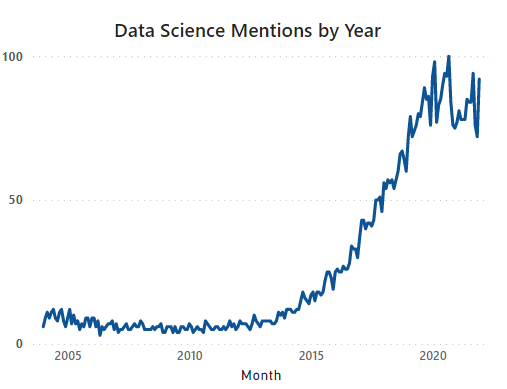
\includegraphics[width=0.5\textwidth]{figures/DataScience/trend_ds.png}
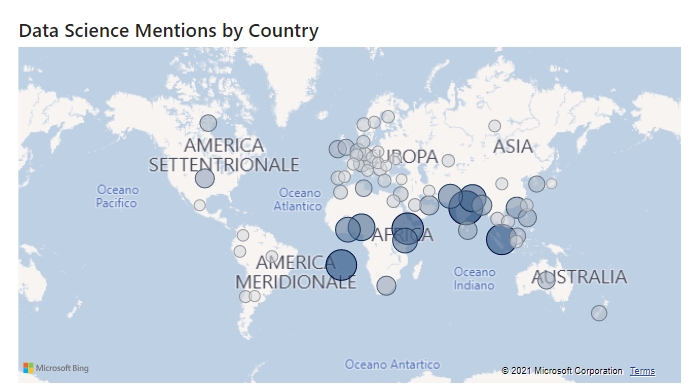
\includegraphics[width=0.5\textwidth]{figures/DataScience/map_ds.png}
}
\caption{
\textbf{Data Science Google searches}. Trends and geolocalization of Google searches of "data science" from 01/01/04 to 06/12/21.
} 
\label{fig:GoogleTrendsDS}
\end{figure}
That much so that it was awarded the title of \textquote{sexiest job of the 21st century} \cite{davenport2012sexiest}, and only American universities counted 78 data science programs in 2020 \cite{zhang2021data}.
However, the discussion over data science's essence has a long history, and multiple definitions have been proposed over the years \cite{donoho201750years}.
Although researchers and practitioners are yet to reach a complete agreement on its exact meaning  \cite{ASA2015statement}, \emph{five} common pillars can be identified by the various definitions.
First, \textbf{multidisciplinarity} is indisputably a key element stressed in every definition of data science. 
Second, as the name suggests, the \textbf{focus on data} and adequate techniques to manage and process them is inevitably an essential aspect.
Third, data science requires adopting suitable \textbf{analytical models} to transform data into knowledge.
Fourth, the \textbf{computing infrastructure} that is necessary to run data analysis timely and efficiently. 
Fifth, a compelling \textbf{visualization and communication} of the results that are simple enough to speak to a heterogeneous and non-technical audience, yet comprehensive of all relevant details to convey meaningful insights.

Inspired by these principles, this thesis describes the development of two data science projects and how the five pillars above are declined in practice.


\paragraph{Structure of the Thesis}

After an initial definition of the discipline of \emph{Data Science}, this thesis is organized as follows.

\Cref{chap:historyDS} draws a historical reconstruction of the evolution of the concept of data science over time, trying to clarify what this subject is all about and set an unambiguous reference framework. 

\Cref{partI} discuss in greater details the work presented in \citeA{morelli2021cresunet}. In particular, \Cref{chap:partI_intro} describes the technique of microscopic fluorescence and its application to life science and biology experiments. The task of counting objects in digital images is then presented, and some relevant available literature reviewed.
\Cref{chap:partI_dataset} describes the \textbf{Fluorescent Neuronal Cells} dataset \cite{clissa2021fluocells}, focusing on data acquisition, data annotations, and peculiar characteristics and challenges. 
In \Cref{chap:partI_methods}, the \textbf{cell ResUnet (c-ResUnet)} \cite{morelli2021cresunet} model is introduced and compared with some alternative architectures. Also, three experimental settings are detailed, which are then used for testing competing architectures through ablation studies.
In \Cref{chap:partI_results}, the performances achieved by the proposed approaches are evaluated both quantitatively and qualitatively.
Finally, \Cref{chap:partI_conclusions} summarizes the main findings of the study and discuss possible extensions.

\note[Luca][notesyellow]{TO BE COMPLETED WITH WHOLE STRUCTURE.}

\section{History of Data Science}
\label{chap:historyDS}

The first trace of this debate dates back to \cite{tukey1962future}, where Tukey uses the term \emph{data analysis} to indicate a discipline with the connotations of a \emph{science} and which is \textquote{defined by a ubiquitous problem rather than by a concrete subject}. 
Tukey's description incorporates many aspects seemingly tied closely to applied statistics: 
\begin{displayquote}
procedures for analyzing data, techniques for interpreting the results of such procedures, ways of planning the gathering of data to make its analysis easier, more precise or more accurate, and all the machinery and results of (mathematical) statistics which apply to analyzing data;
\end{displayquote}
Nevertheless, the extent Tukey attributes to data analysis is broader than its philological meaning, as it comprises all of statistics and embeds it in a larger entity \cite{huber2012data, donoho201750years}.
Indeed, Tukey himself sets the boundaries between data analysis and statistics in their respective binding to the strict formalism of mathematics.

In fact, he appeals for a looser attachment to mathematical foundations and suggests focusing on actionable insights rather than theory.
 - scope and usefulness over security
 - inadequate evidence shall suggest right answers
 - maths as judgment rather than proof
 
Finally, Tukey identified four driving forces in the emerging data analysis science:
Four major influences act on data analysis today:
1. The formal theories of statistics
2. Accelerating developments in computers and display devices
3. The challenge, in many fields, of more and ever larger bodies of data
4. The emphasis on quantification in an ever wider variety of disciplines

Despite being released 60 years ago, Tukey's description is incredibly modern and well depicts many activities currently under the umbrella of what we refer to as data science today.
Nonetheless, researchers and practitioners are yet to reach a complete agreement on its definition.

By and large, bla bla bla...

%----------------------------------------------------------------------------------------


% \part{First Part}
\label{partI}

\chapter{Introduction}
\label{chap:partI_intro}

Deep Learning models, and in particular Convolutional Neural Networks (CNNs) \cite{jimenez, greenspan}, have shown the ability to outperform the state-of-the-art in many computer vision applications in the past decade. 
Successful examples range from classification and detection of basically any kind of objects \cite{AlexNet, YOLO} to generative models for image reconstruction \cite{reconstruction} and super-resolution \cite{super-resolution}.
Thus, researchers from both academy and industry have started to explore adopting these techniques in fields such as medical imaging and bioinformatics, where the potential impact is vast.
For instance, CNNs have been employed for identification and localization of tumours \cite{brain_tumor,breast_cancer, ciresan2012deep, cirecsan2013mitosis}, as well as detection of other structures like lung nodules \cite{lung_nodules, meraj2020lung, su2021lung}, skin and breast cancer, diabetic foot \cite{TL_medical_imaging}, colon-rectal polyps \cite{korbar} and more, showing great potential in detecting and classifying biological features \cite{lundervold, sahiner, yadav}.

In the wake of this line of applied research, \Cref{partI} tackles the problem of counting cells into fluorescent microscopy pictures.

\section{Fluorescence microscopy 
% and life science experiments
}
\label{sec:fluorescence_microscopy}

\emph{Fluorescence} is a luminescence phenomenon that was first discovered in 1852 by George G. Stokes \cite{stokes2010memoir}. 
He observed that some molecules, denominated fluorophores, are susceptible to emitting light when they are in electronically excited states. These states can be caused by a physical mechanism (e.g. absorption of light), a mechanical process (e.g. friction) or chemical interactions.
% The widefield reflected light fluorescence microscope has been a fundamental tool for the examination of fluorescently labeled cells and tissues since the introduction of the dichromatic mirror in the late 1940s. Furthermore, advances in synthetic fluorophore design coupled to the vast array of commercially available primary and secondary antibodies have provided the biologist with a powerful arsenal in which to probe the minute structural details of living organisms with this technique. In the late twentieth century, the discovery and directed mutagenesis of fluorescent proteins added to the cadre of tools and created an avenue for scientists to probe the dynamics of living cells in culture.
In other words, fluorescence is the property of some atoms and molecules to absorb light at a specific wavelength. In turn, this causes a transition from a ground state to an excited one. When that happens, the fluorophore becomes unstable and releases the absorbed energy by emitting light of a longer wavelength (Stokes shift) to get back to the ground state.
This difference in wavelengths between the absorbed and emitted light is the enabling factor of microscopic fluorescence. 
In practice, synthetic fluorophores having desired fluorescence properties are adopted, and the 
instrumentation is carefully set up to illuminate the specimen with a precise wavelength. The Stokes shift is then exploited to filter out the exciting light without blocking the emitted fluorescence, thus making the fluorescent objects visible \cite{lichtman2005fluorescence}.

Many experiments in the life science domain are based on this technique.
Specifically, the fluorophore is designed to couple with the molecular structures of interest and interact with the tissues under study. 
% In this way, the activity/presence of the targeted compounds is tracked in different experimental conditions (e.g. different treatments). their efficacy is assessed  by counting ...
In this way, the efficacy of a treatment or the organism response to a given environment is assessed by tracking the activity/presence of the targeted compounds. 
This process often resorts to counting how many molecular structures produced fluorescent emissions in the different conditions \cite{hitrec2019neural, hitrec2021reversible, da2020median}.
For example, \citeA{hitrec2019neural} investigated the brain areas of mice that mediate the entrance into torpor, showing evidence of which networks of neurons are associated with this process.

Torpor, also referred to as dormancy, is a behavioral and physiological state often observed in both animals and plants. 
In particular for animals, this condition is typically characterized by reduced body temperature and depressed metabolism, and it is exploited by living organisms in response to a variety of hostile environmental stimuli, including low temperature and water or food deprivation \cite{GANSLOER2019328, WITHERS2019309}.
Interestingly, some studies have shown how this condition can be artificially induced thanks to radiations, which could be crucial for a broad spectrum of medical purposes.
Certainly,
knowing the mechanisms that rule the onset of lethargy, and understanding how to trigger their activation,  may have a significant impact when coming to human applications.
% Indeed, artificially inducing hibernation may be crucial for a broad spectrum of medical purposes.
For instance, such an approach could be very beneficial when dealing with patients who need invasive surgery, e.g. intensive care or oncology treatments \cite{bouma2012induction, alam2012hypothermia, bellamy1996suspended}.
Pushing the imagination even further, one could think of hibernation as an enabling factor for long interplanetary trips, where astronauts could overcome or limit side effects of space travels \cite{CERRI20161, CERRI2021218, bradford2020aerospace}.

As a result of all these implications, it becomes evident how the matter assumes considerable interest and qualifies for further in-depth studies.
Nevertheless, the technical complexity and the manual burden of these analyses often hampers fast developments in the field.
Indeed, these experiments typically rely heavily on semi-automatic techniques that involve multiple steps to acquire and process images correctly.  
Manual operations like area selection, white balance, calibration and color correction are fundamental in order to identify neurons of interest successfully \cite{luppi1, luppi2, luppi3}. 
As a consequence, this process may be very time-consuming depending on the number of available images. 
Also, the task becomes tedious when the objects appear in large quantities, thus leading to errors due to fatigue of the operators.
Finally, a further challenge is that sometimes structures of interest and picture background may look similar, making them hardly distinguishable. When that is the case, counts become arguable and subjective due to the interpretation of such borderline cases, thus leading to an intrinsic arbitrariness.

For these reasons, this work aims at facilitating and speeding up future research in this and similar fields through the adoption of a CNN that counts the objects of interest without human intervention.
% Therefore, the introduction of automatic procedures to detect and count objects in digital images would bring four main benefits in such applications:
% \begin{itemize}
%     \item speeding up the operations,
%     \item lightening the efforts of researchers
%     \item limiting fatigue errors,
%     \item standardizing to the systematic effect of the model the arbitrariness due to multiple operators influence.
% \end{itemize}
The advantages of doing so are two-fold. 
On one side, the benefit in terms of time and human effort saved through the automation of the task is evident.
On the other, using a Deep Learning model would impede fatigue errors and introduce a systematic ``operator effect".
In this way, the annotation would result in a more coherent process and it would guarantee similar structures are labeled consistently, both within the same experiment and across research groups.
% thus limiting the arbitrariness of borderline cases both within and between experiments.


\section{Counting objects in images}
\label{sec:counting_objs}

Counting objects in digital images is a common task for many real-world applications \cite{segui2015learning, arteta2016counting, paul2017countception, rahnemoonfar2017deepfruit} and different approaches have been explored to automate it \cite{lempitsky2010learning, ciresan2012deep, cirecsan2013mitosis, Kraus2016, Raza2017}. 

Multiple paradigms for counting objects in images have been proposed depending on the study's specific needs and the available data.
The natural setting to tackle this problem is the so-called \textit{counting-by-regression} scheme. 
In this case, the input data consist of the image and, optionally, other features. 
The model is then trained to output the raw count of objects directly. However, this approach does not provide any immediate justification of which elements generated the final count.
Another strategy is \textit{counting-by-detection}.
In this case, the model is trained to reproduce ground-truth masks having bounding boxes surrounding the objects to detect. 
In this way, the output becomes an image where pixels are classified either into the signal class (within the boxes) or as background (outside). 
This outcome provides the raw count as the number of sets of connected pixels, plus a justification in terms of the localization furnished by the bounding boxes. 
Building on the latter framework, one can refine the model's ability to detect and localize the objects by including semantic labels for each pixel in the ground-truth masks. This allows pixel-wise classification that enables to discern the exact boundaries of each object. The total count is then retrieved again by looking at groups of connected pixels. Such an approach is referred to as \textit{counting-by-segmentation}.
This work is framed under the latter paradigm so to support the results with a clear, visual evidence of which objects contribute to the final counts.

\subsection{Related works}
\label{sec:related_works}

Some interesting approaches have been proposed for detecting and counting cells in microscopic images.
\citeA{Faustino2009} propose an automated method leveraging the luminance information to generate a graph representation from which counts of cells are retrieved after a careful mining process. Nonetheless, their approach relies on the manual setting of some parameters, like the optimal threshold for separating cell clusters and the luminance histogram binning adopted for retrieving connected components, which hampers the extension to different data.

\citeA{unet} present a Deep Learning approach for segmentation of cells in an image. 
Their main contribution is the introduction of a novel network architecture, \textit{U-Net}, which is still state-of-the-art in several applications with only slight adaptations \cite{masin2021novel, ritch2020axonet}. 
The basic idea is to have an initial contracting branch used to capture relevant features, and a symmetric expanding one that allows for accurate localization.
The main drawback is that its enormous number of parameters requires relevant computing power and makes the training difficult because of vanishing gradient \cite{vanishing_gradient}. 
For this reason, a commonly used variation adopts residual units \cite{residual_units} with short-range skip-connections and batch normalization to prevent that problem.
Also, this typically guarantees comparable performance with much less parameters.

% Two further proposals are detailed in the 2016 Kraus et al. \cite{Kraus2016} paper and in the 2017 Raza et al. \cite{Raza2017} paper.
\citeA{Kraus2016} combine deep CNNs with multiple instance learning in order to classify and segment microscopy images using only whole image level annotations. 
\citeA{Raza2017} propose a novel multiple-input multiple-output convolution neural network (MIMO-Net) that utilizes multiple resolutions of the input image, connects the intermediate layers for better localization and context and generates the output using multi-resolution deconvolution filters.

A common downside of these approaches is  the need of ground-truth labels (or masks) with accurate annotations of whether each pixel belongs to an object (in this case a cell) or the background, resulting in an additional and laborious data preparation phase.
% Two further interesting approaches that have been considered are detailed in the 2016 Kraus et al. \cite{Kraus2016} paper and in the 2017 Raza et al. \cite{Raza2017} paper.
% The former suggested a method that combined deep CNNs with multiple instance learning (MIL) in order to classify and segment microscopy images using only whole image level annotations. The latter proposed a novel multiple-input multiple-output convolution neural network (MIMO-Net) that utilizes multiple resolutions of the input image, connects the intermediate layers for better localization and context and generates the output using multi-resolution deconvolution filters.
In an attempt to overcome this limitation, some works try to tackle the problem in an unsupervised fashion. For example, \citeA{Riccio2019} address segmentation and counting with a step-wise procedure. The whole image is first split into square patches, and a combination of gray level clustering followed by adaptive thresholding is adopted for foreground/background separation. Individual cells are then labeled by detecting their centers and applying a region growing process. 
While this procedure bypasses the need for ground-truth masks, it still requires handcrafted hyperparameters selection that needs to be tuned for new data.
For additional examples of segmentation in biological images, please refer to \citeA{Riccio2019}.

\section{Contribution}
\label{sec:contribution}
\sidenote[Luca][notesyellow]{Questa parte va rivista più avanti in base ai prossimi sviluppi}
% Drawing from existing literature, our work
The first part of this thesis tackle the issue of automating cell counting in fluorescence microscopy using Deep Learning. 
Building upon \citeA{morelli2021cresunet}, the following focuses on a supervised learning approach in the context of semantic segmentation.
% This choice is justified by the aim to provide a solution with a strong emphasis on interpretability, so to build trust in the end users and encourage its adoption by the scientific community. 
% In this respect, also justifying the output number through a segmentation map that localizes the detected objects.  
% This additional information is particularly relevant to corroborate the results with a clear, visual evidence of which cells contribute to the final counts.
The main contributions of this work are the following. 
First, the development of an automatic approach for counting neuronal cells. 
In particular, two families of network architectures are compared, the {Unet} and its variation \textit{ResUnet}, in terms of counting and segmentation performance. 
Second, ablation studies are conducted to show how using weight maps that penalize errors on cell boundaries promotes accurate segmentation, especially in cluttered areas.
Last but not least, the pre-trained model%
\footnote{\linkmodel}
and a rich dataset with the corresponding ground-truth annotations \cite{clissa2021fluocells} are released to foster methodological research in both biological imaging and deep learning communities.
\chapter{Fluorescent neuronal cells dataset}
\label{chap:partI_dataset}

\begin{figure}%[!b]
\begin{subfigure}{1.1\textwidth}
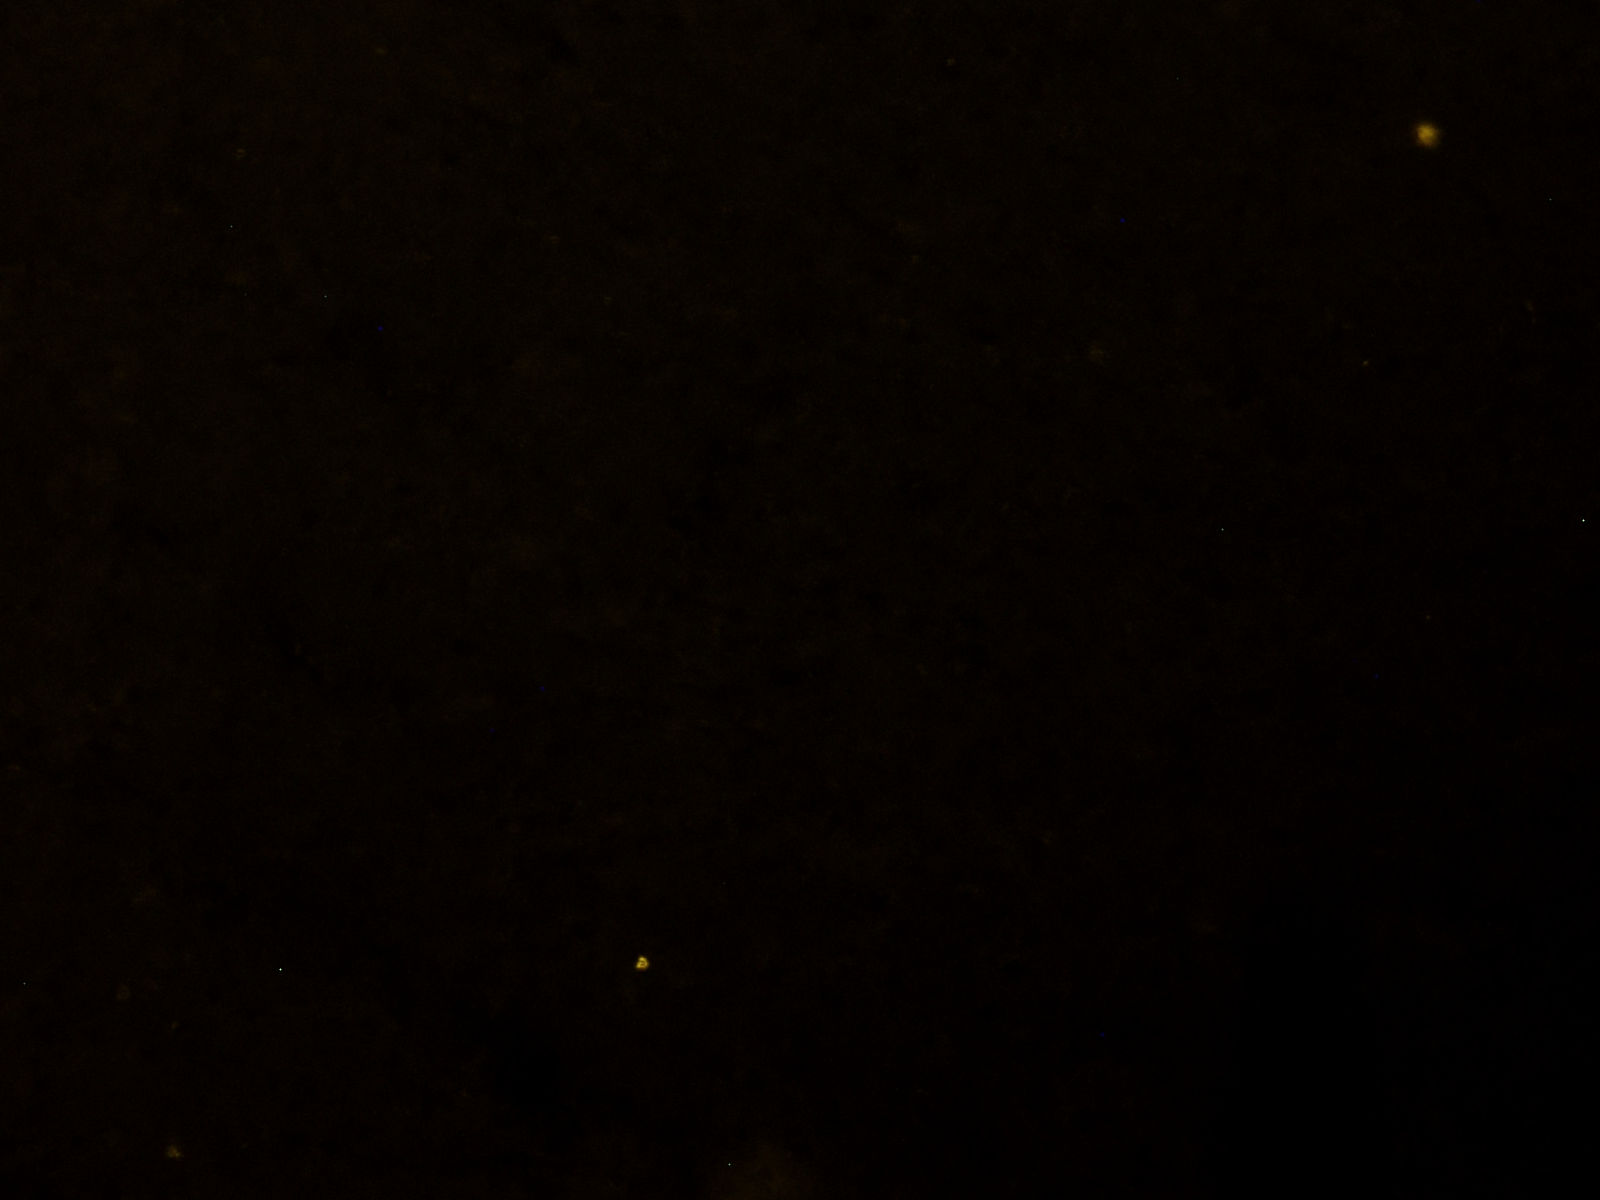
\includegraphics[width=0.5\linewidth]{figures/120_dataset/i_empty.png}
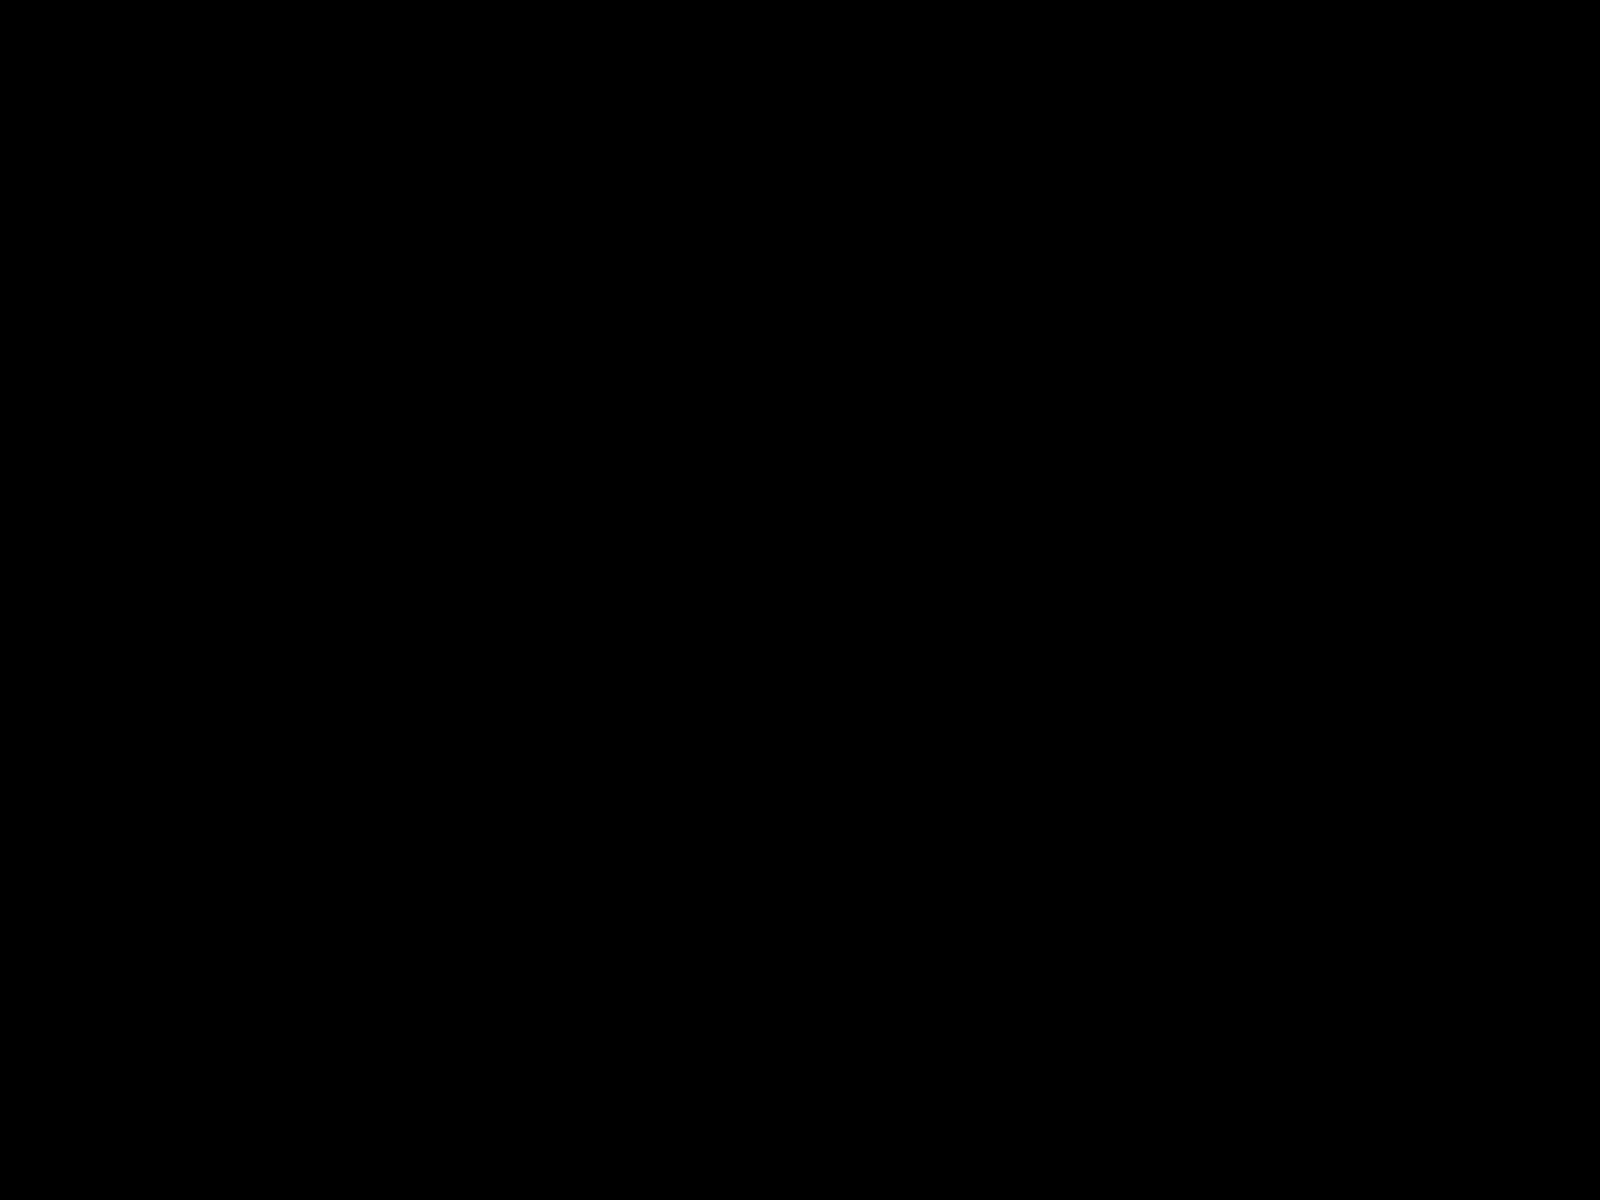
\includegraphics[width=0.5\linewidth]{figures/120_dataset/m_empty.png}
\subcaption{}
\label{fig:dataset:empty}
\end{subfigure}

\centering
\begin{subfigure}{1.1\textwidth}
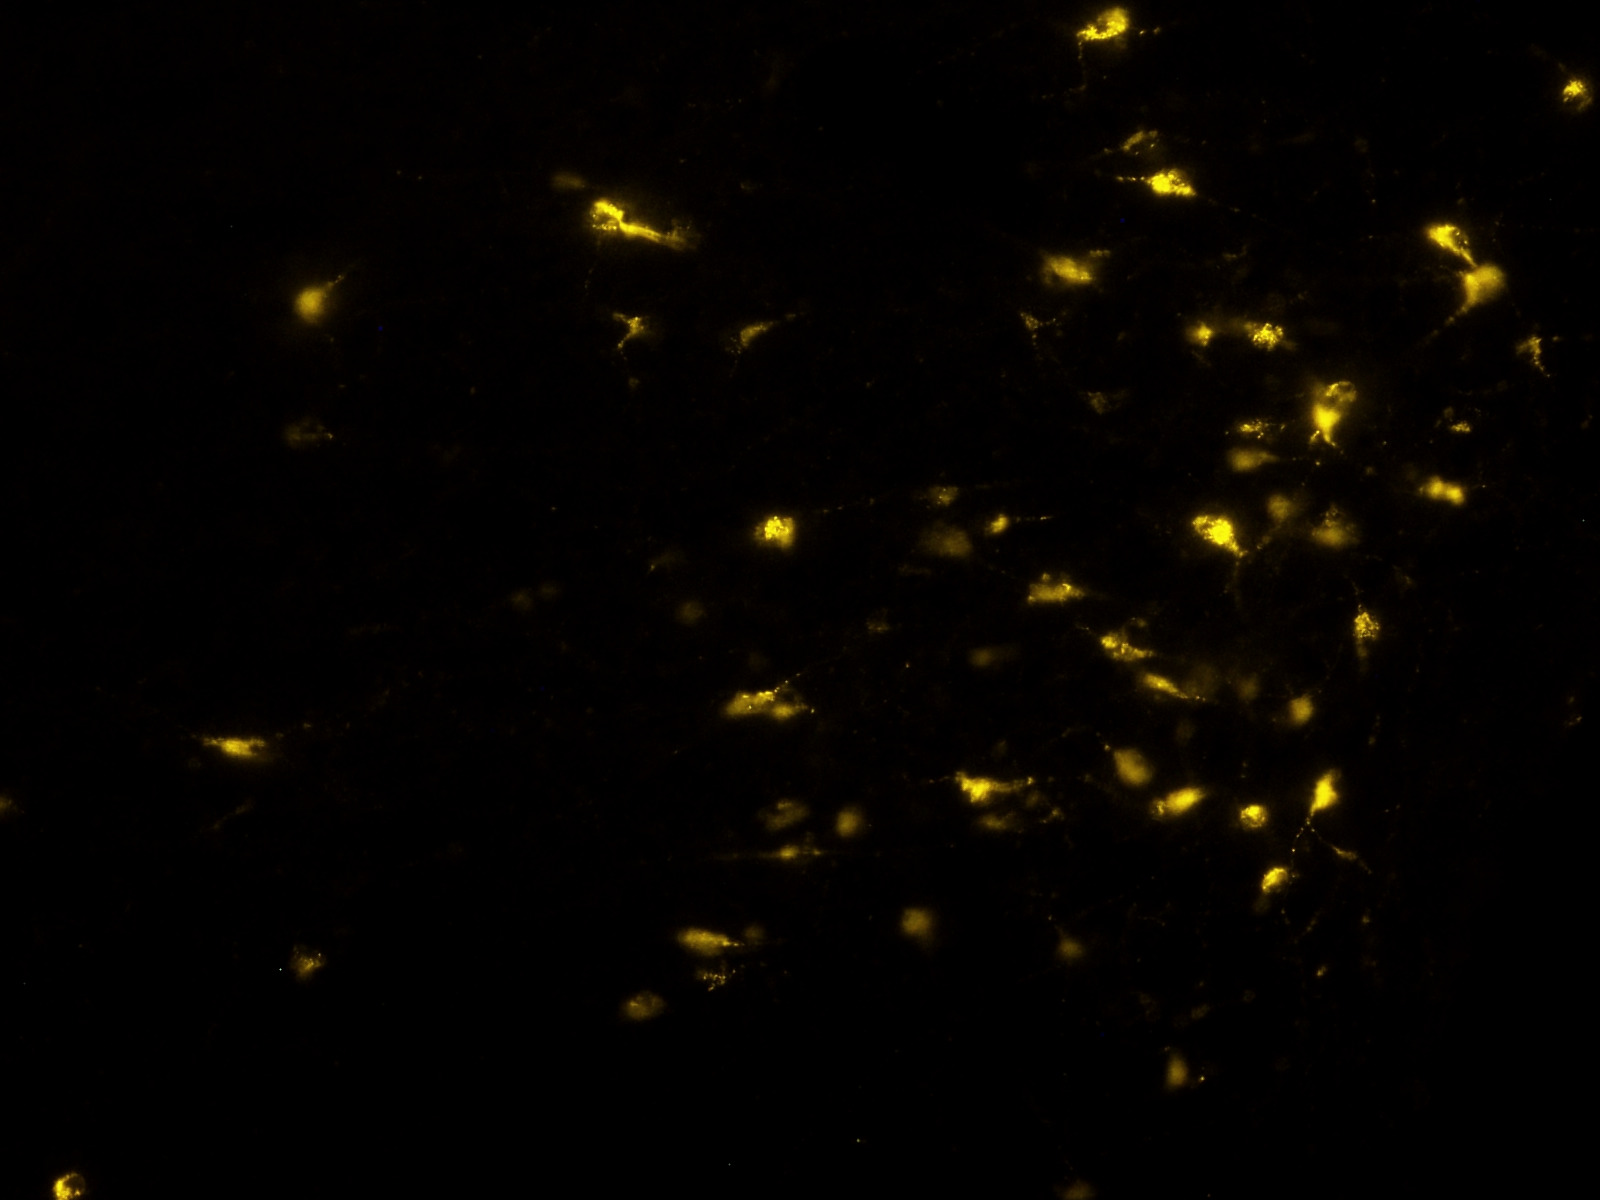
\includegraphics[width=0.5\linewidth]{figures/120_dataset/i_168.jpeg}
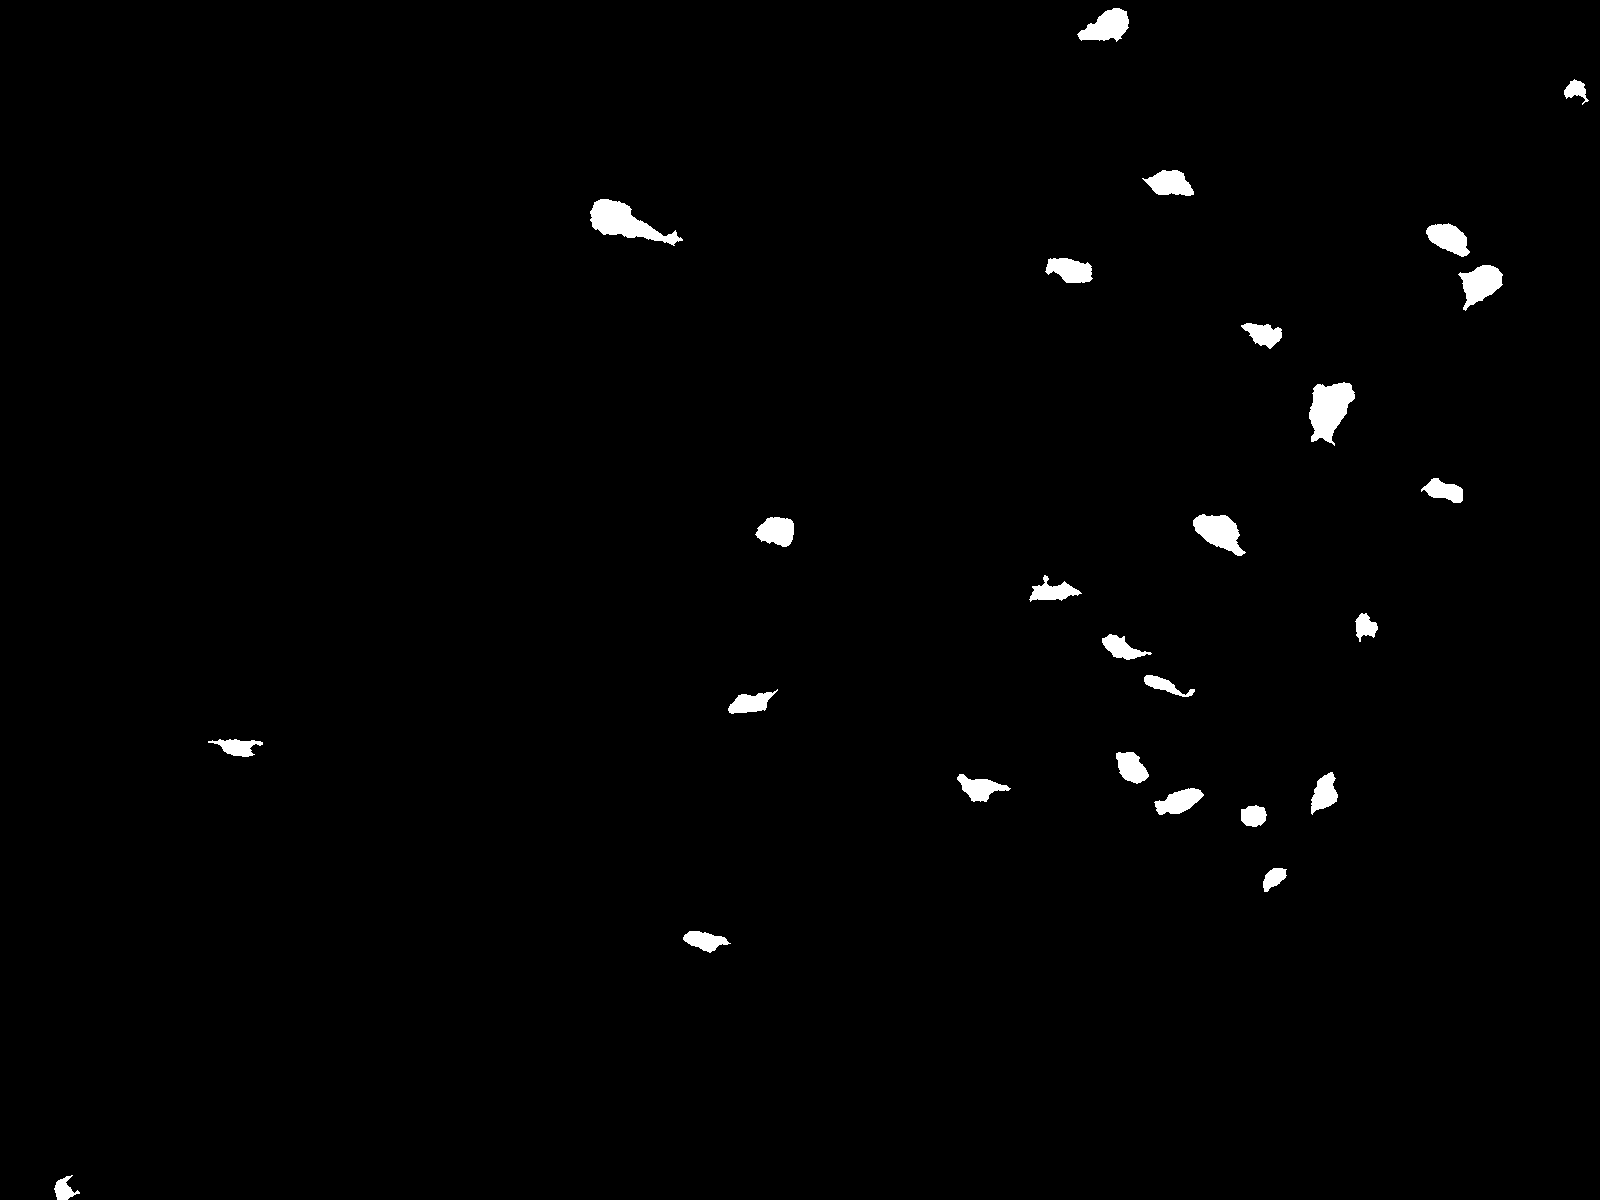
\includegraphics[width=0.5\linewidth]{figures/120_dataset/m_168.png}
\subcaption{}
\label{fig:dataset:dark}
\end{subfigure}

\centering
\begin{subfigure}{1.1\textwidth}
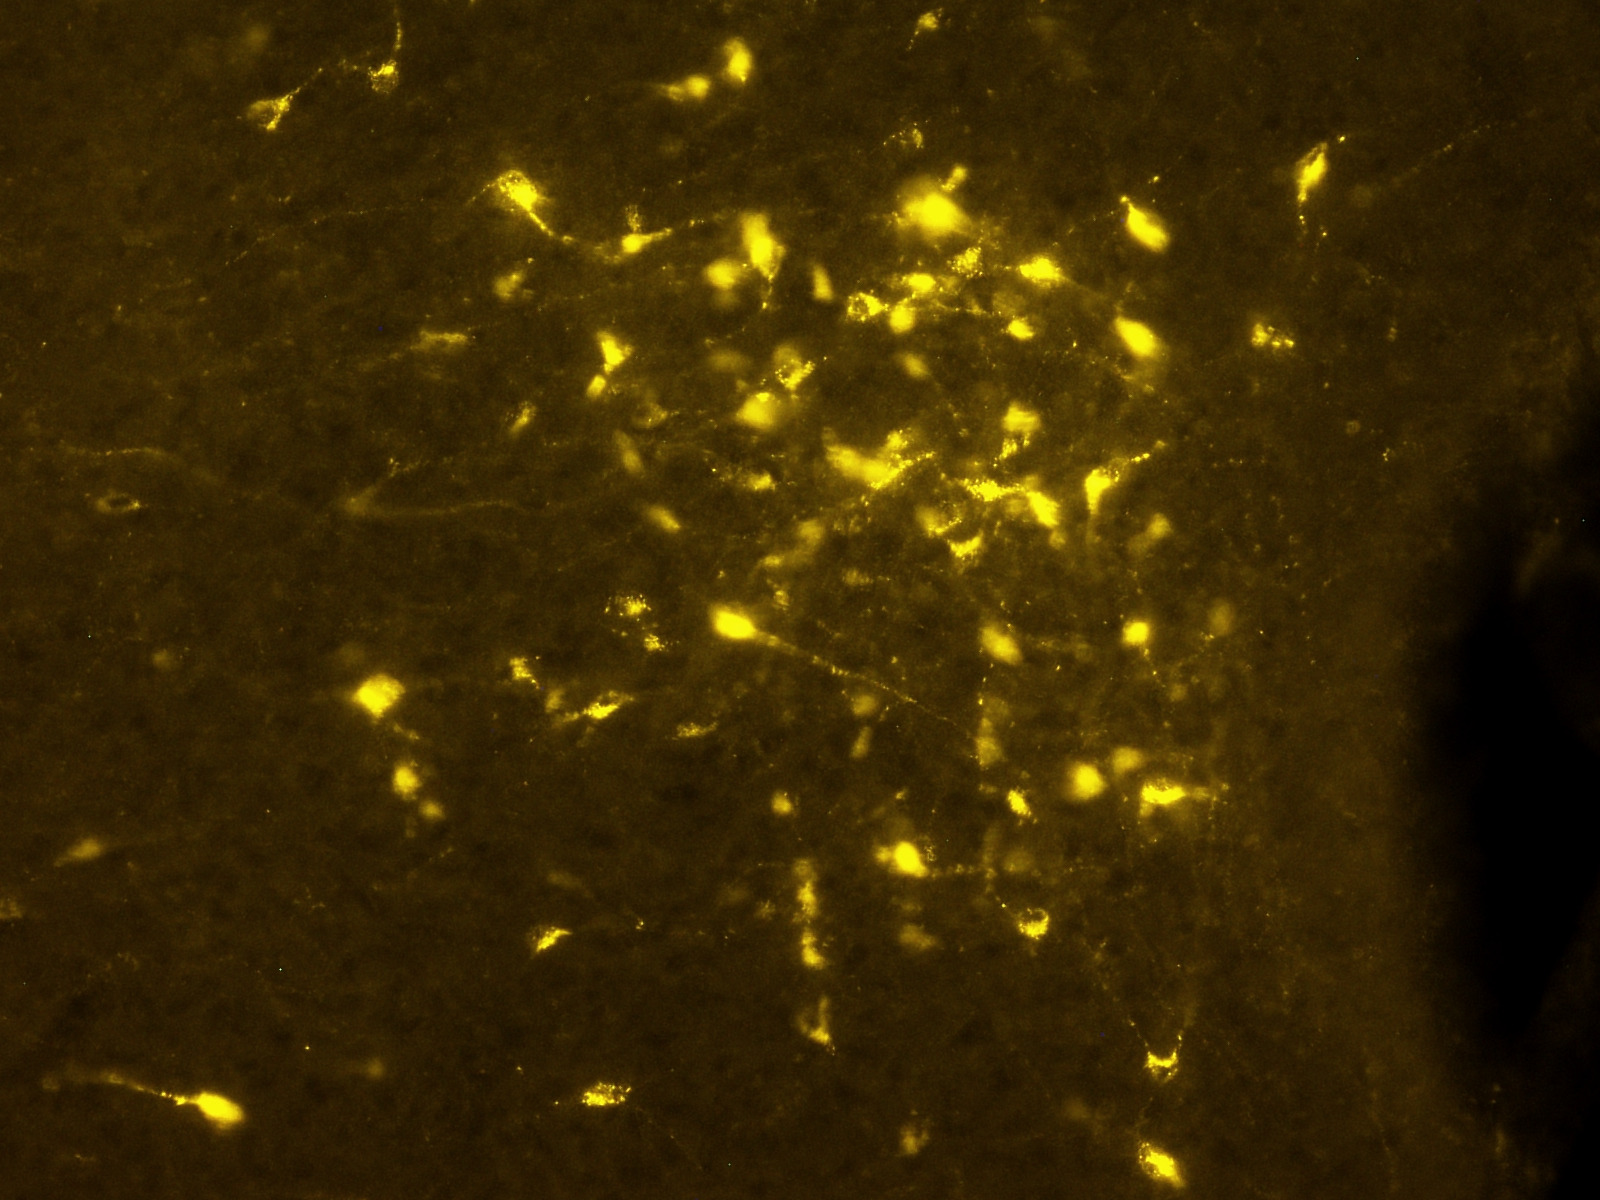
\includegraphics[width=0.5\linewidth]{figures/120_dataset/i_257.jpeg}
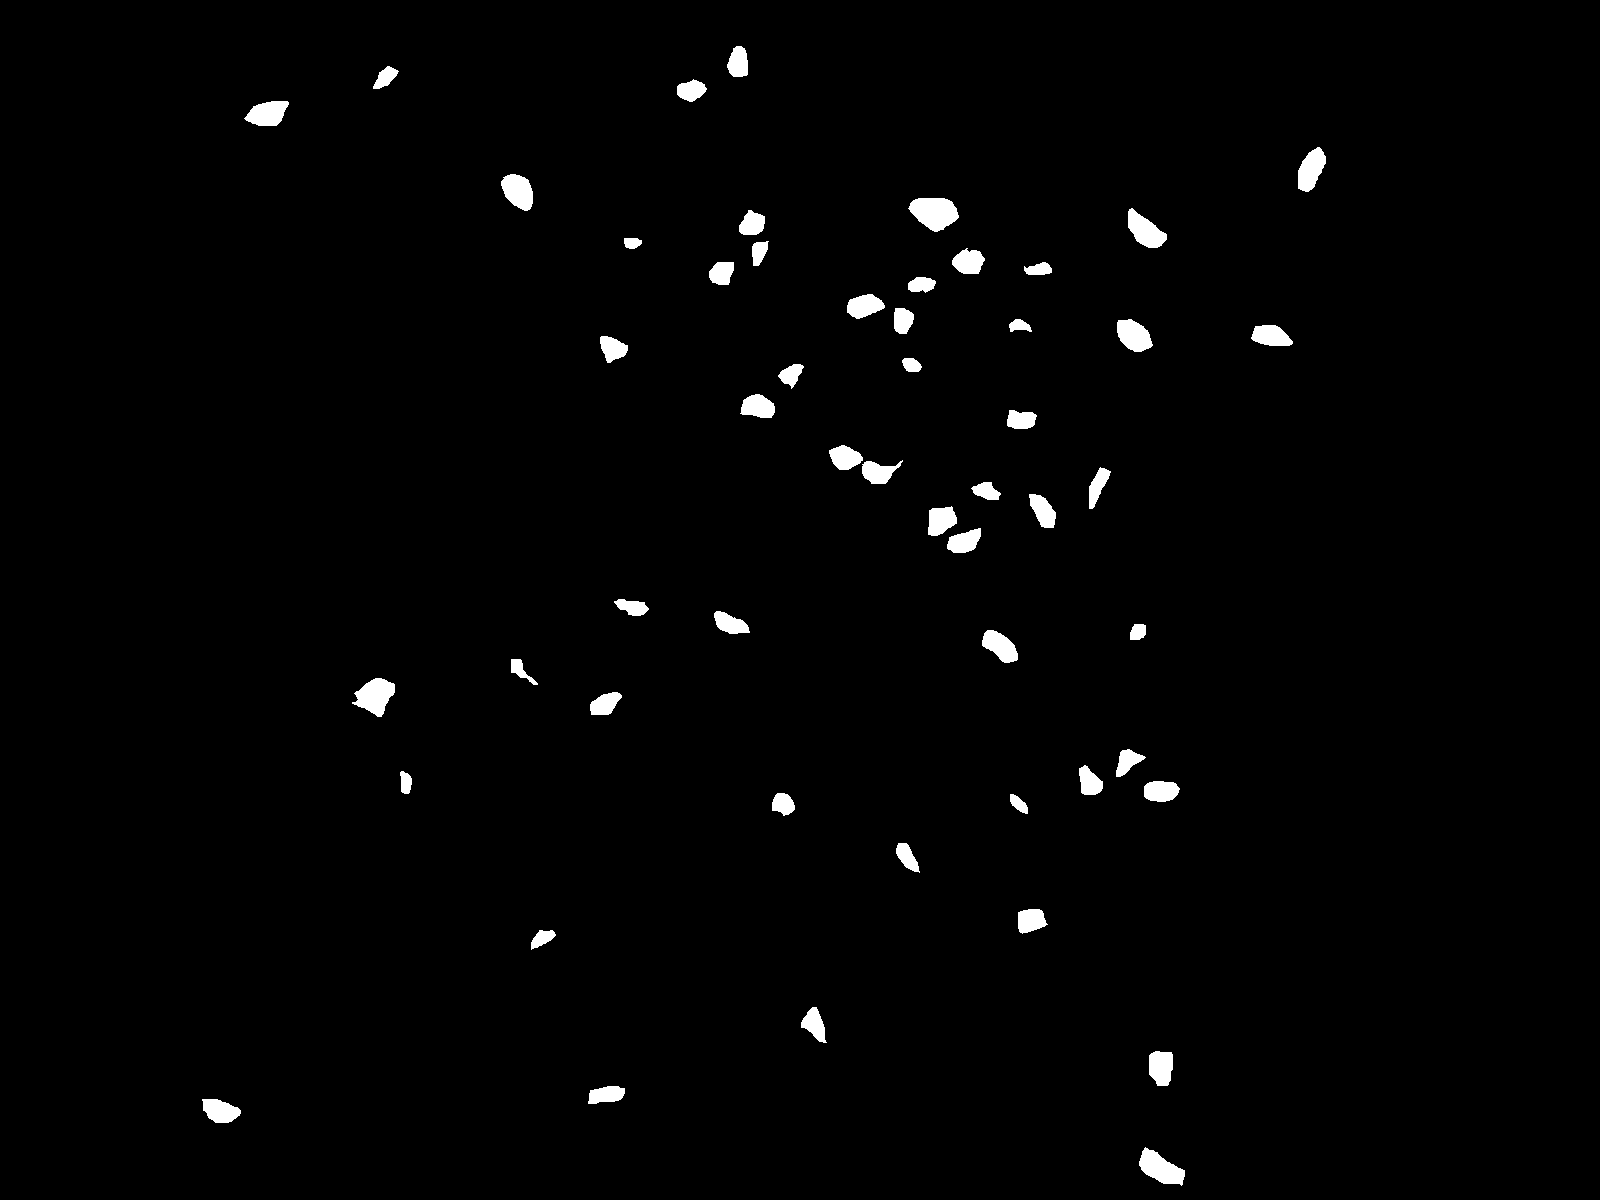
\includegraphics[width=0.5\linewidth]{figures/120_dataset/m_257.png}
\subcaption{}
\label{fig:dataset:bright}
\end{subfigure}
\vspace{-0.2cm}
\caption{
\textbf{Sample data}. 
Original images (left) and corresponding ground-truth masks used for training (right).
% The original images (left) present neuronal cells of different shape, size and saturation over a background of variable brightness and color.
% The corresponding ground-truth masks used for training (right) depicts cells as white pixels over a black background.
} \label{fig:dataset}
\end{figure}%
\begin{figure}%[ht]\ContinuedFloat
\centering
\begin{subfigure}{1.1\textwidth}
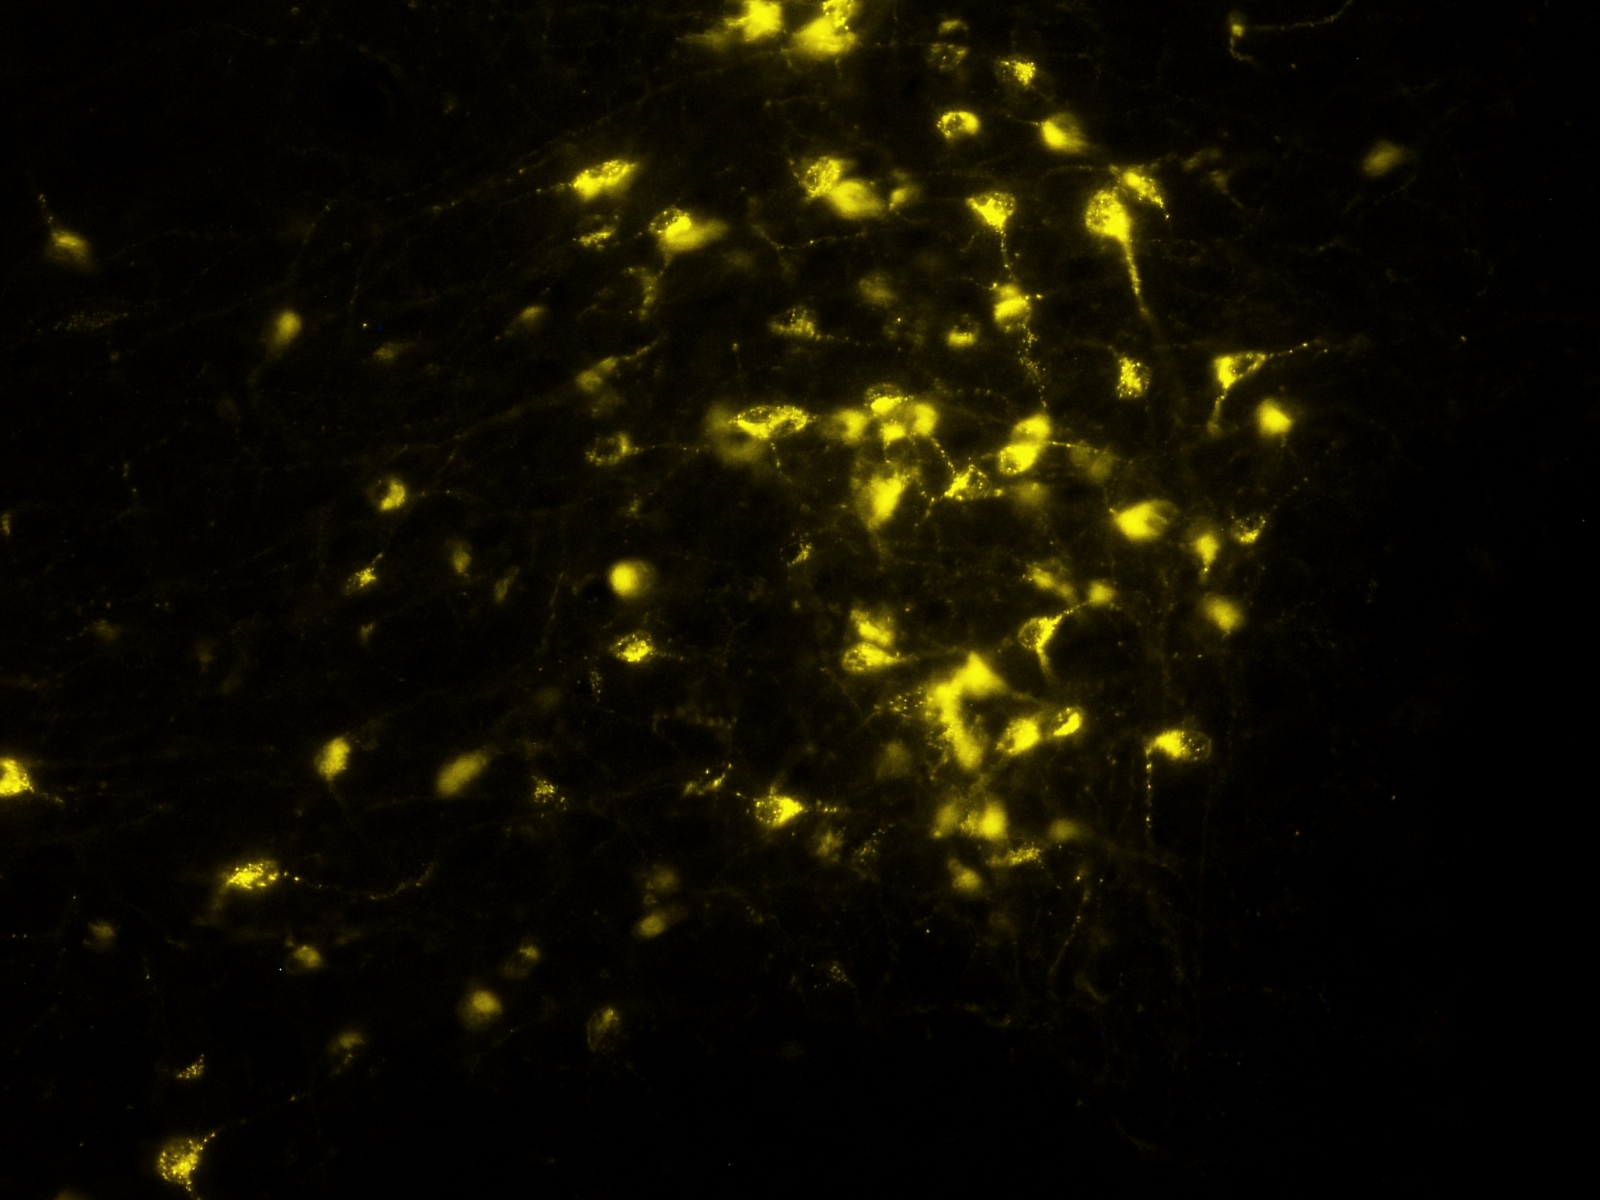
\includegraphics[width=0.5\linewidth]{figures/120_dataset/i_clumping_yellow.png}
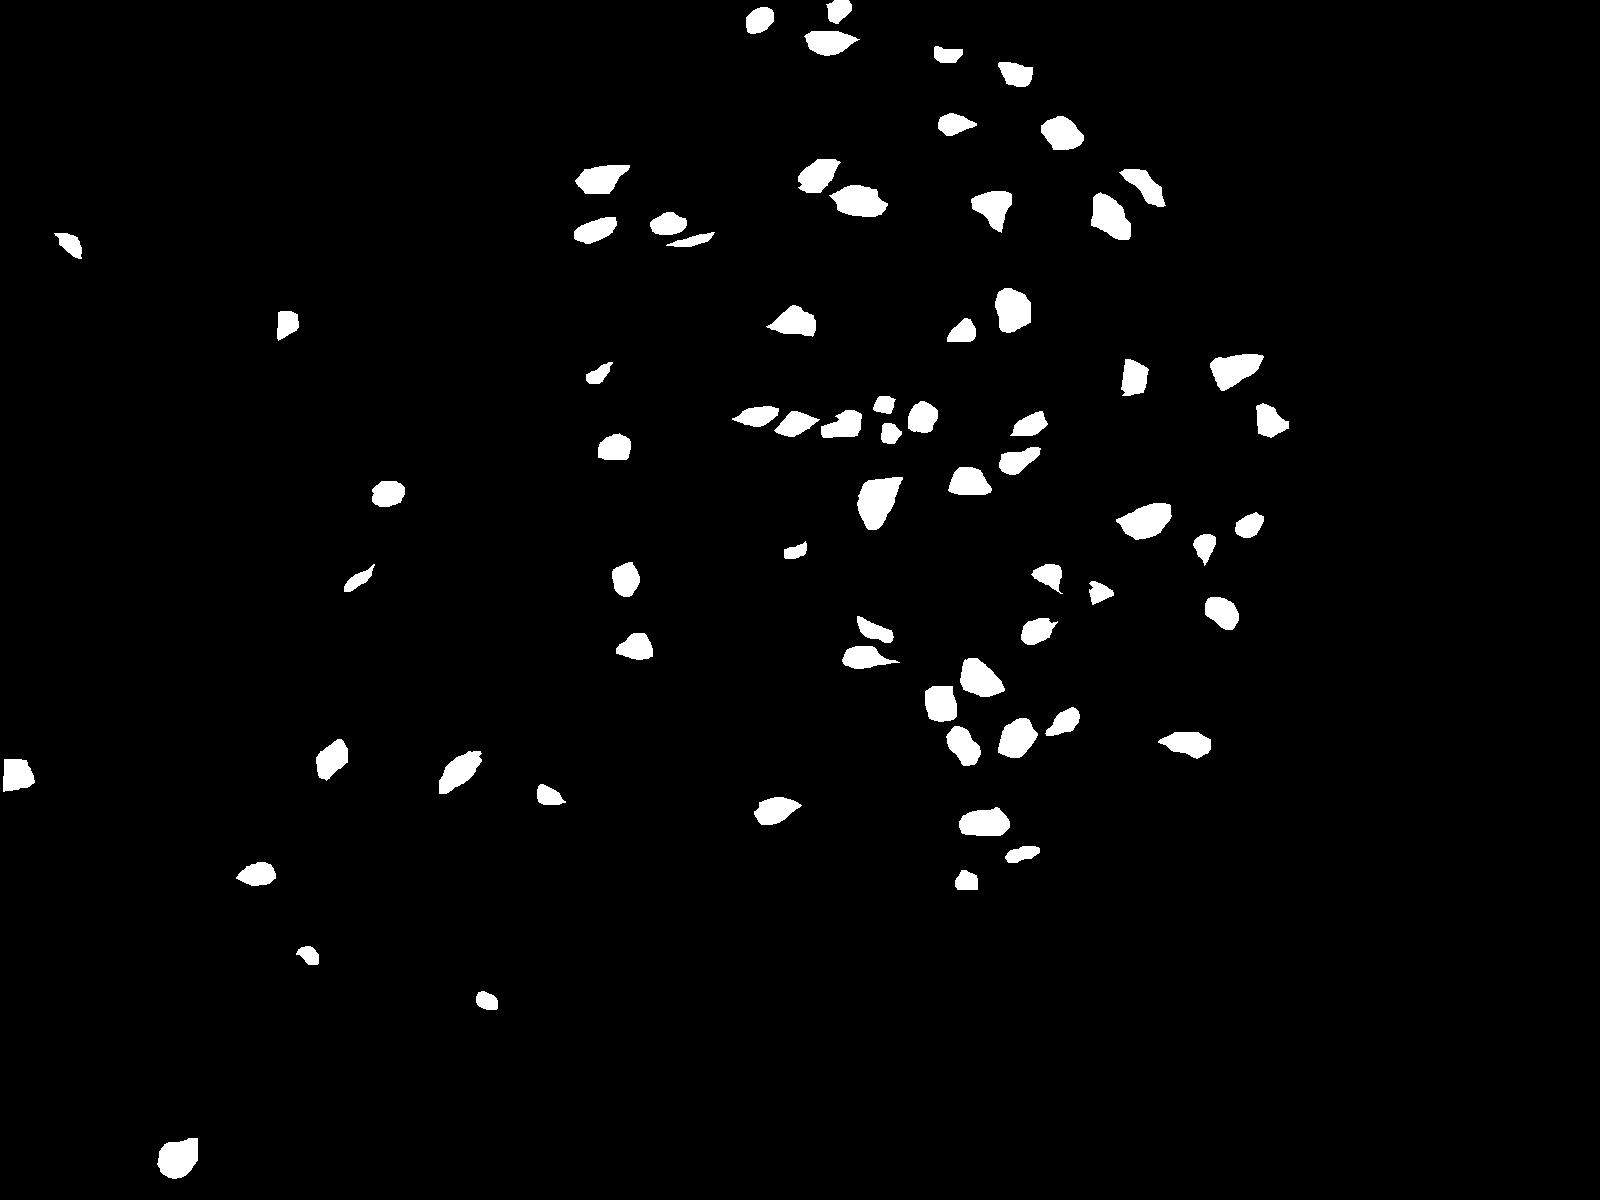
\includegraphics[width=0.5\linewidth]{figures/120_dataset/m_clumping_yellow.png}
\subcaption{}
\label{fig:artifacts:clumping}
\end{subfigure}

\centering
\begin{subfigure}{1.1\textwidth}
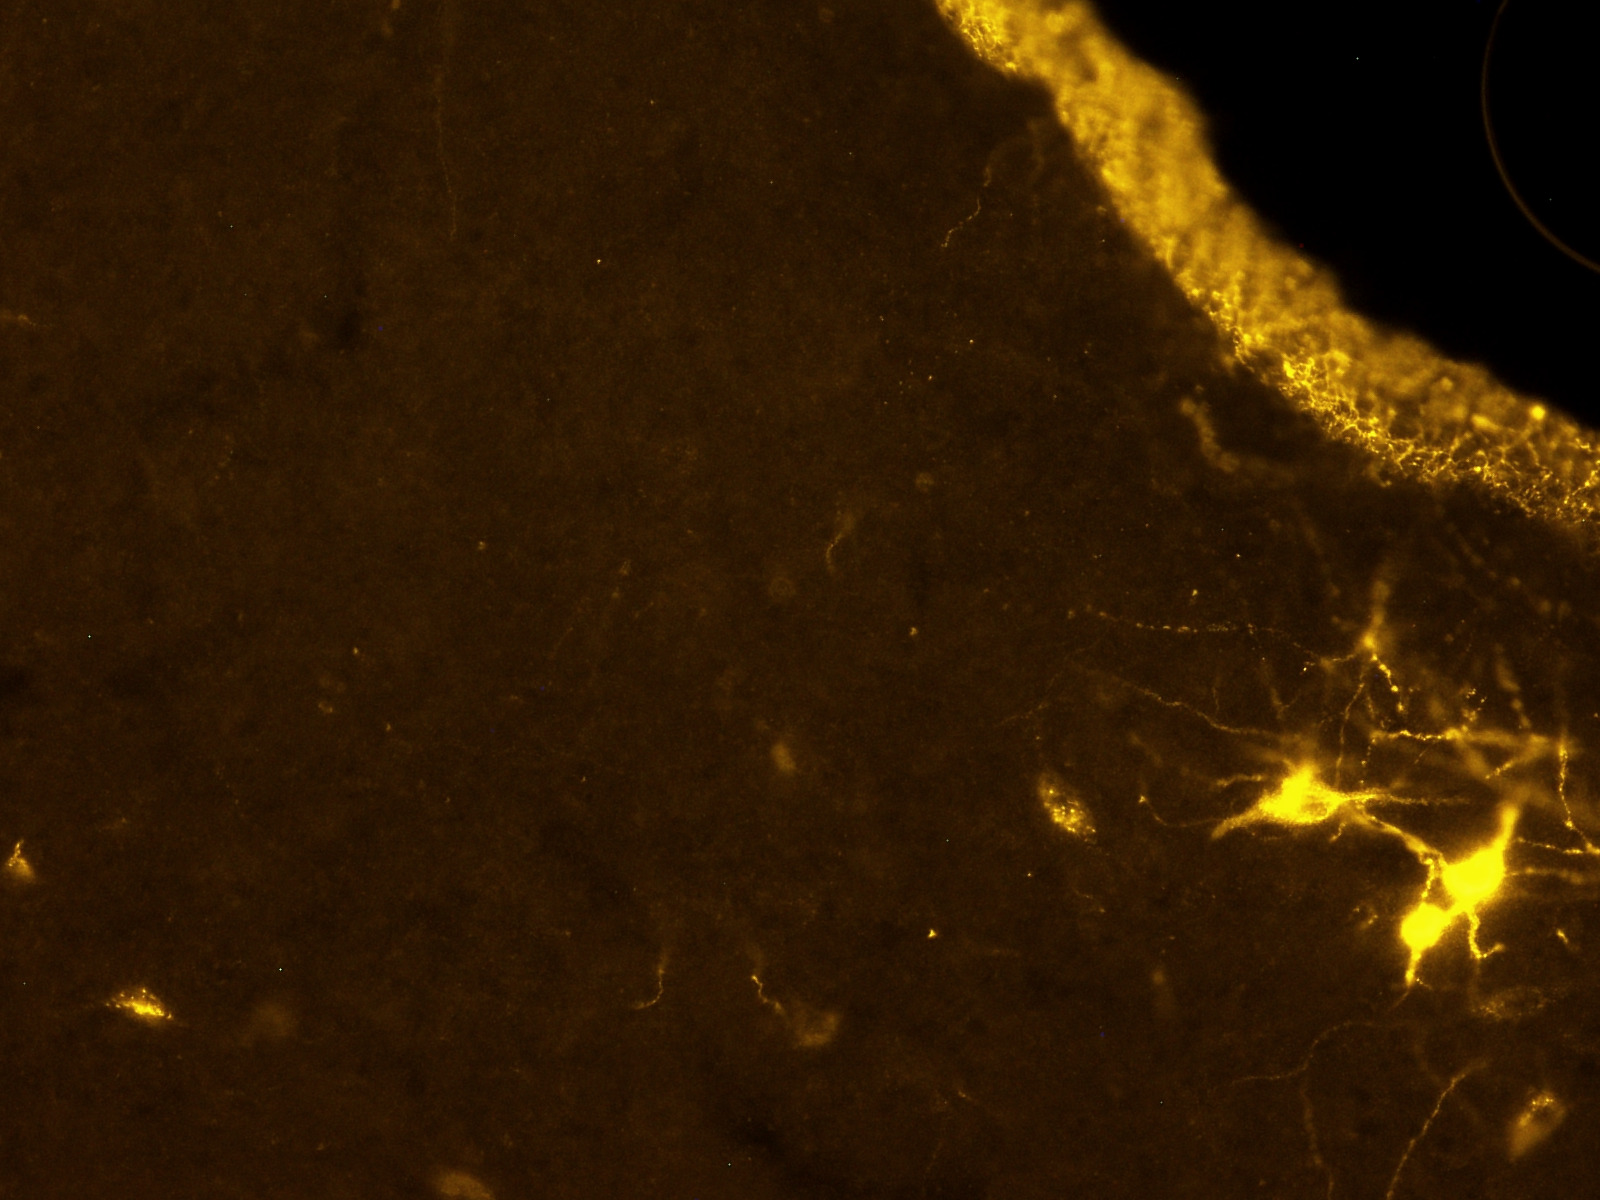
\includegraphics[width=0.5\linewidth]{figures/120_dataset/i_252.jpeg}
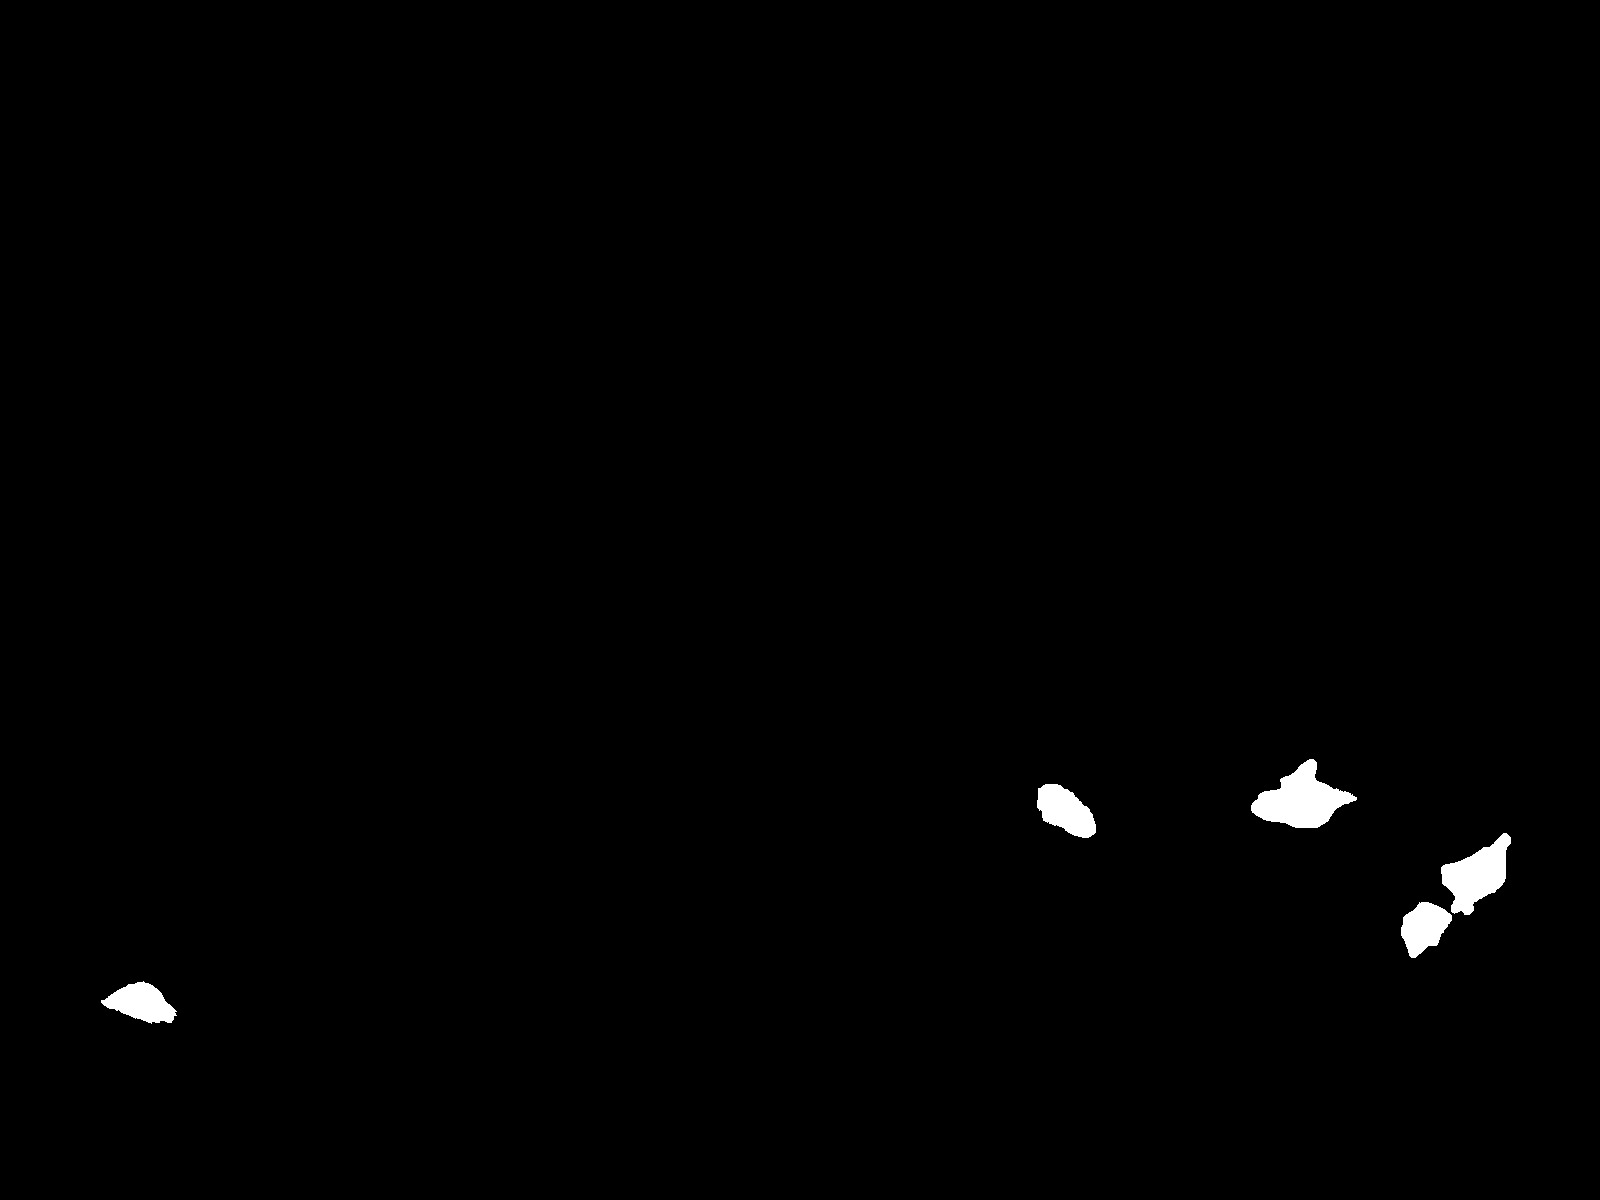
\includegraphics[width=0.5\linewidth]{figures/120_dataset/m_252.jpeg}
\subcaption{}
\label{fig:artifacts:stripe}
\end{subfigure}
\centering
\begin{subfigure}{1.1\textwidth}
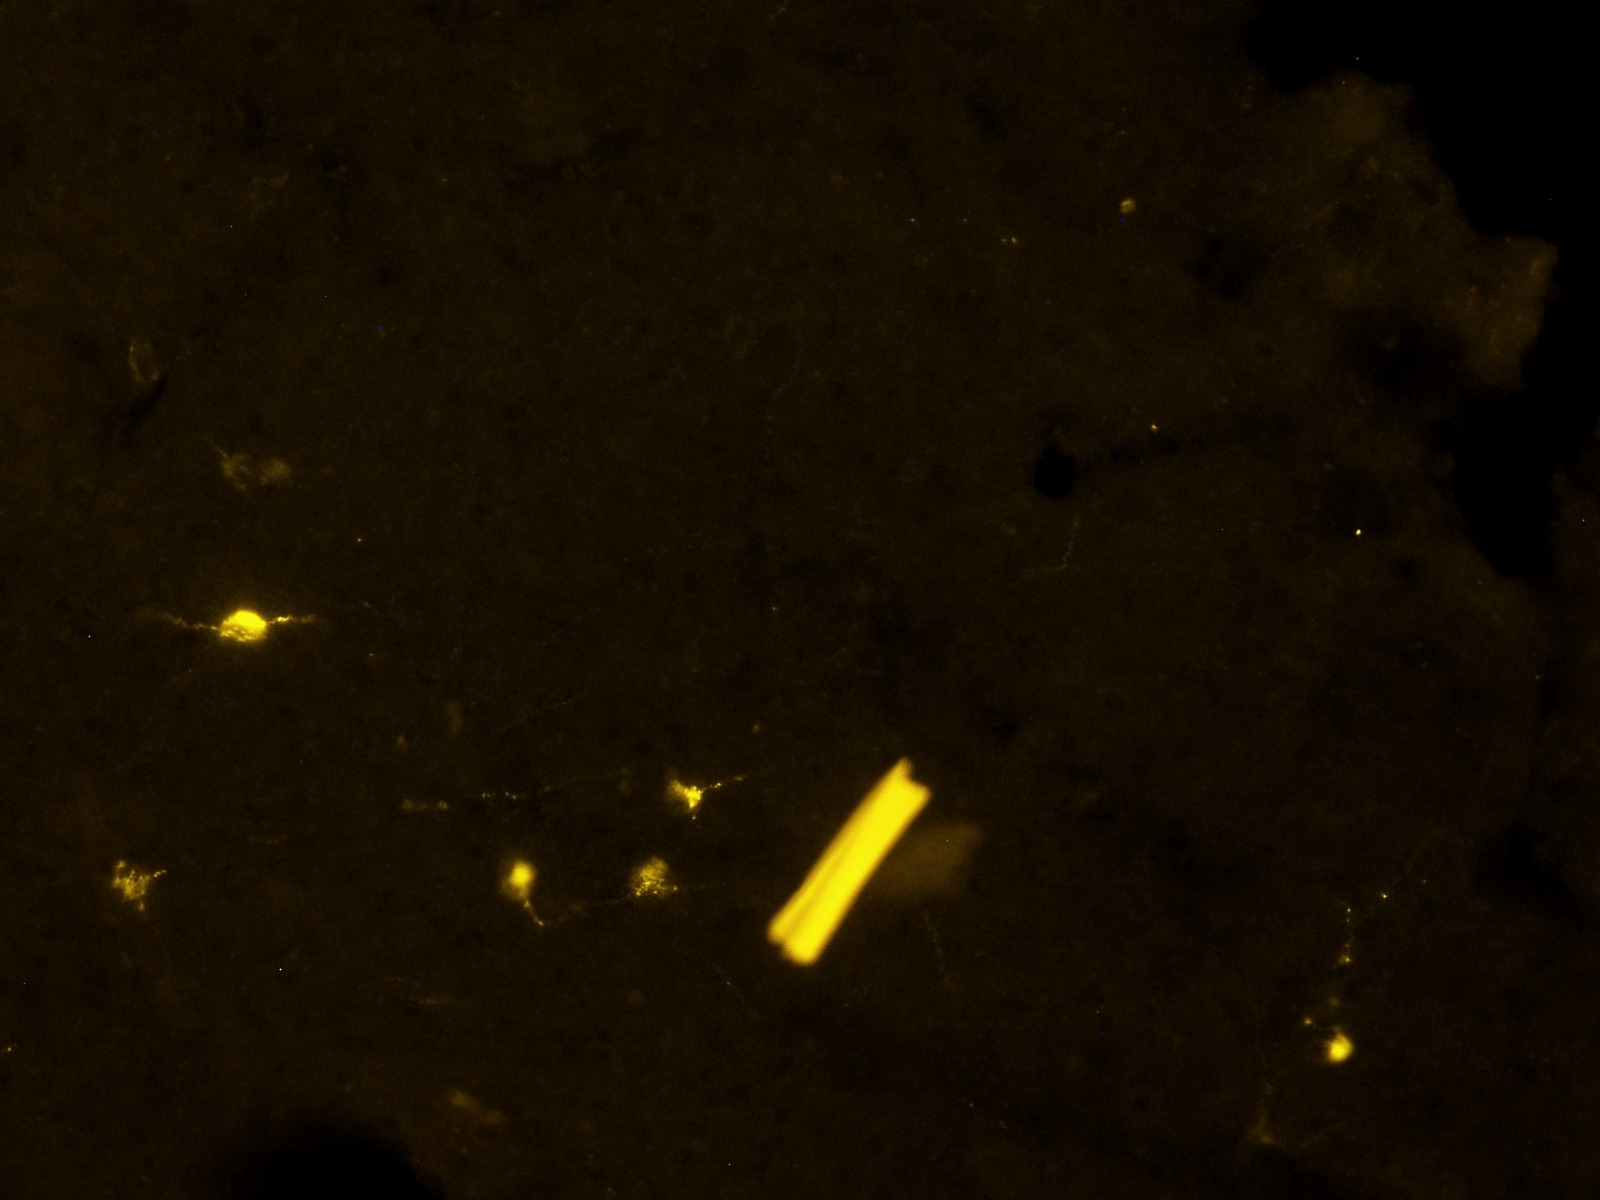
\includegraphics[width=0.5\linewidth]{figures/120_dataset/i_maccherone.jpeg}
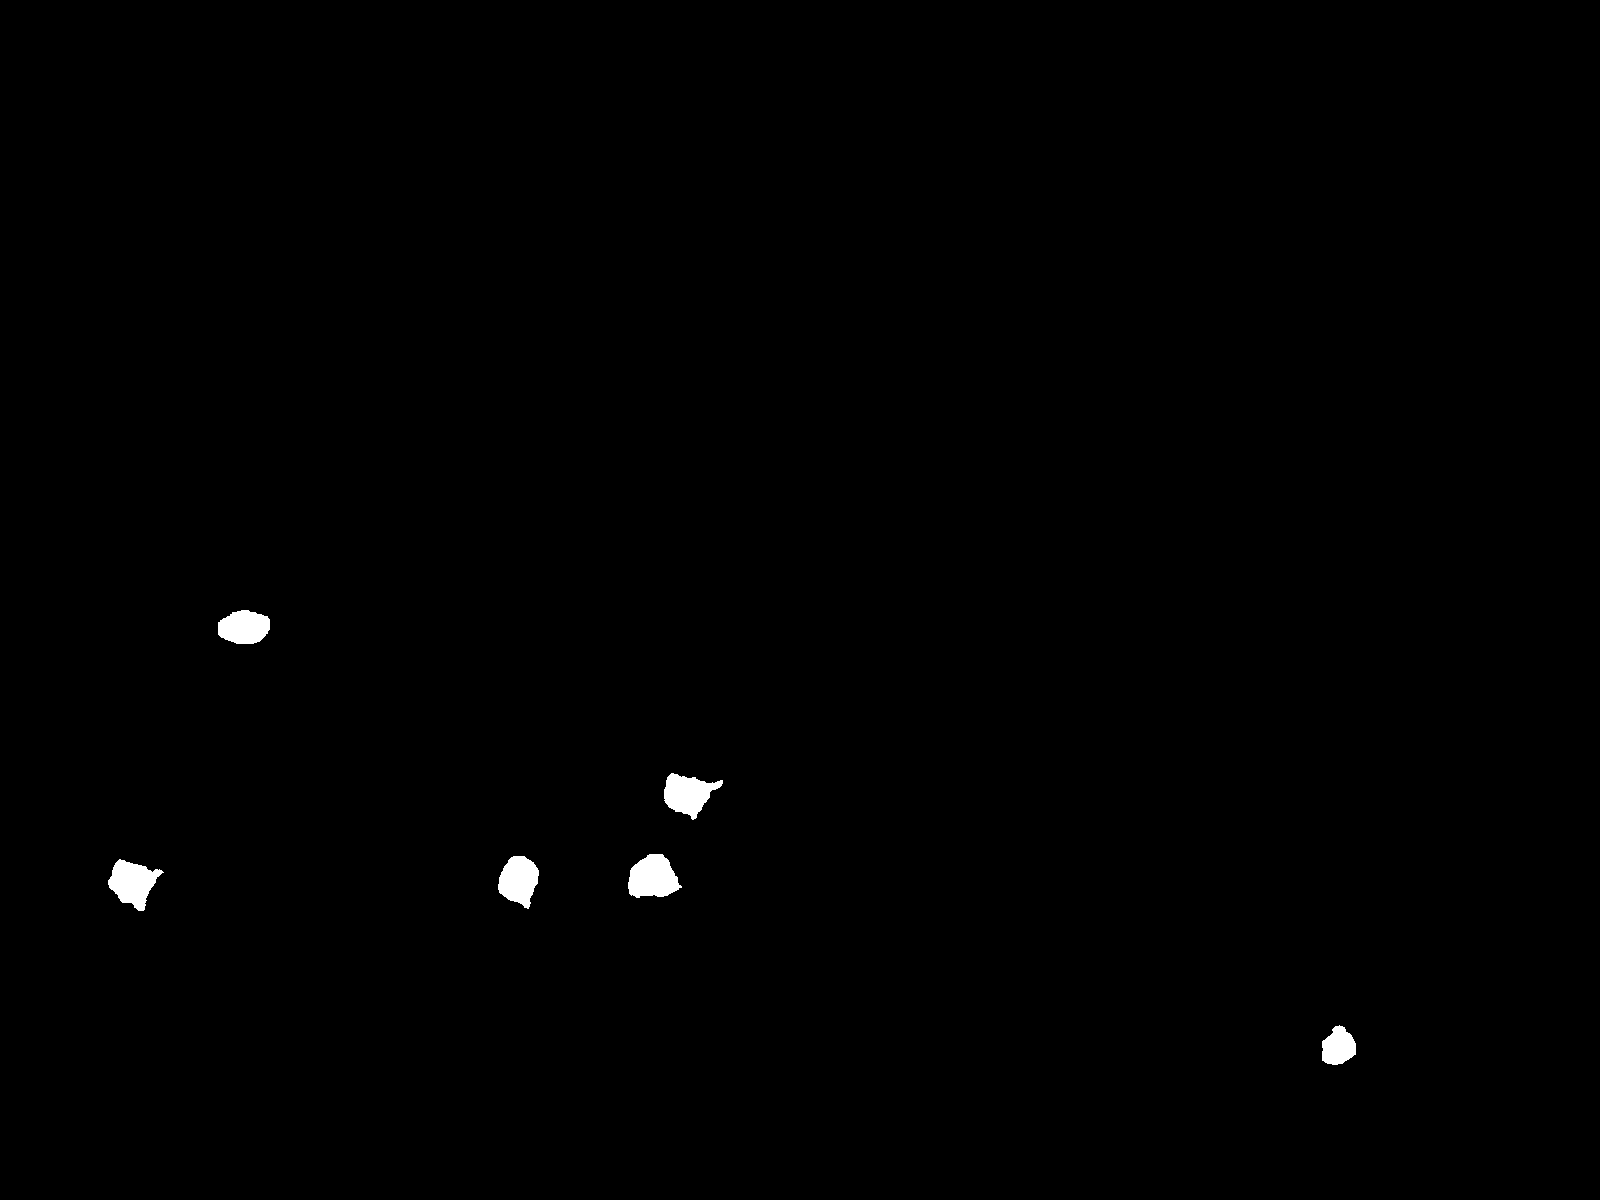
\includegraphics[width=0.5\linewidth]{figures/120_dataset/m_maccherone.png}
\subcaption{}
\label{fig:artifacts:macaroon}
\end{subfigure}
\vspace{-0.2cm}
\caption{
\textbf{Artifacts and challenges}. Neuronal cells appear of different shape, size and saturation over a background of variable brightness and color.
%%rephrase
% \textbf{Sample data}. In the original images (left), the neuronal cells of interest appear as yellow spots over a background of variable brightness and color. They exhibit a large variability in terms of shape, size and saturation, which makes them hard to distinguish from artifacts and similar biological structures that are not of interest.
% The corresponding ground-truth masks used for training (right) depicts cells as white pixels over a black background.
} 
\label{fig:artifacts}
\end{figure}

The \textbf{Fluorescent Neuronal Cells} dataset \cite{clissa2021fluocells} consists of 283 
% high-resolution 
pictures 
% (1600$\times$1200 pixels) 
of mice brain slices and the corresponding ground-truth labels.
In order to acquire these images, the mice were subjected to controlled experimental conditions, and a monosynaptic retrograde tracer (Cholera Toxin b, CTb) was surgically injected into brain tissues to highlight the neurons connected to the injection site
%projecting to the injection site
\cite{hitrec2019neural}.
Specimens of brain slices were then observed through  
a fluorescence microscope configured to select the narrow wavelength of light emitted by 
a fluorophore (of a yellow/orange color) associated with the tracer.
Thus, the resultant images depict neurons of interest as
% objects of different size and shape appearing as 
yellow-ish spots
% of variable brightness and saturation 
over a composite, generally darker background (\cref{fig:dataset,fig:artifacts}, left).

% Although many efforts were made to stabilize the acquisition procedure, the images present several relevant challenges for the detection task. 
% For example, the variability in brightness and contrast causes some fickleness in the pictures overall appearance (cf. \cref{fig:dataset:dark,fig:dataset:bright}).  
% Also, the cells themselves exhibit varying saturation levels due to the natural fluctuation of the fluorescent emission properties (cf. \cref{fig:dataset:dark,fig:artifacts:clumping}).
% Moreover, the substructures of interest have a fluid nature. This implies that the size and shape of the stained cells may change significantly (see \cref{fig:artifacts:clumping}, right), making it even harder to discriminate between them and the background. 
% Combined to that, artifacts (\cref{fig:artifacts:stripe,fig:artifacts:macaroon}), bright biological structures -- like neurons' filaments -- (\cref{fig:artifacts:stripe}) and non-marked cells similar to the stained ones handicap the recognition task. 
% Last but not least, another source of complexity is the broad shift in the number of target cells from image to image.
% Indeed, the total counts range from no stained cells (\cref{fig:dataset:empty}) to several dozens clumping together (\cref{fig:artifacts:clumping}). 
% As a consequence, this requires a model with both high precision -- to prevent false positives in the former case -- and high recall -- since considering two or more touching neurons only once produces false negatives.
% % In the former case, the model needs high precision in order to prevent false positives. The latter, instead,
% % requires high recall since considering two or more touching neurons only once produces false negatives. 

% By and large, all of these factors make the recognition and counting tasks more problematic and complicate the model training.
% Likewise, these challenges hinder model evaluation as the interpretation of such borderline cases becomes subjective.

\section{Ground-truth labels}
Under a supervised learning framework, the training phase leverages ground-truth labels acting as examples of desired outputs that the model should learn to reproduce. 
In the case of image segmentation, such targets are in the form of binary images (\textit{masks}) where the objects to segment and the background are represented by white and black pixels, respectively (Fig. \ref{fig:dataset}, right).

Obtaining target masks usually requires a great effort in terms of time and human resources, so an initial automatic procedure was exploited to speed up the labeling process. 
In particular, starting from a large subset composed by 252 pictures, gaussian blurring was first applied to mitigate small-frequency noise. 
Then, the resulting images were subjected to a thresholding operation.
% using a cutoff selected base on the pixel intensity histogram shape. 
For this step, the image histogram of the pixel intensity was considered, and a cutoff equal to the 97\emph{-th} percentile of the intensity distribution was adopted for binarization. 
The goal was to obtain a loose selection of good candidates to be labeled as neuronal cells. 
After that, acknowledged operators reviewed the results to discard the false positives introduced with the previous procedure, taking care of excluding irrelevant artifacts and misleading biological structures.
The remaining 31 images were segmented manually by domain experts. Significant pictures with peculiar traits -- such as artifacts, filaments and crowded objects -- were included in the latter set to have highly reliable masks for the most challenging examples\footnote{check the \emph{README} file in \citeA{clissa2021fluocells} for a detailed list of manually segmented images}. 
% (see $link_to_github$ for more details).

% \lc{A summary of the distributions of counts and objects features is presented in Table \ref{tab:dataset_summary}}.
% % ...possibly add geometrical information of cell objects, average/median/max/min counts per image, ... others(?)
% \begin{table}[b]
% \begin{center}
% \begin{tabular}{cccccc}
% \hline
% area    & minor axis & major axis & equivalent diameter & maximum feret diameter & mean diameter \\
% \hline
% 1206.43 & 29.39 & 50.43 & 36.50 & 55.34 & 47.42\\
% \hline
% \end{tabular}
% \caption{Summary statistics of cells morphological features (measured in pixels)}
% \label{tab:dataset_summary}
% \end{center}
% \end{table}


Despite the huge popularity Deep Learning has gained in computer vision in the last decade, the lack of annotated data is a common curse when dealing with applications involving non-standard pictures and/or tasks \cite{curse_dataset_annotation}. 
Since ground-truth labels are expensive to acquire in terms of time and costs \cite{vija2009annotationcost, mullen2019comparing}, a common approach is to fine-tune models pre-trained on giants datasets of natural images like ImageNet \cite{ImageNet} or COCO \cite{COCO}, possibly using as few new labels as possible for the task of interest. 
However, this strategy often does not apply to use cases where the pictures under analysis belong to extraneous domains with respect to the ones used for pre-training \cite{TL_medical_imaging}.
For this reason, by releasing the annotated dataset\footnote{\dataset} and the pre-trained model\footnote{\linkmodel} we hope to \textit{i)} foster advances in fields like biomedical imaging through the speed up guaranteed by the automation of manual operations, and \textit{ii)} promote methodological research on new techniques of data analysis for microscopic fluorescence and similar domains.


\section{Data exploration}
\label{sec:data_exploration}

Fluorescent Neuronal Cells images are high-resolution RGB pictures of constant shape (1200 pixels height by 1600 pixels width) collected under fixed experimental conditions.
% In terms of data features, the most interesting aspects regard the color and luminance information, the counts distribution and the cells characteristics.
% In terms of data features, the most interesting aspects pertain the color and luminance information, the counts' distribution and characteristics of the cells.
The data can be explored at two complementary levels: pixel features and cell characteristics. 
On the one hand, interesting insights can be retrieved by looking at pixels' color and luminance information. Also, analogous analyses on the ground-truth masks reveal essential information about class-imbalance between signal and background.
On the other hand, examining object properties can highlight potential nuisances and suggest how to evaluate model performances.

The above data explorations are presented in the following sections of this chapter, and a summary table of the most important data features is reported in \cref{tab:data_features}.
\renewcommand{\cellalign}{cc}
\renewcommand{\theadalign}{cc}
\begin{table}[]
    \centering
    \resizebox{\textwidth}{!}{
    % \begin{tabular}{lrrrrrrrr}
    % \toprule
    % {} &          \thead{red\\intensity} &        \thead{green\\intensity} &         \thead{blue\\intensity} &  signal (\%) &  signal ratio &     area &  \thead{Feret\\diameter} &  \# cells \\
    % \midrule
    % mean &   7.32 &   2.83 &  0.20 &        0.50 &    366,681.94 & 1,212.18 &           55.71 &    27.05 \\
    % \thead{standard\\deviation}  &  16.81 &  13.30 &  1.43 &        0.61 &    755,628.42 &   995.40 &           26.12 &    21.75 \\
    % min  &   0 &   0 &  0 &        0 &         19.57 &   162 &           18.68 &     0 \\
    % 10\%  &   0 &   0 &  0 &        0 &         92.39 &   358 &           30.02 &     4 \\
    % 25\%  &   2 &   0 &  0 &        0.09 &        145.35 &   564 &           38.08 &     7 \\
    % 50\%  &   5 &   1 &  0 &        0.34 &        291.10 &   913 &           49.50 &    21 \\
    % 75\%  &   9 &   2 &  0 &        0.68 &      1,163.29 & 1,504 &           66.48 &    48 \\
    % 90\%  &  12 &   4 &  0 &        1.07 &  1,920,000 & 2,409 &           88.02 &    59 \\
    % max  & 252 & 251 & 87 &        4.86 &  1,920,000 & 8,092 &          215.10 &    68 \\
    % \bottomrule
    % \end{tabular}
    
    \begin{tabular}{lrrrrrrrr}
    \toprule
    {} &          \thead{red\\intensity} &        \thead{green\\intensity} &         \thead{blue\\intensity} &  signal (\%) &  signal ratio &     area &  \thead{Feret\\diameter} &  \# cells \\
    \midrule
    count & 1,919,905 & 1,919,910 & 1,919,955 &      283 &        283 & 2,137 &        2,137 & 2,193 \\
    mean  &         7.32 &         2.83 &         0.20 &        0.50 &    366,681.94 & 1,212.18 &           55.71 &    27.05 \\
    \thead{standard\\deviation}   &        16.81 &        13.30 &         1.43 &        0.61 &    755,628.42 &   995.40 &           26.12 &    21.75 \\
    min   &         0 &         0 &         0 &        0 &         19.57 &   162 &           18.68 &     0 \\
    10\%   &         0 &         0 &         0 &        0 &         92.39 &   358 &           30.02 &     4 \\
    25\%   &         2 &         0 &         0 &        0.09 &        145.35 &   564 &           38.08 &     7 \\
    50\%   &         5 &         1 &         0 &        0.34 &        291.10 &   913 &           49.50 &    21 \\
    75\%   &         9 &         2 &         0 &        0.68 &      1,163.29 & 1,504 &           66.48 &    48 \\
    90\%   &        12 &         4 &         0 &        1.07 &  1,920,000 & 2,409 &           88.02 &    59 \\
    max   &       252 &       251 &        87 &        4.86 &  1,920,000 & 8,092 &          215.10 &    68 \\
    \bottomrule
    \end{tabular}
    }
    \caption{\textbf{Distributions summary.} 
    Summary of the distributions illustrated in \cref{sec:data_exploration}. For each distribution we report the mean and standard deviation; minimum, maximum and 10\textit{-th}, 25\textit{-th}, 50\textit{-th}, 75\textit{-th} and 90\textit{-th} percentiles; the count of objects from which such measures are computed, i.e. pixels, images and cells.
    Notice that \textit{\# cells} count is obtained from the 2137 cells plus the 56 empty images.
    % Notice that commas are used as thousands separator
    }
    \label{tab:data_features}
\end{table}

\subsection{Salient features}
\label{sec:data_features}

% As far as the color, t
The picture appearance is dominated by two prevalent tints due to the intentional selection of a specific wavelength: a darker hue corresponding to areas whose light was filtered out and a yellow tone emitted by the fluorophore
(\cref{fig:dataset:empty,fig:artifacts}).
As a consequence, the only color channels to be populated are red and green, while blue is typically empty. 
An example of this effect is reported in \cref{fig:dataset:pixel_intensity}, where the average distribution of pixel intensity is illustrated (log scale).
\begin{figure}
    \centering
    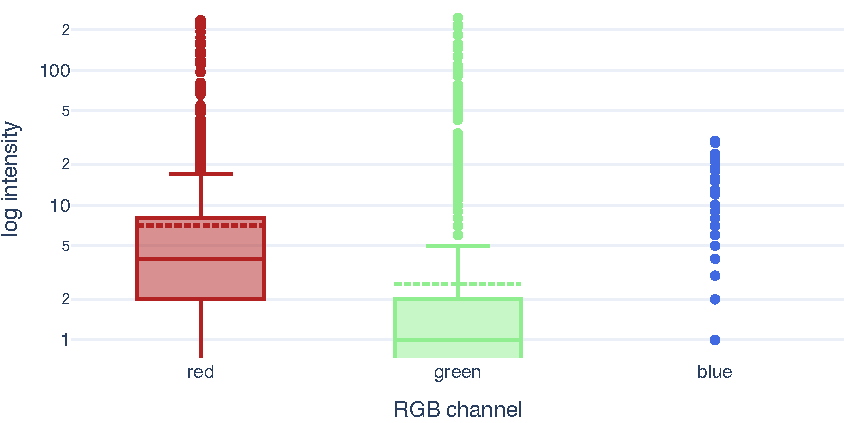
\includegraphics[width=\textwidth]{figures/120_dataset/features/pixel_intensity_distribution.pdf}
    \caption{\textbf{Pixel intensity distribution.} Violin plot of the average distribution of pixel intensities across the  RGB channels}
    \label{fig:dataset:pixel_intensity}
\end{figure}
In practice, the blues have an extremely narrow distribution squashed on zero, which makes it even difficult to visualize -- in fact only outliers are visible. 
The red and green channels are instead more populated. Their central tendency is still concentrated on low values due to the prevalence of background pixels, however we observe longer and thicker right tails, especially for the red channel (see \textit{red}, \textit{green} and \textit{blue} columns in \cref{tab:data_features} for a numeric summary).
Guided by this observation, one may argue that all this information is superfluous, so resorting to a grayscale transformation could be better since the images are ultimately shades of yellow.
A nice way to visually investigate such relationships is by exploring the colorspace representations of several images.
\Cref{fig:dataset:colorspace} reports the RGB and HSV encodings for two randomly sampled images.
Indeed, the RGB representations (\cref{fig:dataset:colorspace:rgb1,fig:dataset:colorspace:rgb2}) corroborate the previous intuition, as most pixels lay almost on a straight line in the red-green plane. 
This suggests that the two channels are highly correlated, so a one-dimensional subspace may be enough to represent most of the variability of the data.
In turn, this would bring two advantages: ease the learning process -- as neural networks typically suffer when inputs are correlated %\cite{} 
-- and make it more efficient -- as only one channel is considered instead of three.

However, the use-case at hand has no stringent requirements in terms of computing resources and runtime, so the 3-channels training is still feasible.
More importantly, the information thrown away when converting to grayscale, although tiny, may be crucial to discriminate background and signal. 
Hence, a 3D-encoding may still be worthed but the RGB colorspace may not be the optimal representation to learn this separation. A hint of that is demonstrated in \cref{fig:dataset:colorspace:hsv1,fig:dataset:colorspace:hsv2}, where the same images are depicted according to the HSV encoding. 
In this case, the separation between dark and colored tones appears more evident. 
Moreover, most of the pixels are concentrated in low hue values
and their distribution seems more spread across the saturation-value plane. 

All that being considered, we try to leverage the insights of both approaches. 
On one side, the RGB colorspace is taken as a starting point to retain all available information. On the other, the model first layer is designed to incorporate a colorspace transformation from RGB to a single channel.
% In this way, the intent is to avoid introducing any colorspace-related bias by letting the model learn the most convenient representation and, at the same time, benefit from the computational advantage due to a lower dimensionality.
% The intent is to avoid introducing any colorspace-related bias by letting the model learn the most convenient representation without ignoring the fact that a one-dimensional manifold is probably enough to express the variability of the data.
% The intent is to avoid introducing any colorspace-related bias by letting the model learn the most convenient representation.
% At the same time, by forcing the learned encoding to one dimension, we do not ignore the observation that a one-dimensional manifold is probably enough to express the data variability.
In this way, we avoid introducing any colorspace-related bias since the model learns the most convenient representation.
At the same time, we exploit the observation that a one-dimensional manifold is probably enough to express the data variability by forcing the learned encoding to one channel.
% \begin{figure}
%     \centering
%     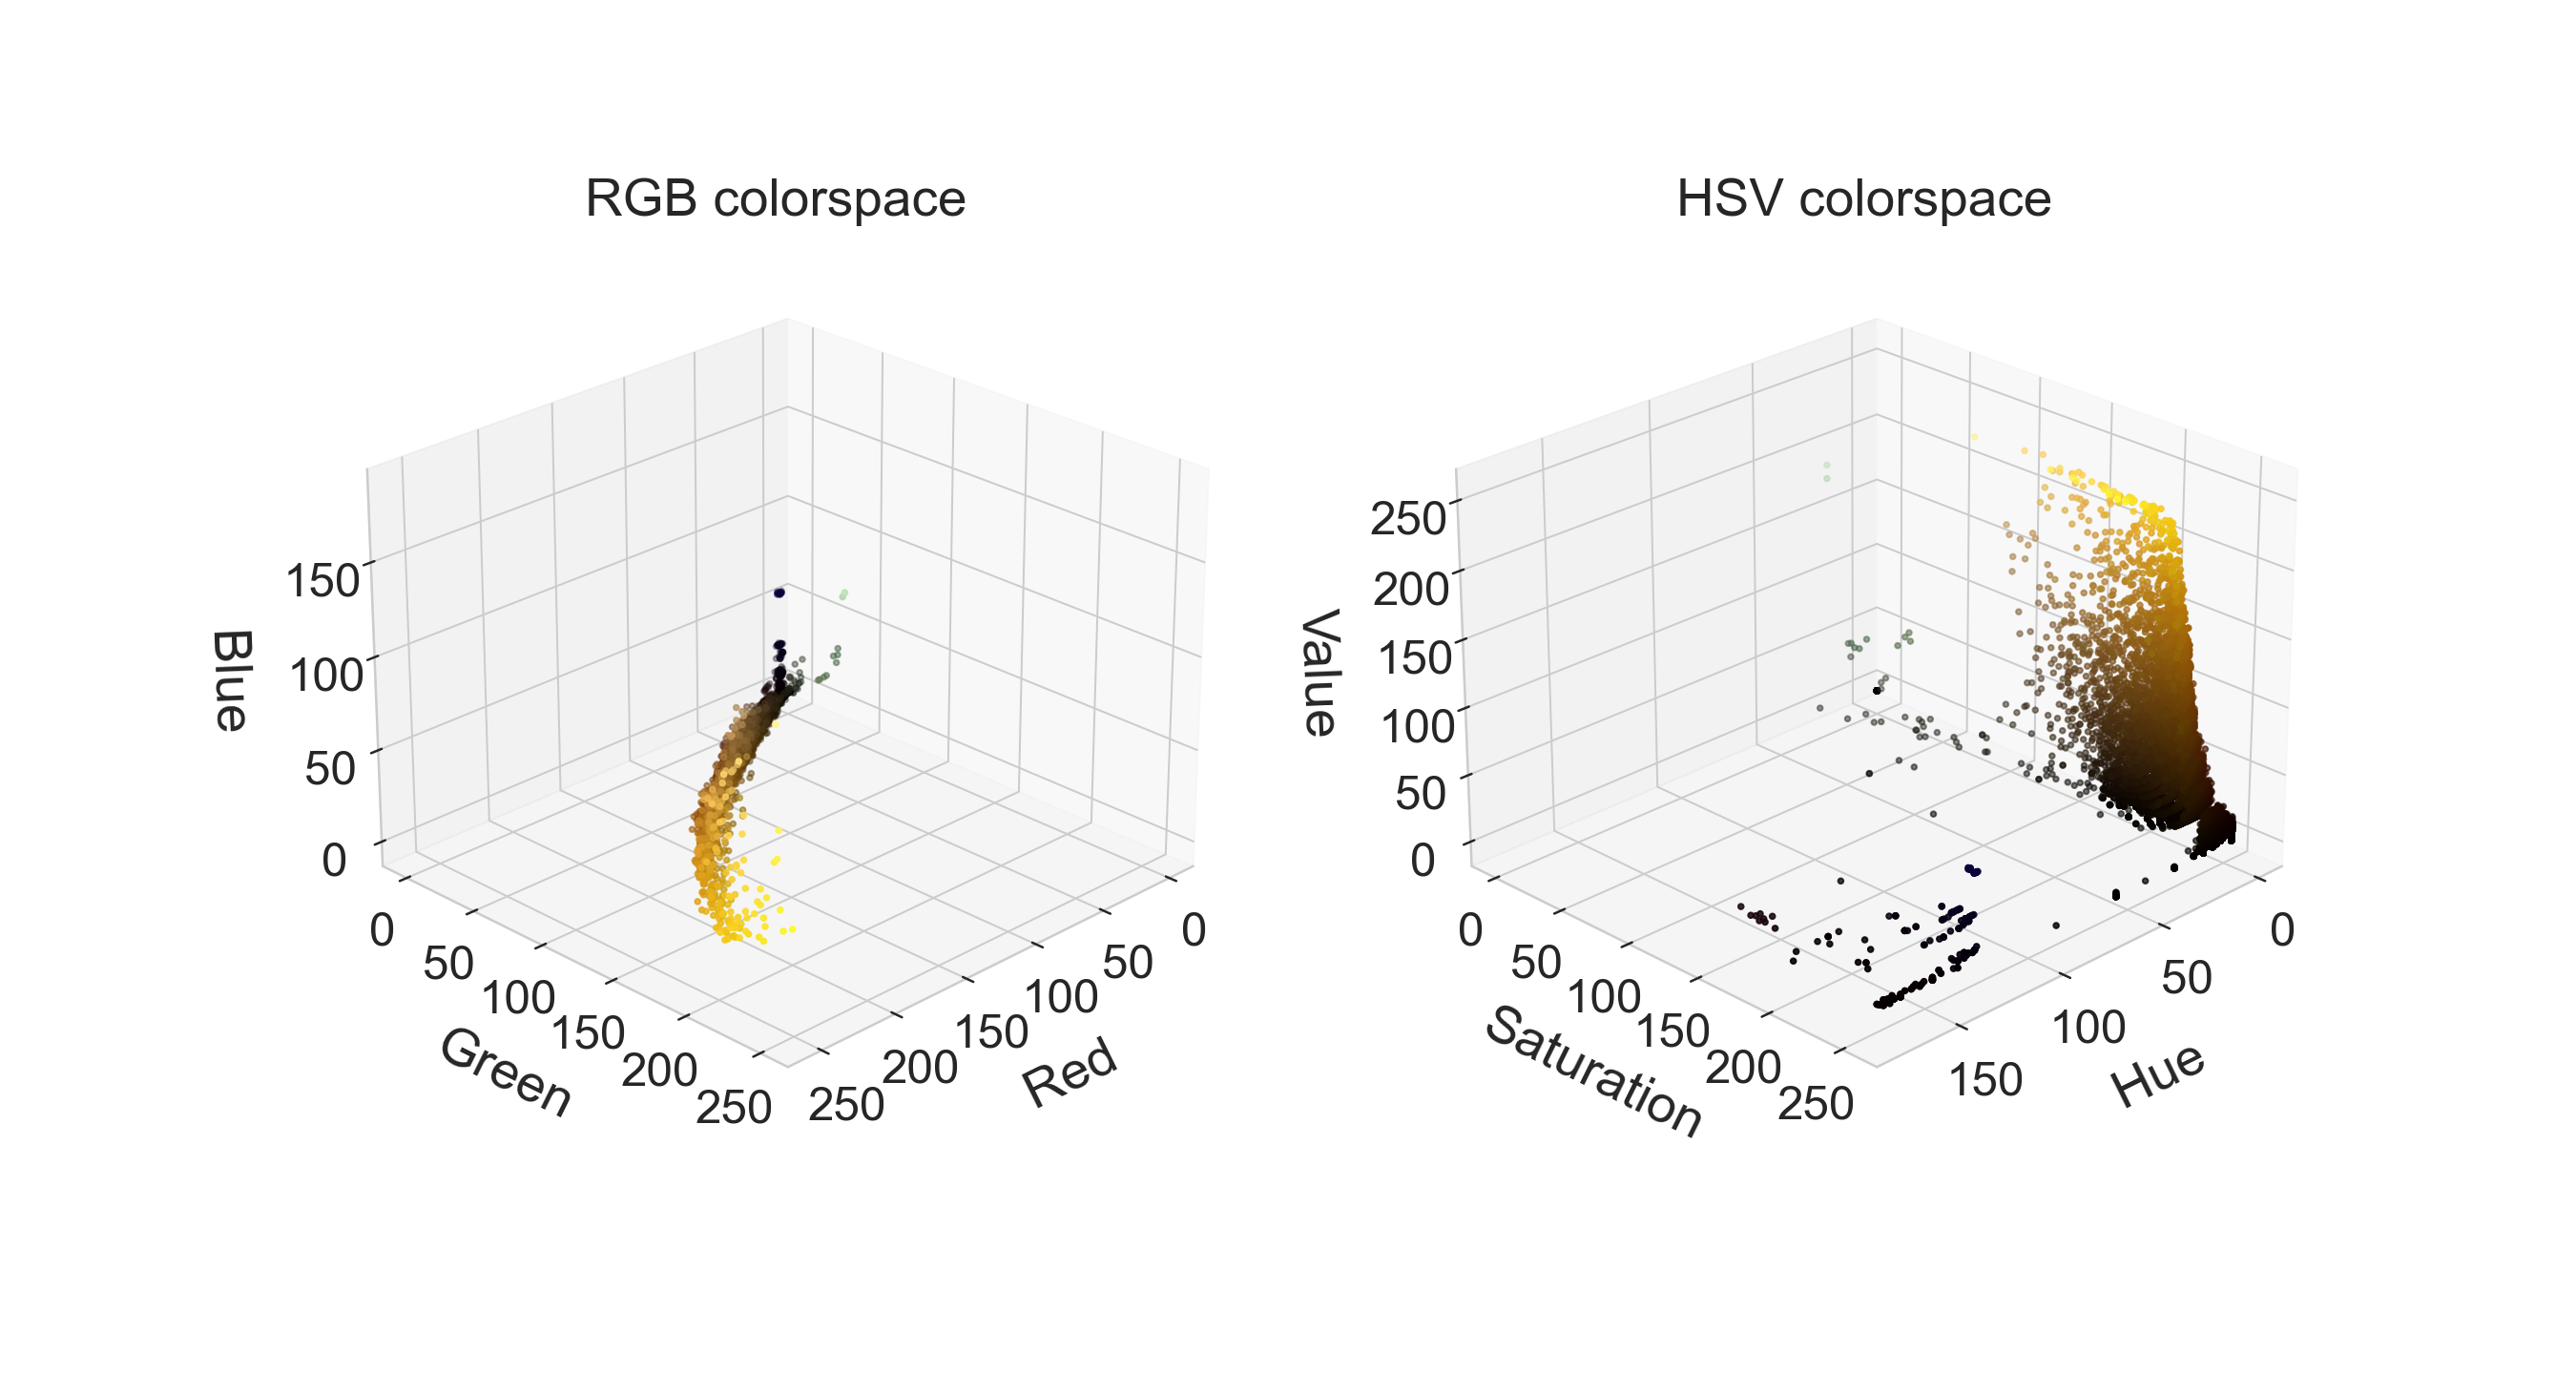
\includegraphics[width=1.1\textwidth]{figures/120_dataset/colorspace_Mar23bS1C2R3_VLPAGl_200x_y.png}
    
%     \centering
%     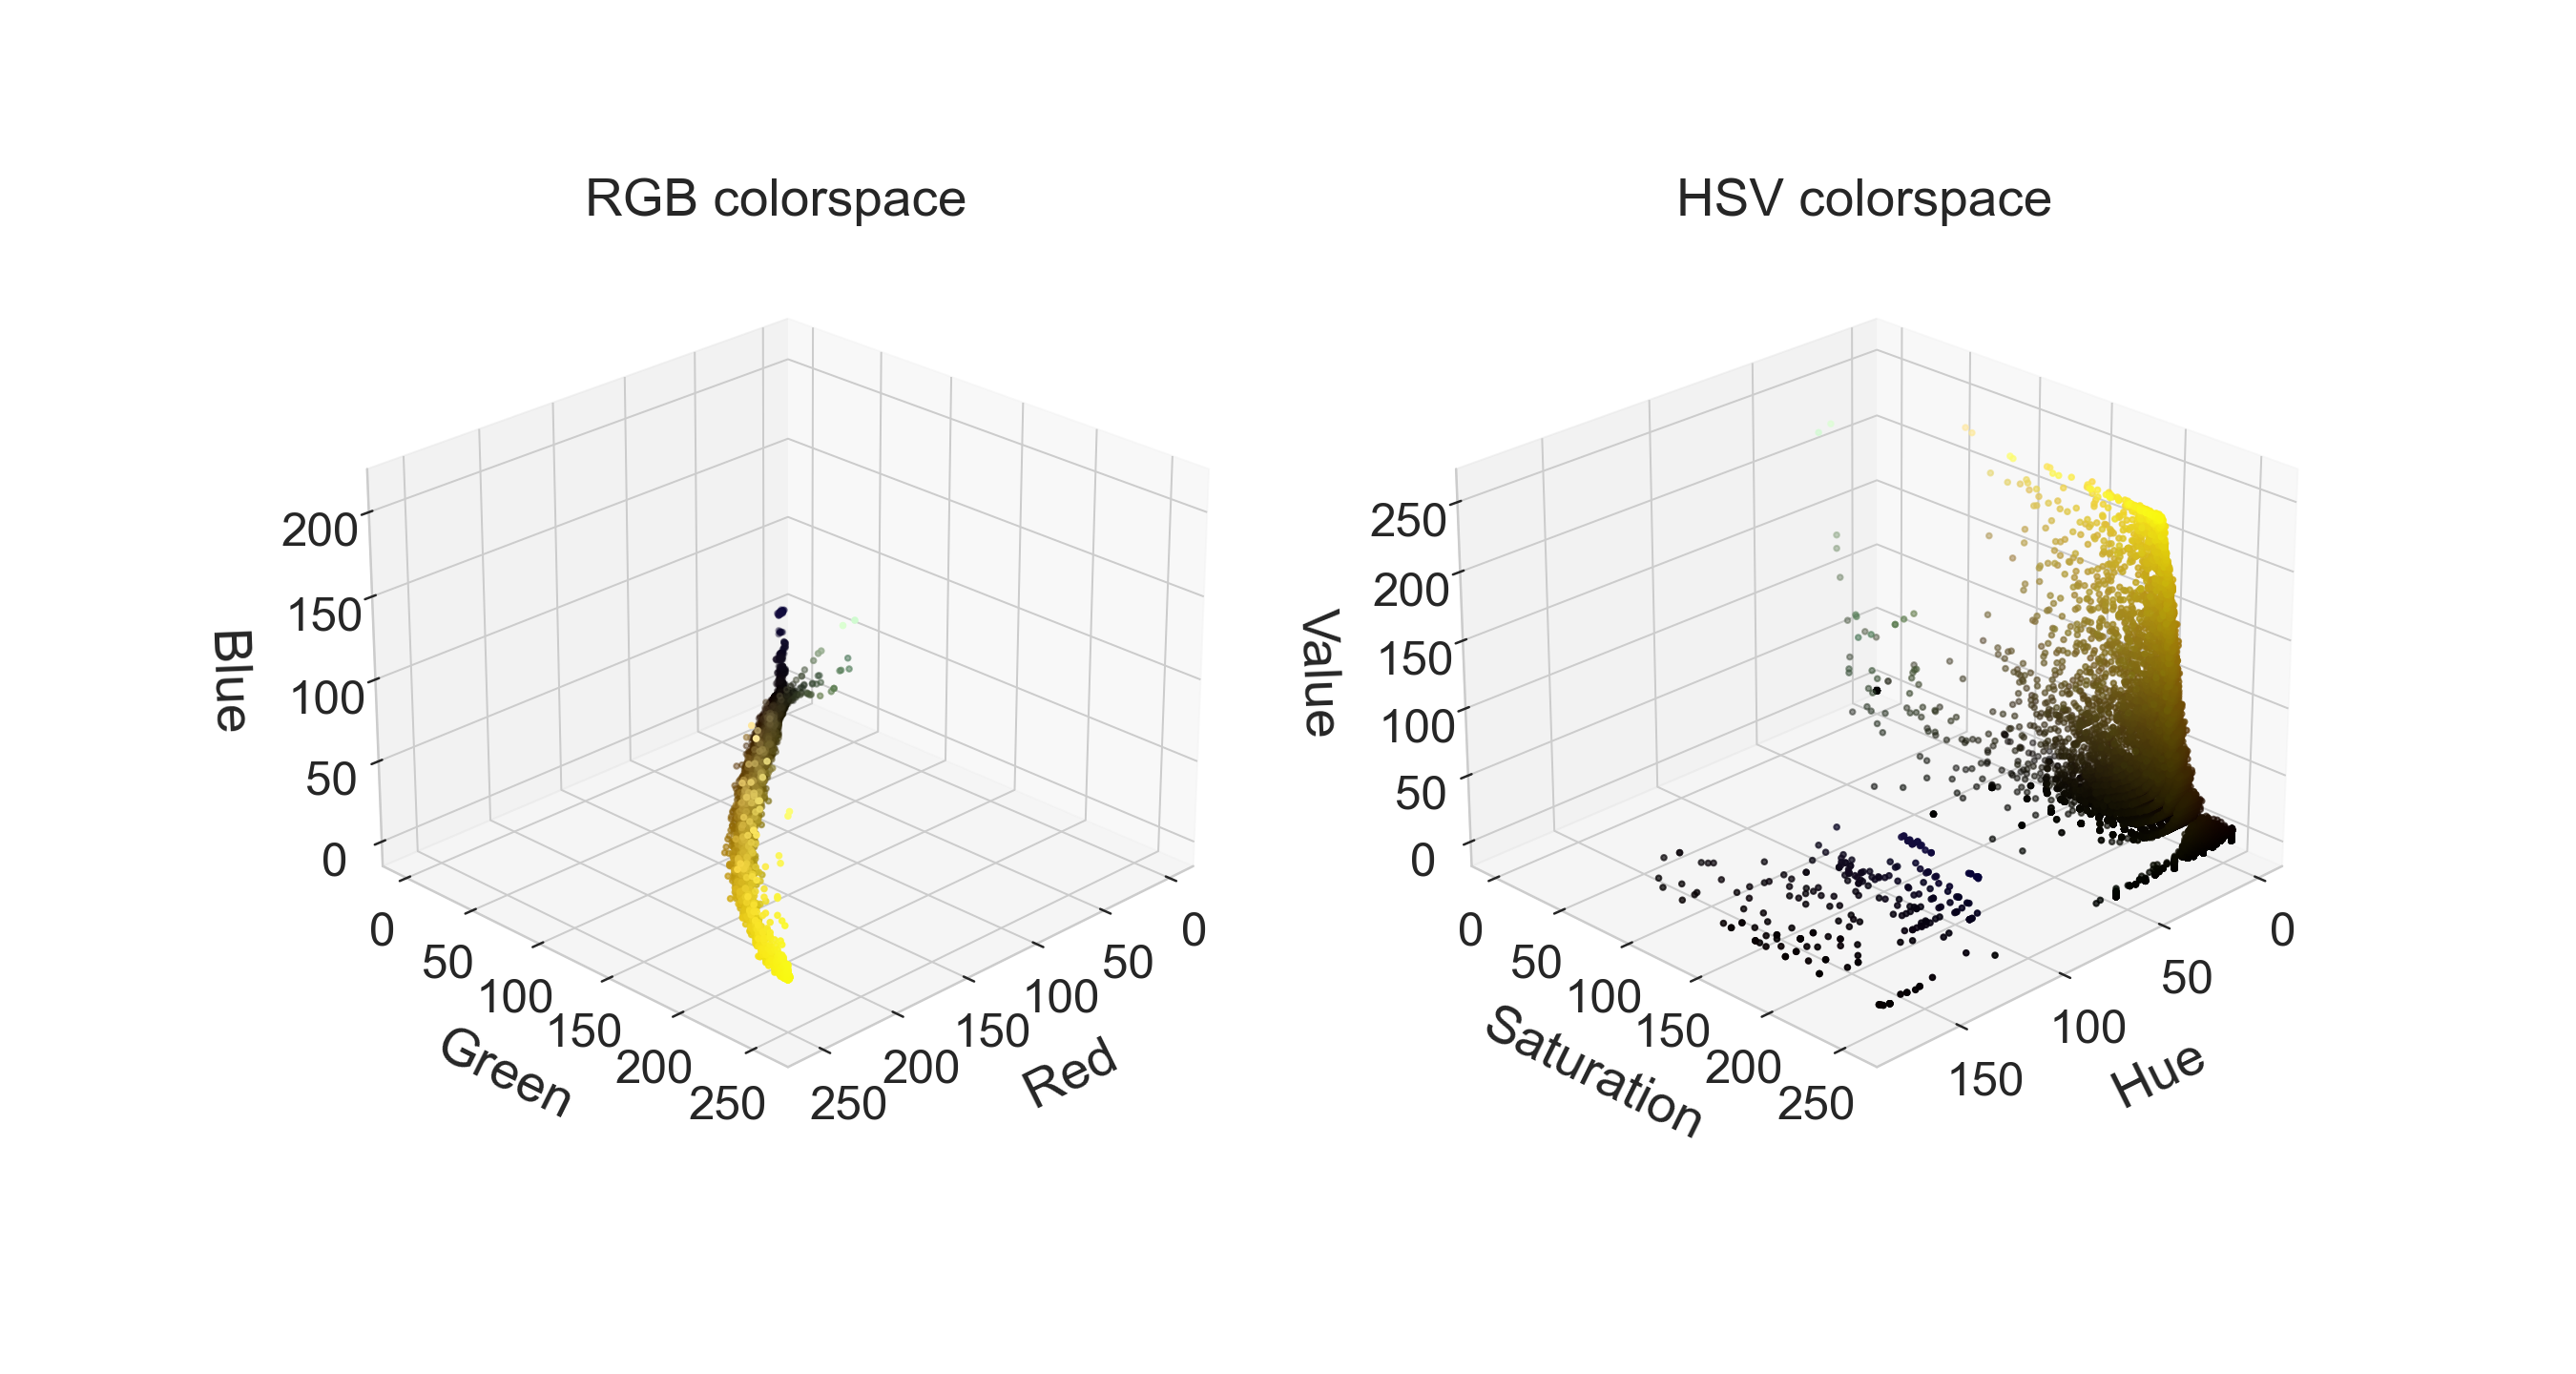
\includegraphics[width=1.1\textwidth]{figures/120_dataset/colorspace_Mar26bS2C1R2_DMl_200x_y.png}
%     \caption{Colorspace representation. The same image is represented as RGB (left) and HSV (right). Pixels are treated as 3D points with coordinates given by their encoding in the corresponding colorspace}
%     \label{fig:dataset:colorspace}
% \end{figure}
% \savegeometry{origigeom}
% \clearpage
% \newgeometry{lmargin=0.5cm}
\begin{figure}

    \centering
    Mar19bS1C4R3\_LHl\_200x\_y.png
    % \vspace{-3cm}
    \makebox[\textwidth][c]{\subfloat[RGB]{
    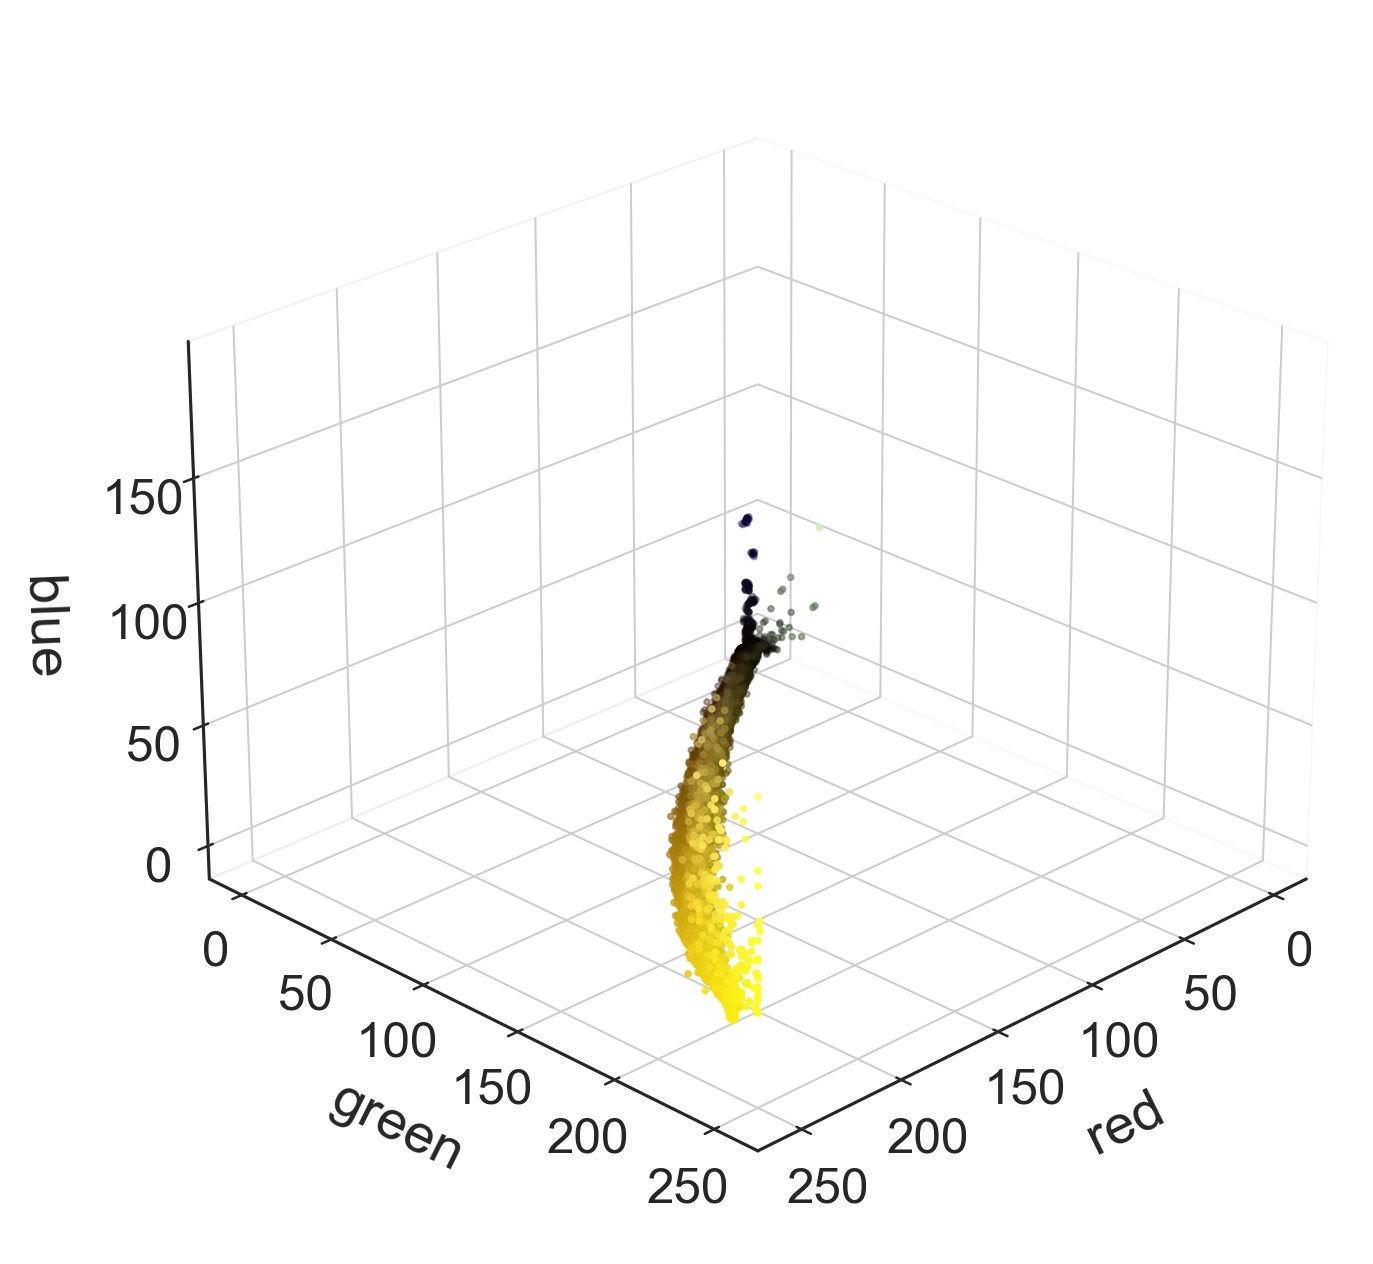
\includegraphics[width=0.55\textwidth]{figures/120_dataset/RGB_Mar19bS1C4R3_LHl_200x_y.png}\label{fig:dataset:colorspace:rgb1}
    }
    \subfloat[HSV]{
    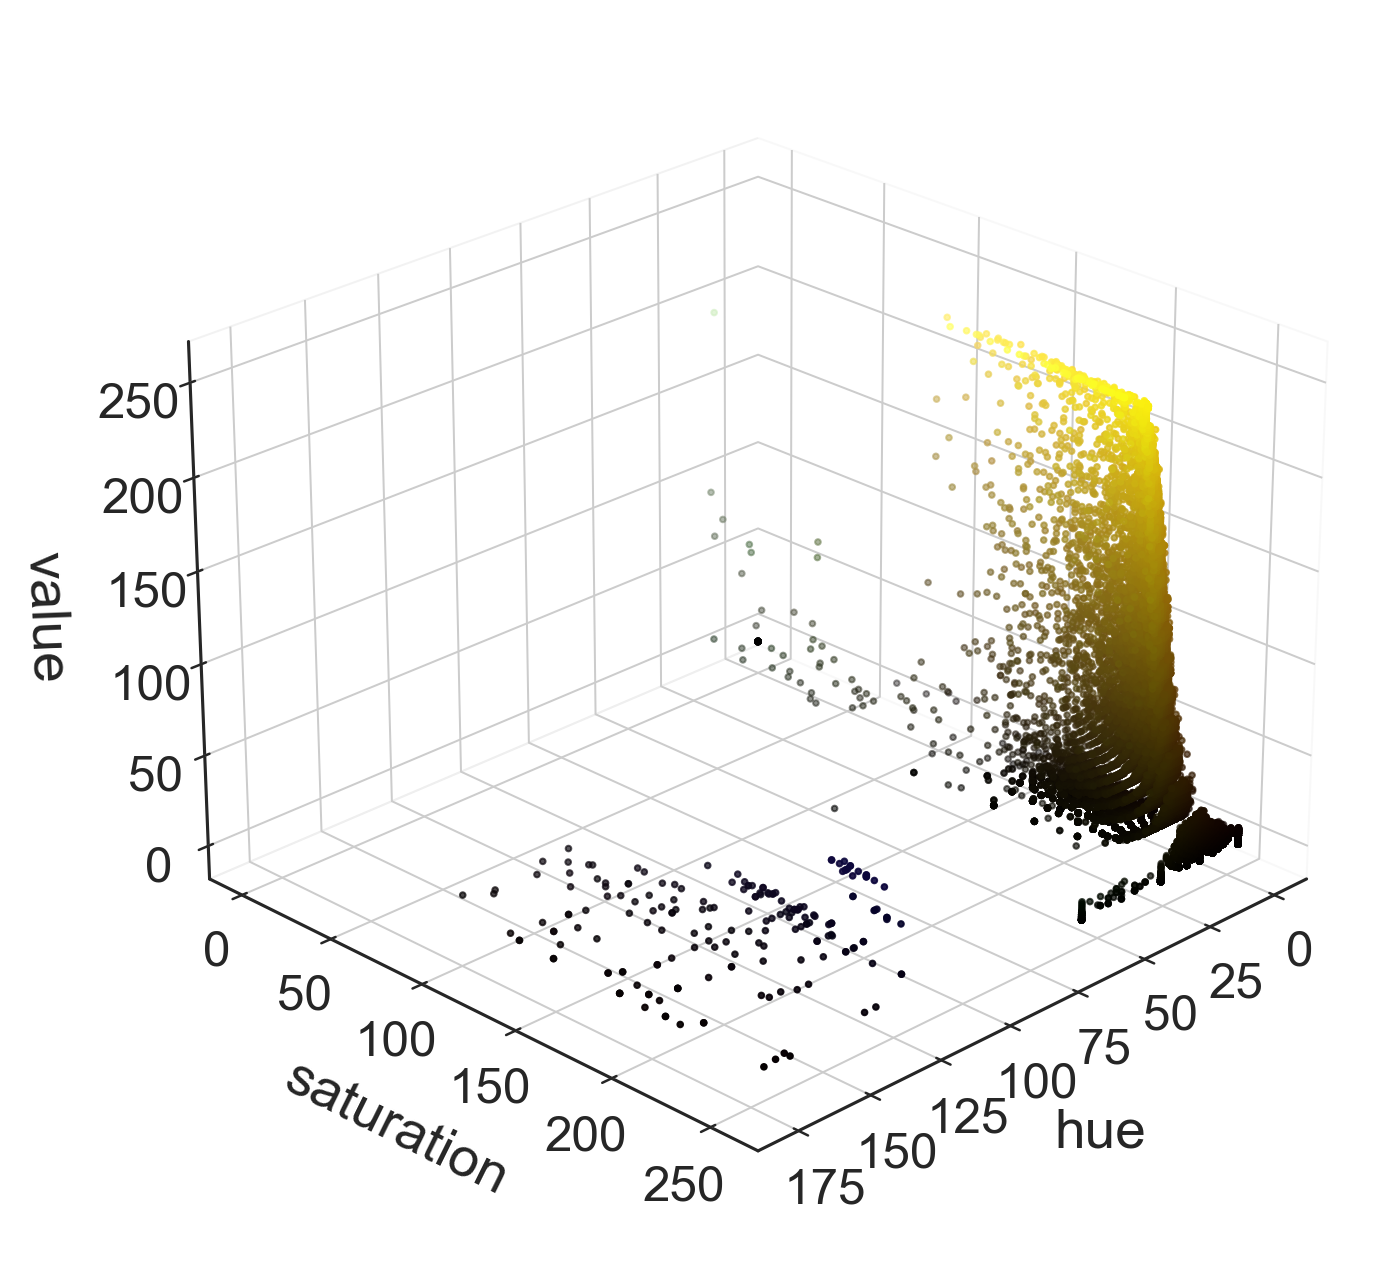
\includegraphics[width=0.55\textwidth]{figures/120_dataset/HSV_Mar19bS1C4R3_LHl_200x_y.png}\label{fig:dataset:colorspace:hsv1}
    }}
    
    \centering
    \vspace{1.5cm}
    Mar21bS1C1R3\_VLPAGl\_200x\_y.png   \makebox[\textwidth][c]{ \subfloat[RGB]{
    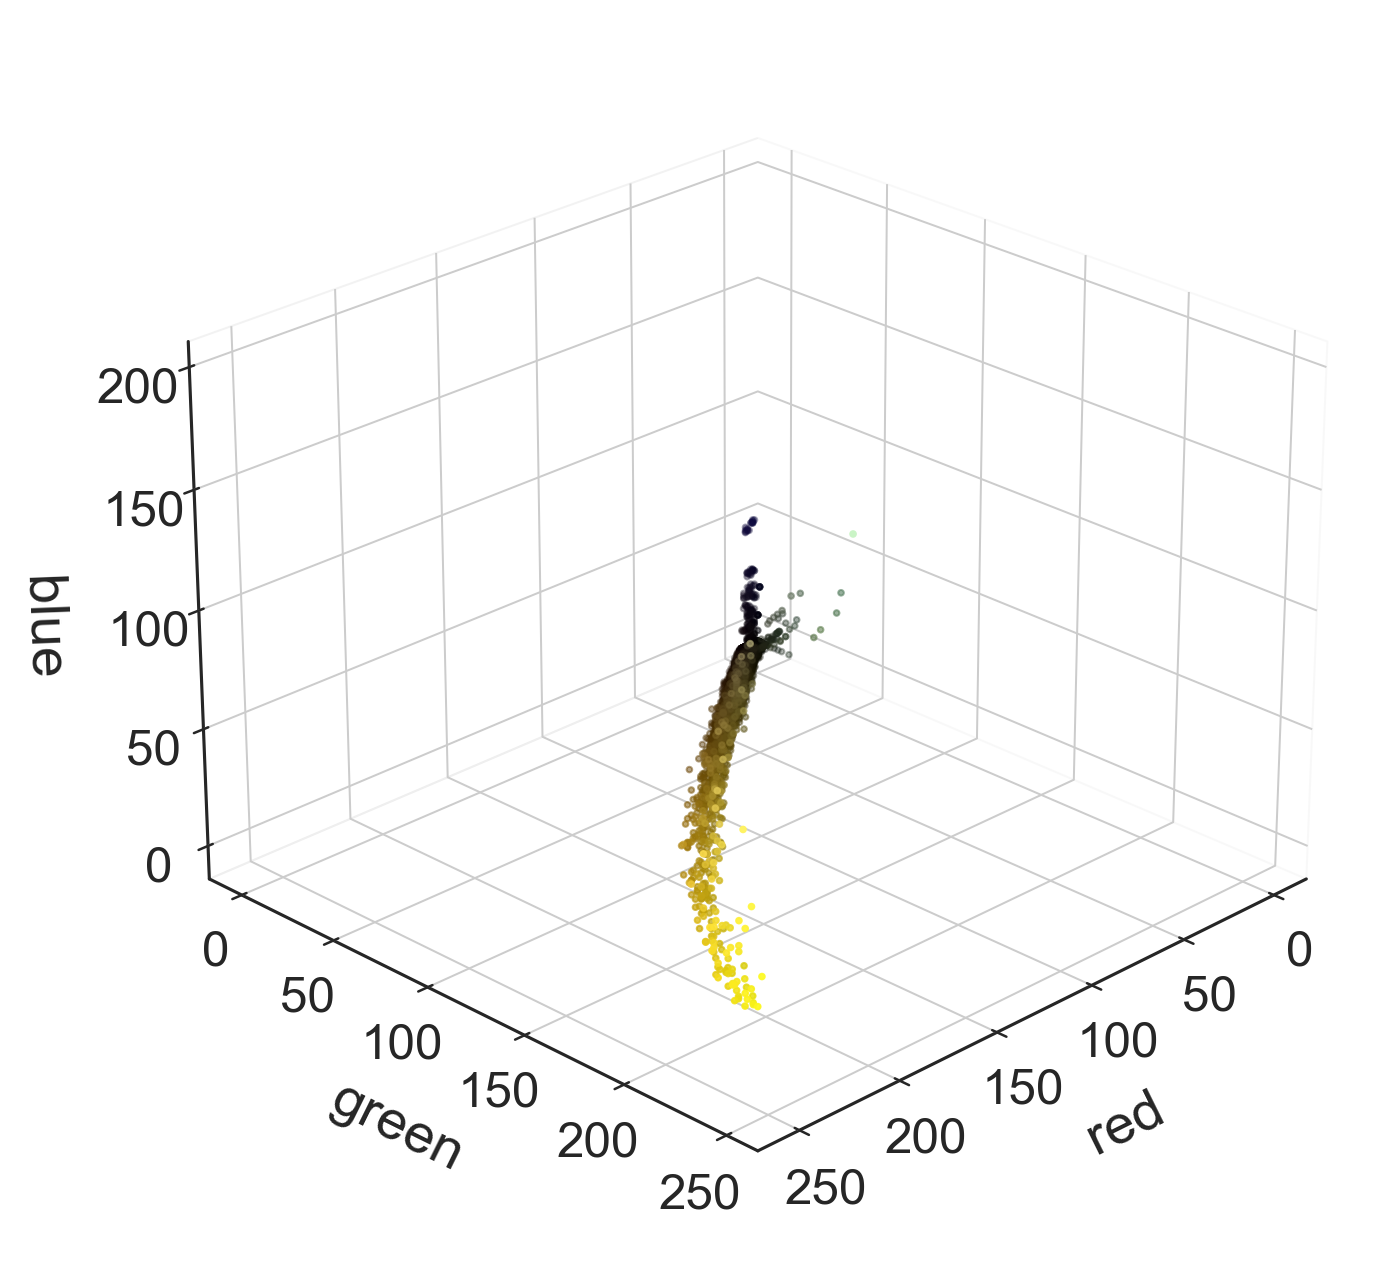
\includegraphics[width=0.55\textwidth]{figures/120_dataset/RGB_Mar21bS1C1R3_VLPAGl_200x_y.png}\label{fig:dataset:colorspace:rgb2}
    }
    \subfloat[HSV]{
    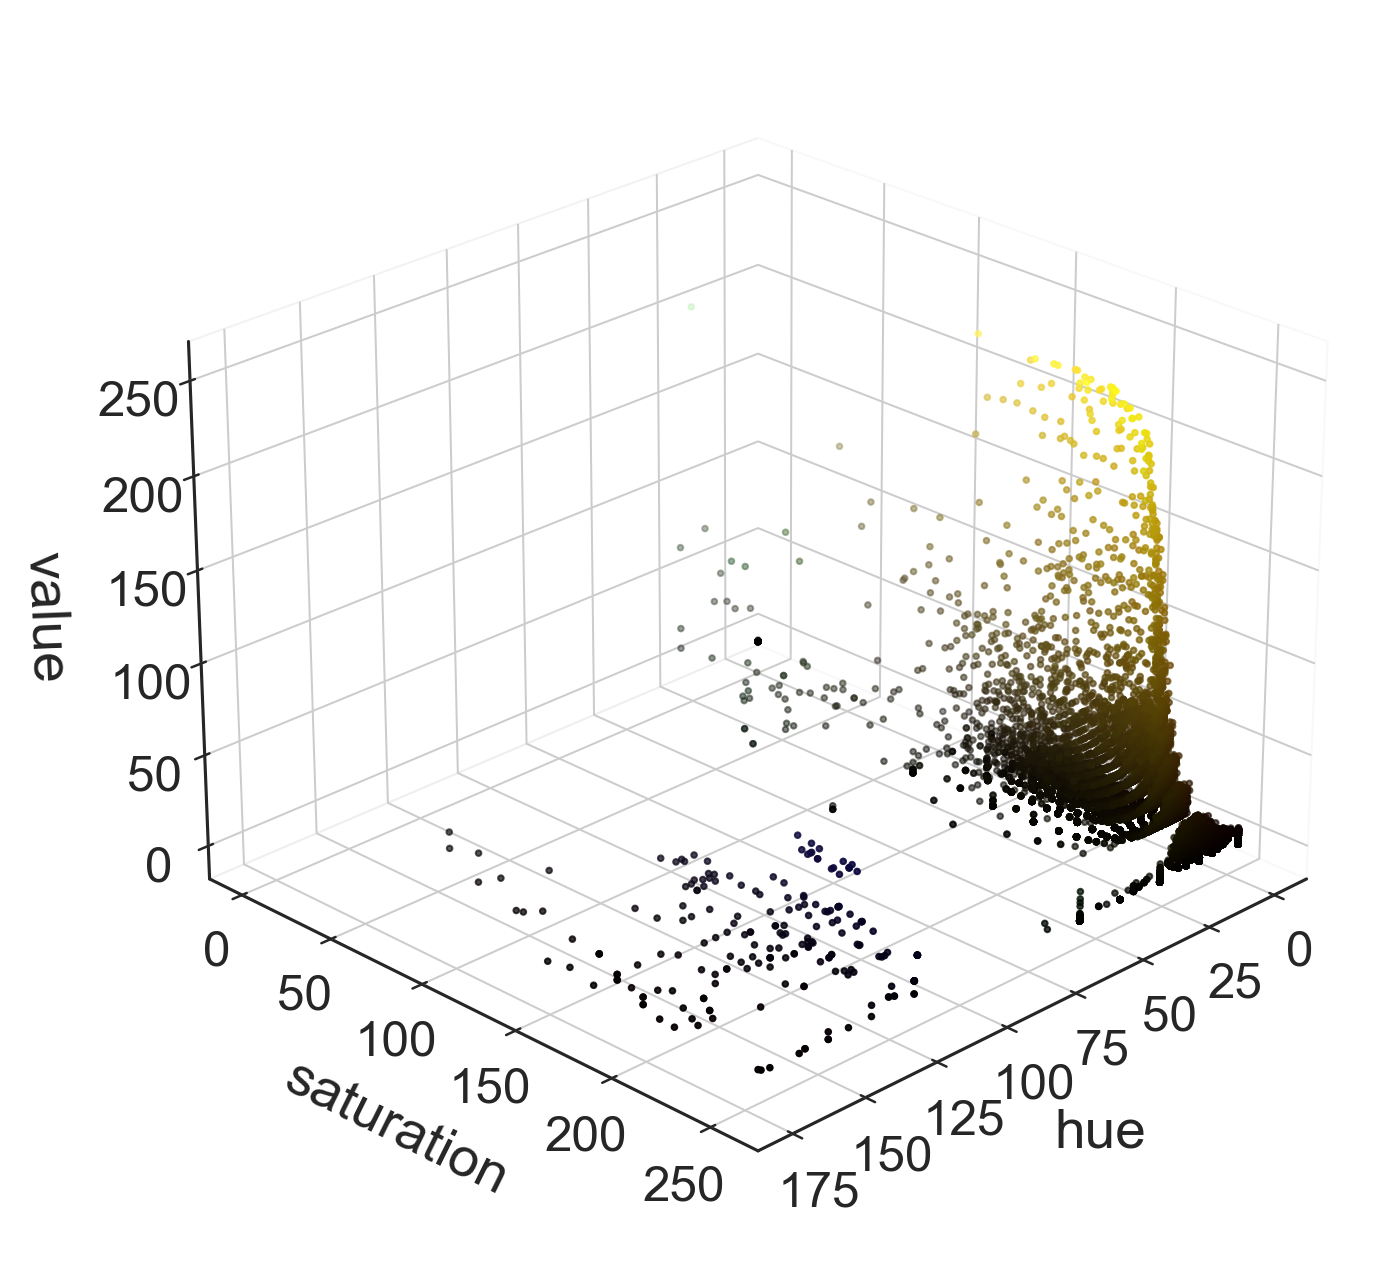
\includegraphics[width=0.55\textwidth]{figures/120_dataset/HSV_Mar21bS1C1R3_VLPAGl_200x_y.png}\label{fig:dataset:colorspace:hsv2}
    }}
    \caption{\textbf{Colorspace.} Two images represented as 3D points according to their RGB (left) and HSV (right) encodings. 
    Each point is colored as the corresponding pixel in the original image
    % The point color is the same as the pixel's color in the original image.
    }
    \label{fig:dataset:colorspace}
\end{figure}

% \clearpage
% \restoregeometry

\subsection{Class imbalance}
\label{sec:class_imbalance}
% \begin{figure}
%     \centering
%     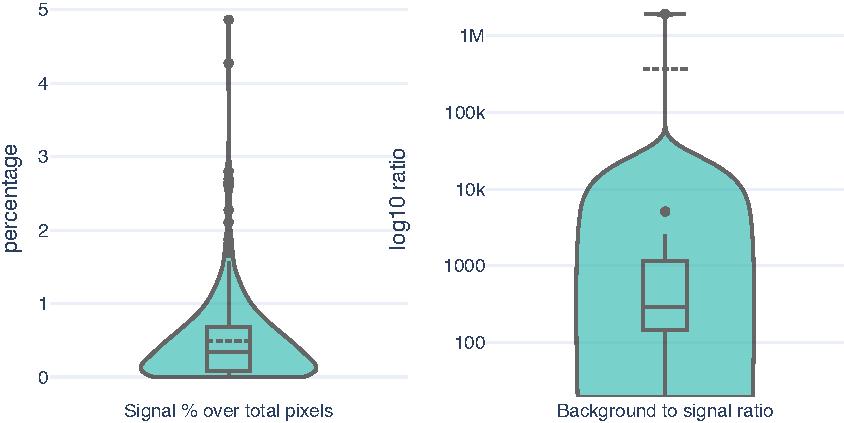
\includegraphics[width=\textwidth]{figures/120_dataset/features/class_imbalance.pdf}
%     \caption{\textbf{Class imbalance.} Violin plot and boxplot of signal percentage (left) and background to signal ration (right).}
%     \label{fig:dataset:class_imbalance}
% \end{figure}
\begin{figure}
    \centering
    \subfloat[Signal \% over total pixels]{
    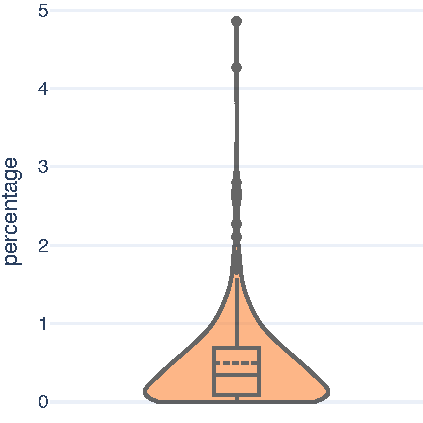
\includegraphics[width=0.5\textwidth]{figures/120_dataset/features/class_imbalance_percentage.pdf}\label{fig:dataset:class_imbalance:percentage}
    }
    \subfloat[Background to signal ratio]{
    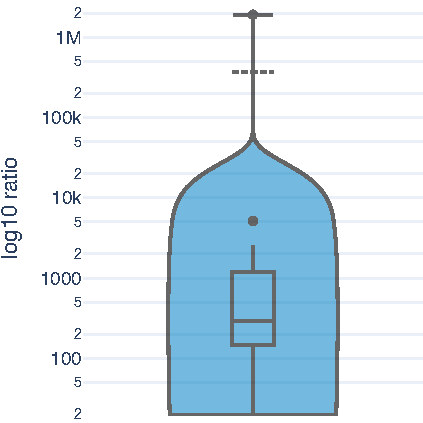
\includegraphics[width=0.5\textwidth]{figures/120_dataset/features/class_imbalance_ratio.pdf}\label{fig:dataset:class_imbalance:ratio}
    }
    \caption{\textbf{Class imbalance.} Violin plot and boxplot of signal percentage (left) and background to signal ration (right).}
    \label{fig:dataset:class_imbalance}
\end{figure}

Inspecting ground-truth masks at pixel level reveals important characteristics that affect the training process. 
By looking at the cardinality of pixels belonging to the background and the signal it is possible to notice how the two classes are extremely unbalanced (see \textit{signal (\%)}, and \textit{signal ratio} columns in \cref{tab:data_features} for a numeric summary).
\Cref{fig:dataset:class_imbalance:percentage} shows a violin plot of the percentage of signal pixel over the total image pixels across the 283 pictures.
The distribution is deeply skewed towards 0, with a median of 0.34\% and a 90\emph{-th} percentile of 1.07\%. 
Hence, almost 90\% of the images contain less than 1\% of pixels belonging to the signal%
% , causing an extreme unbalance between signal and background classes
.
Even more significantly, the right tail does not exceed 5\% of signal coverage, with a maximum of 4.86\%.

\Cref{fig:dataset:class_imbalance:ratio} illustrates the same concept but focuses on the relative proportion of background to signal. 
The distribution is left-skewed, with a lower half concentrated in the range (19, 291), i.e. background pixels are roughly from 20 to 300 times the signal pixels in 50\% of the images.
Remarkably, the disproportion grows even faster in the right tail, where the ratio explodes up to over 1000. 
Finally, notice that the bulk of outliers accumulates in the higher end of the domain. 
This is caused by the contribution of empty masks that cover more than 10\% of the total images.

These considerations expose the need for dedicated training strategies to face this strong class imbalance and correctly learn to classify image pixels.

\subsection{Objects features}
% \begin{figure}
%     \centering
%     \subfloat[Area]{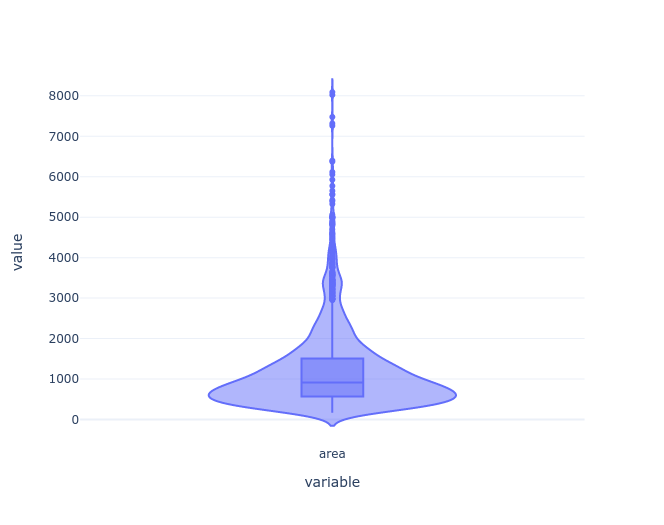
\includegraphics[width=0.5\textwidth]{figures/120_dataset/geometric_features area.png}
%     \label{fig:dataset:geom:area}
%     }
%     \subfloat[Feret diameter]{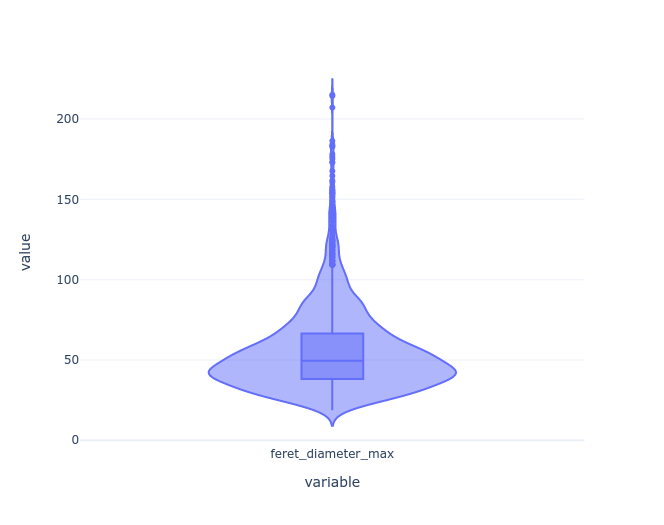
\includegraphics[width=0.5\textwidth]{figures/120_dataset/geometric_features feret.png}
%     \label{fig:dataset:geom:feret}
%     }
%     \caption{\textbf{Geometrical features.} Distributions of the area (left) and maximum Feret diameter (right) across all annotated cells.}
%     \label{fig:dataset:geom}
% \end{figure}
\begin{figure}
    \centering
    \subfloat[Area]{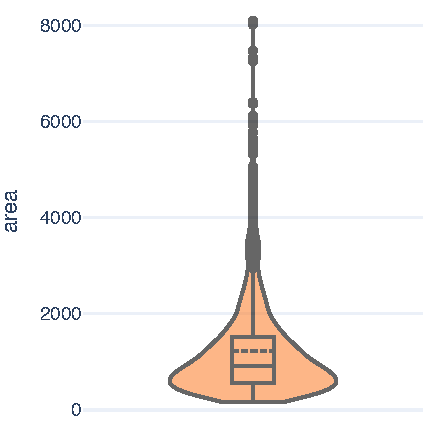
\includegraphics[width=0.5\textwidth]{figures/120_dataset/features/area.pdf}
    \label{fig:dataset:geom:area}
    }
    \subfloat[Feret diameter]{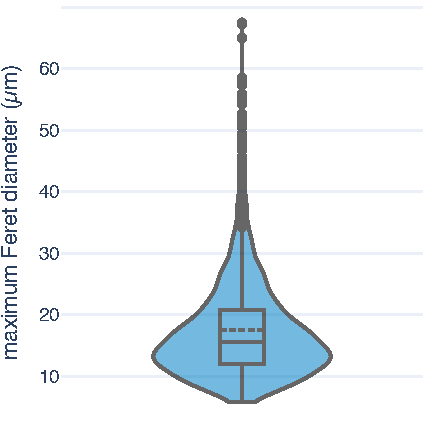
\includegraphics[width=0.5\textwidth]{figures/120_dataset/features/feret_diameter.pdf}\label{fig:dataset:geom:feret}
    }
    \caption{\textbf{Geometrical features.} Distributions of the area (left) and maximum Feret diameter (right) across all annotated cells.}
    \label{fig:dataset:geom}
\end{figure}
After the initial exploration of the data characteristics at the pixel level, additional investigations can be devoted to discovering meaningful insights about images' macroscopic content.
The Fluorescent Neuronal Cells pictures present a rich collection of 2137 neuronal cell instances of various shapes and sizes (see \textit{area}, and \textit{Feret diameter} columns in \cref{tab:data_features} for a numeric summary) that are unevenly distributed across the images.

\Cref{fig:dataset:geom} shows the distributions of the most interesting geometrical features of the annotated objects.
Regarding the area distribution (\cref{fig:dataset:geom:area}), the bulk of the distribution presents cells with a surface within 358 and 1504 pixels.
\Cref{fig:dataset:geom:feret} reports the maximum Feret diameter \cite{merkus2009particle} instead. This measure is computed as the longest distance (in pixels) between points of a convex cell countour\footnote{obtained using skimage package version `0.18.1'}.
The distribution extends from a minimum of 18 to a maximum of 215 pixels, with the central 50\% concentrated in the range [38, 66].
In both cases, the distribution is left-skewed, with a slight prevalence of values lower than the median.
In fact, 90\% of objects are small and medium cells with prevalently regular circular shapes, having an area within [162, 2409] pixels and a Feret diameter between 18 and 88.
The remaining 10\% of the distribution stretches up to a maximum of 8092 and 215, respectively.
This effect is due to the contribution of more oversized or prolonged objects that cause a long, heavy tail.

Finally, \ref{fig:dataset:counts_distrib} illustrates the distribution of the number of cells across the dataset (see \textit{\# cells} columns in \cref{tab:data_features} for a numeric summary).
In this case, the distribution presents multiple modes that can be summed up by the five major peaks, namely 6, 35, 38, 53 and 68
(\cref{fig:dataset:counts_hist}).
The empty spaces are a consequence of the fact that not all of the possible values were actually observed in the data.
Interestingly, a lower peak is observed at 0 because of the 56 images where no cells were annotated.

By looking at the estimated density in the violin plot (\cref{fig:dataset:counts_violin}), it appears that the distribution can be interpreted as a mixture of two components.
%In particular, one can distinguish two peaks by looking at the estimated density in \cref{fig:dataset:counts_violin}.
The first is centered around 6 and is made of the images with lower counts, i.e. the ones depicting brain areas where the fluorophore did not yield abundant emissions.
The second, instead, is a combination of the four higher peaks that represent active brain areas.
% \begin{figure}
%     \centering
%     \subfloat[Histogram]{
%     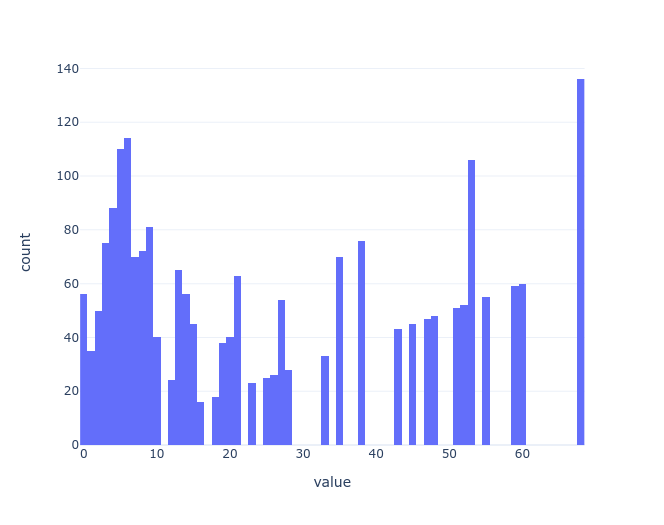
\includegraphics[width=0.5\textwidth]{figures/120_dataset/counts_histogram.png}
%     \label{fig:dataset:counts_hist}
%     }
%     \subfloat[Violin plot]{
%     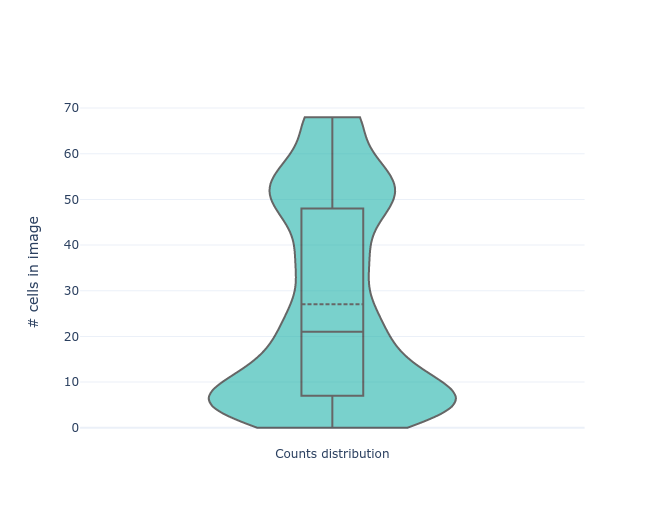
\includegraphics[width=0.5\textwidth]{figures/120_dataset/counts_violin.png}
%     \label{fig:dataset:counts_violin}
%     }
%     \caption{\textbf{Counts distribution.} Distributions of the number of annotated cells across all images in the dataset.}
%     \label{fig:dataset:counts_distrib}
% \end{figure}


\begin{figure}
    \centering
    \subfloat[Histogram]{
    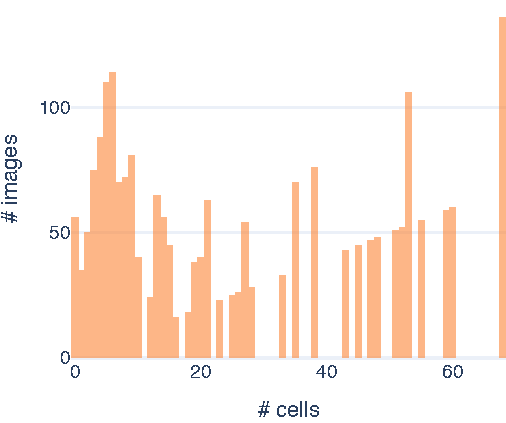
\includegraphics[width=0.6\textwidth]{figures/120_dataset/features/count_histogram.pdf}
    \label{fig:dataset:counts_hist}
    }
    \subfloat[Violin plot]{
    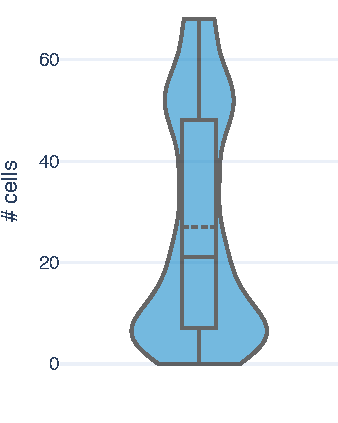
\includegraphics[width=0.4\textwidth]{figures/120_dataset/features/count_violin.pdf}
    \label{fig:dataset:counts_violin}
    }
    \caption{\textbf{Counts distribution.} Distributions of the number of annotated cells across all images in the dataset.}
    \label{fig:dataset:counts_distrib}
\end{figure}

\section{Challenges}

% Although many efforts were made to stabilize the acquisition procedure, the images present several relevant challenges for the detection task. 
% For example, the variability in brightness and contrast causes some fickleness in the pictures overall appearance (cfr. \cref{fig:dataset:dark,fig:dataset:bright}).  
% Also, the cells themselves exhibit varying saturation levels due to the natural fluctuation of the fluorescent emission properties (cfr. \cref{fig:dataset:dark,fig:artifacts:clumping}).
% Moreover, the substructures of interest have a fluid nature. This implies that the size and shape of the stained cells may change significantly (see \cref{fig:artifacts:clumping}, right), making it even harder to discriminate between them and the background. 
% Combined to that, artifacts (\cref{fig:artifacts:stripe,fig:artifacts:macaroon}), bright biological structures -- like neurons' filaments -- (\cref{fig:artifacts:stripe}) and non-marked cells similar to the stained ones handicap the recognition task. 
% Last but not least, another source of complexity is the broad shift in the number of target cells from image to image.
% Indeed, the total counts range from no stained cells (\cref{fig:dataset:empty}) to several dozens clumping together (\cref{fig:artifacts:clumping}). 
% As a consequence, this requires a model with both high precision -- to prevent false positives in the former case -- and high recall -- since considering two or more touching neurons only once produces false negatives.
% % In the former case, the model needs high precision in order to prevent false positives. The latter, instead,
% % requires high recall since considering two or more touching neurons only once produces false negatives. 

% \note[Luca][notesyellow]{Aggiungere unbalanced dataset}

Although many efforts were made to stabilize the acquisition procedure, the images present several relevant challenges for the detection task. 

Graphical properties of the pictures are undoubtedly valuable information for the classification of the pixels. However, that alone is not enough.
Indeed, an elementary approach would be to apply selection cuts over these features to separate cell pixels from the background.
Nonetheless, the characterization of cells in terms of color, saturation and contrast varies from image to image, making it difficult to generalize hard-coded thresholds.
For example, the tissues can sometimes soak in some of the marker, causing irrelevant compounds to emit light which is then captured by the microscope. 
When that is the case, the background assumes a similar hue to the neuronal cells (cfr. \cref{fig:dataset:dark,fig:dataset:bright}), and the identification falls back to other characteristics such as saturation and contrast.
In addition to that, fluorescent emissions are naturally unstable, thus generating fluctuations of the saturation levels exhibited by pixels belonging to cells (cfr. \cref{fig:dataset:dark,fig:artifacts:clumping}).

Moreover, the substructures of interest have a fluid nature. This implies that the size and shape of the stained cells may change significantly (see \cref{fig:artifacts:clumping}, right and \cref{fig:dataset:geom_area}), making it even harder to discriminate between them and the background.

Another challenge is represented by artifacts, i.e. fictitious objects accidentally present in pictures which resemble neuronal cells in terms of shape, size or color.
One example is when the marker forms accumulations of fluorophore in narrow areas that generate emissions very similar to the ones of the cells. In such cases, thresholding becomes ineffective and one has to resort to physiological characteristics as cells' shape and size in order to distinguish them from such artifacts.
Nevertheless, the distinction is not always unambiguous and this poses an issue of intrinsic subjectivity in the annotation process, which is then reflected on model performance.

A further source of complexity is represented by the broad shift in the number of target cells from image to image.
Indeed, the total counts range from no stained cells (\cref{fig:dataset:empty}) to \sidenote[Luca][notesyellow]{approfondire meglio per giustificare ablations study...magari inserendo più immagini come esempi di overcrowding}several dozens clumping together (\cref{fig:artifacts:clumping}). 
As a consequence, this requires a model with both high precision -- to prevent false positives in the former case -- and high recall -- since considering two or more touching neurons only once produces false negatives.

Last but not least, the objects are typically small and cover only marginal portions of the images. This generates an extreme imbalance between signal and background, which is even worsened by the high resolution of the pictures.
Hence, dedicated learning strategies are demanded to mitigate this issue during the training phase.

By and large, all of these factors make the recognition and counting tasks more problematic and complicate the learning process.
Likewise, borderline annotations hinder model evaluation as their subjectivity deprives the model of a reliable and indisputable testbed.
% \chapter{Methods}
\label{chap:partI_methods}

This work tackles the problem of segmenting and counting cells in a \textit{supervised learning} framework. For this purpose, we address the segmentation task exploiting four CNN architectures belonging to the Unet and ResUnet families. 
Once the cells are detected, the final count is retrieved as the number of connected pixels in the post-processed output.
In doing so, we also test the impact of study design choices intended to reduce false negatives and promote accurate segmentation.
In addition to that, the four architectures are compared to an adaptive thresholding approach used as a baseline. 

\section{Non-ML baseline}
\label{baseline}

Machine Learning and Deep Learning have succeeded in many applications from several domains lately, thus building great expectations and becoming hot topics in current innovation processes at various societal levels.
Nevertheless, these powerful techniques are not a magic bullet to solve any data-related problem \cite{wolpert1997nofreelunch}. They come with their own challenges and limitations that are often overlooked in real-world applications, possibly causing thunderous failures due to unjustified expectations.
In fact, it is not unusual to fall victim to their popularity only to find months down the line that more straightforward methods work best for some specific task or data.

To avoid incurring in this ``ML hype curse", this work considers a simple non-ML approach as a baseline. 
In particular, an adaptive thresholding mechanism is implemented to exploit the pixel intensity information for binarization.
In practice, the input image is read as grayscale and a selection cutoff is set as a configurable quantile of the pixel intensity distribution.
A binary mask is obtained by labeling pixels above that threshold as cells, and the rest as background.
After that, the same post-processing steps as the ones adopted for the output of the ML models are applied (see \cref{sec:post_processing}).
This operation is performed for all training and validation pictures, and the goodness of fit is assessed as described in \cref{sec:model_evaluation}.
The whole procedure is then repeated varying the quantile value used for thresholding. A starting search is conducted using a coarse grid from 0.9 to 0.99 with steps of 0.01. This is intended to explore the hyperparameter space and get an idea of where the approach performs best. 
Since this happens for higher values, a finer grid from 0.97 to 0.999 with steps of 0.001 is exploited for fine-tuning.
Finally, the cutoff corresponding to the highest $F_1$ score is chosen as the optimal threshold and is later used to assess the baseline performance on the test set.

\section{Model architecture}
\label{model_architecture}

\begin{figure}
\centerline{
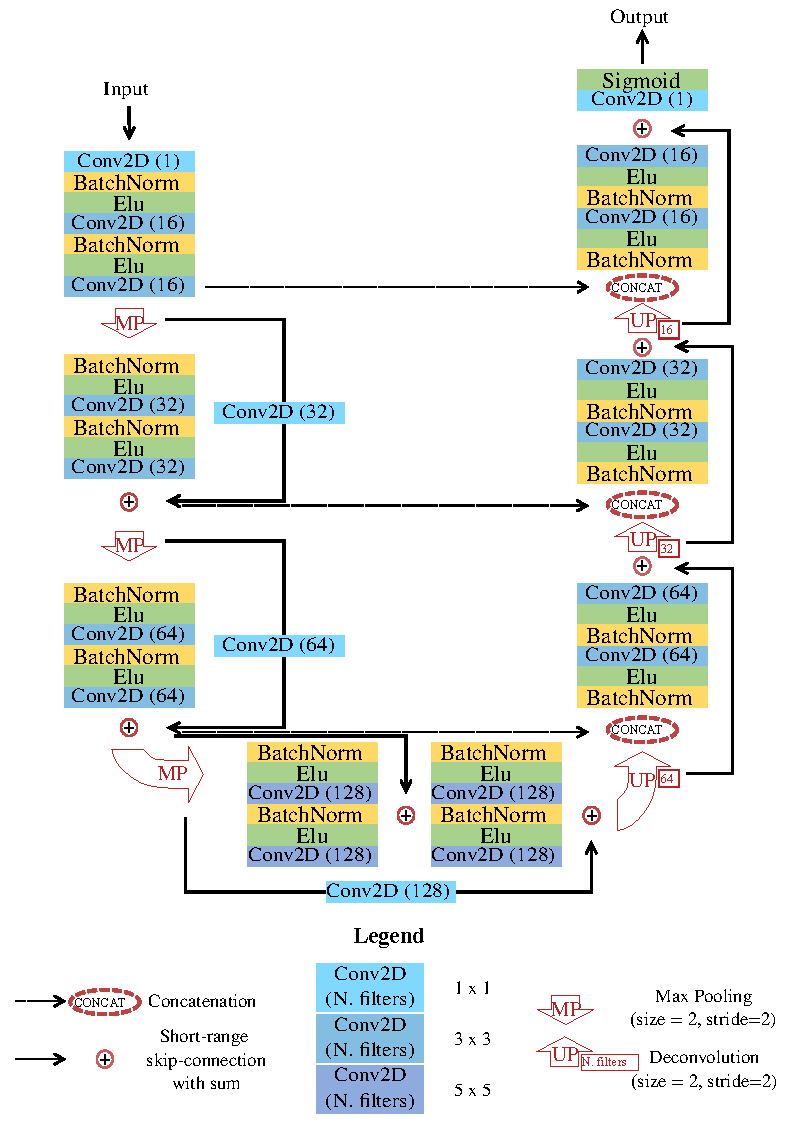
\includegraphics[width=0.8\textwidth]{figures/130_methods/c-resunet_architecture.pdf}
}
\caption{\textbf{Model architecture}. Each box reports an element of the entire architecture (individual descriptions in the legend). 
% The shortcut-connections along the encoding-path are supported by a 1$\times$1 convolution to enable the final sum before the max-pooling operation.
} \label{fig:model_architecture}
\end{figure}
We compare the detection and counting performance of four alternative architectures derived from two network families -- Unet and ResUnet -- commonly used for segmentation tasks.
In the former family, we pick the original Unet architecture \cite{unet} and a smaller version (small Unet) obtained by setting the initial number of filters equal to the ResUnet proposed in \citeA{deep_resunet} and scaling the following blocks consequently.
In the latter, we pick a ResUnet implementation presented in \citeA{deep_resunet} and a similar version with minor modifications.
Specifically, we add an initial 1$\times$1 convolution to simulate an RGB to grayscale conversion.
The advantage of doing so -- as opposed to apply a standard grayscale conversion -- is that the transformation is learned during training so to improve the segmentation performance.
As a further modification, we insert an additional residual block having 5$\times$5 filters -- instead of 3$\times$3 -- at the end of the encoding path. This adjustment should provide the model with a larger field of view, thus fostering a better comprehension of the context surrounding the pixel to classify.
This kind of information can be beneficial, for example, when cells clump together and pixels on their boundaries have to be segmented. 
Likewise, the analysis of some background structures (\cref{fig:dataset:bright,fig:artifacts:stripe,fig:artifacts:macaroon}) can be improved by looking at a broader context.
The resulting architecture is reported in \cref{fig:model_architecture} and it will be referred to as \textbf{cell ResUnet (c-ResUnet)} hereafter.

\section{Ablation studies}
\label{sec:ablation_studies}

Alongside the comparison of different approaches, we also tested the effect of two design choices intended to mitigate errors on challenging images containing artifacts and cells overcrowding.

% \noindent\textbf{Artifacts Oversampling (AO)}.
\subsection{Artifacts Oversampling (AO)}

The presence of biological structures or artifacts like those in \cref{fig:artifacts:macaroon,fig:artifacts:stripe}  can often fool the model into detecting false positives. 
% Indeed, their similarity with cells in terms of saturation and brightness makes it difficult for the model to handle them correctly. 
Indeed, their similarity with cells in terms of saturation and brightness hampers their correct handling.% by the model.
In addition, only a handful of examples of such structures are available, making them underrepresented in the data and complicating the task even further.
For this reason, we tried to increase the augmentation factor for these inputs to facilitate the learning process. Specifically, we selected 6 different crops representing such relevant structures and re-sampled them with the augmentation pipeline described in \cref{sec:model_training}, resulting in 150 new images for each crop.

\note[Luca][notesyellow]{riportare crop artefatti?}
% The transformations applied regarded rotations, addition of gaussian noise, elastic transformation and brightness, hue, saturation variation.

% \noindent\textbf{Weight Maps (WM)}. 
\subsection{Weight Maps (WM)} \label{sec:weights_map}

One of the toughest challenges during the inference is related to cell overcrowding. 
As a matter of fact, failing to precisely segment cells boundaries may lead to spurious connections between objects that are separated. Consequently, multiple objects are considered as a single one and the model performance deteriorates.
In order to improve cell separation, \citeA{unet} suggested leveraging a weight map that penalizes more the errors on the borders of touching cells.
Building on that, we introduce a novel implementation where single object contributions are compounded additively.
This procedure generates weights that decrease as we move away from the borders of each cell. 
At the same time, the contributions coming from single items are combined so that the global weight map presents higher values where more cells are close together (see \cref{fig:weight_calculation}).
%
% \begin{figure}
% \centerline{
%      \begin{subfigure}[]{0.4\textwidth}
%          \centering
%          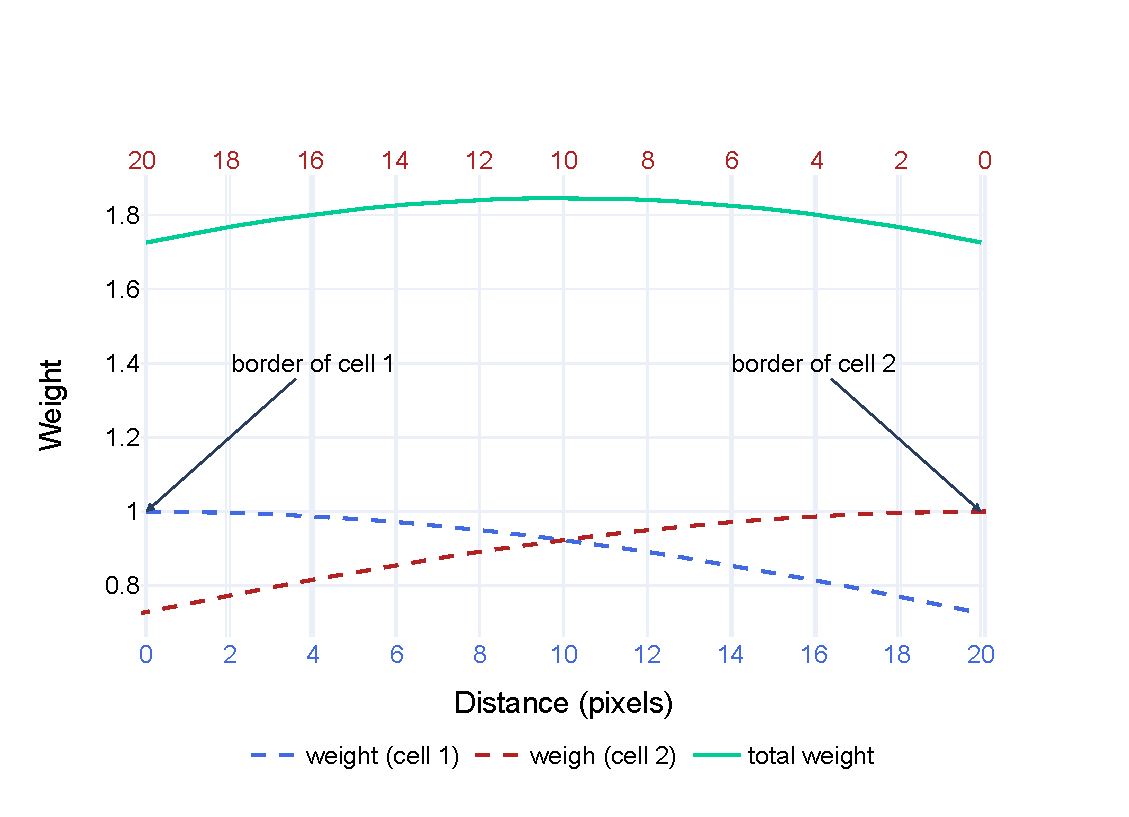
\includegraphics[width=\textwidth]{figures/130_methods/weight_calculation.eps}
%         \caption{Weight compounding}
%         \label{fig:weight_calculation}
%      \end{subfigure}
%      \begin{subfigure}[]{0.62\textwidth}
%          \centering
%          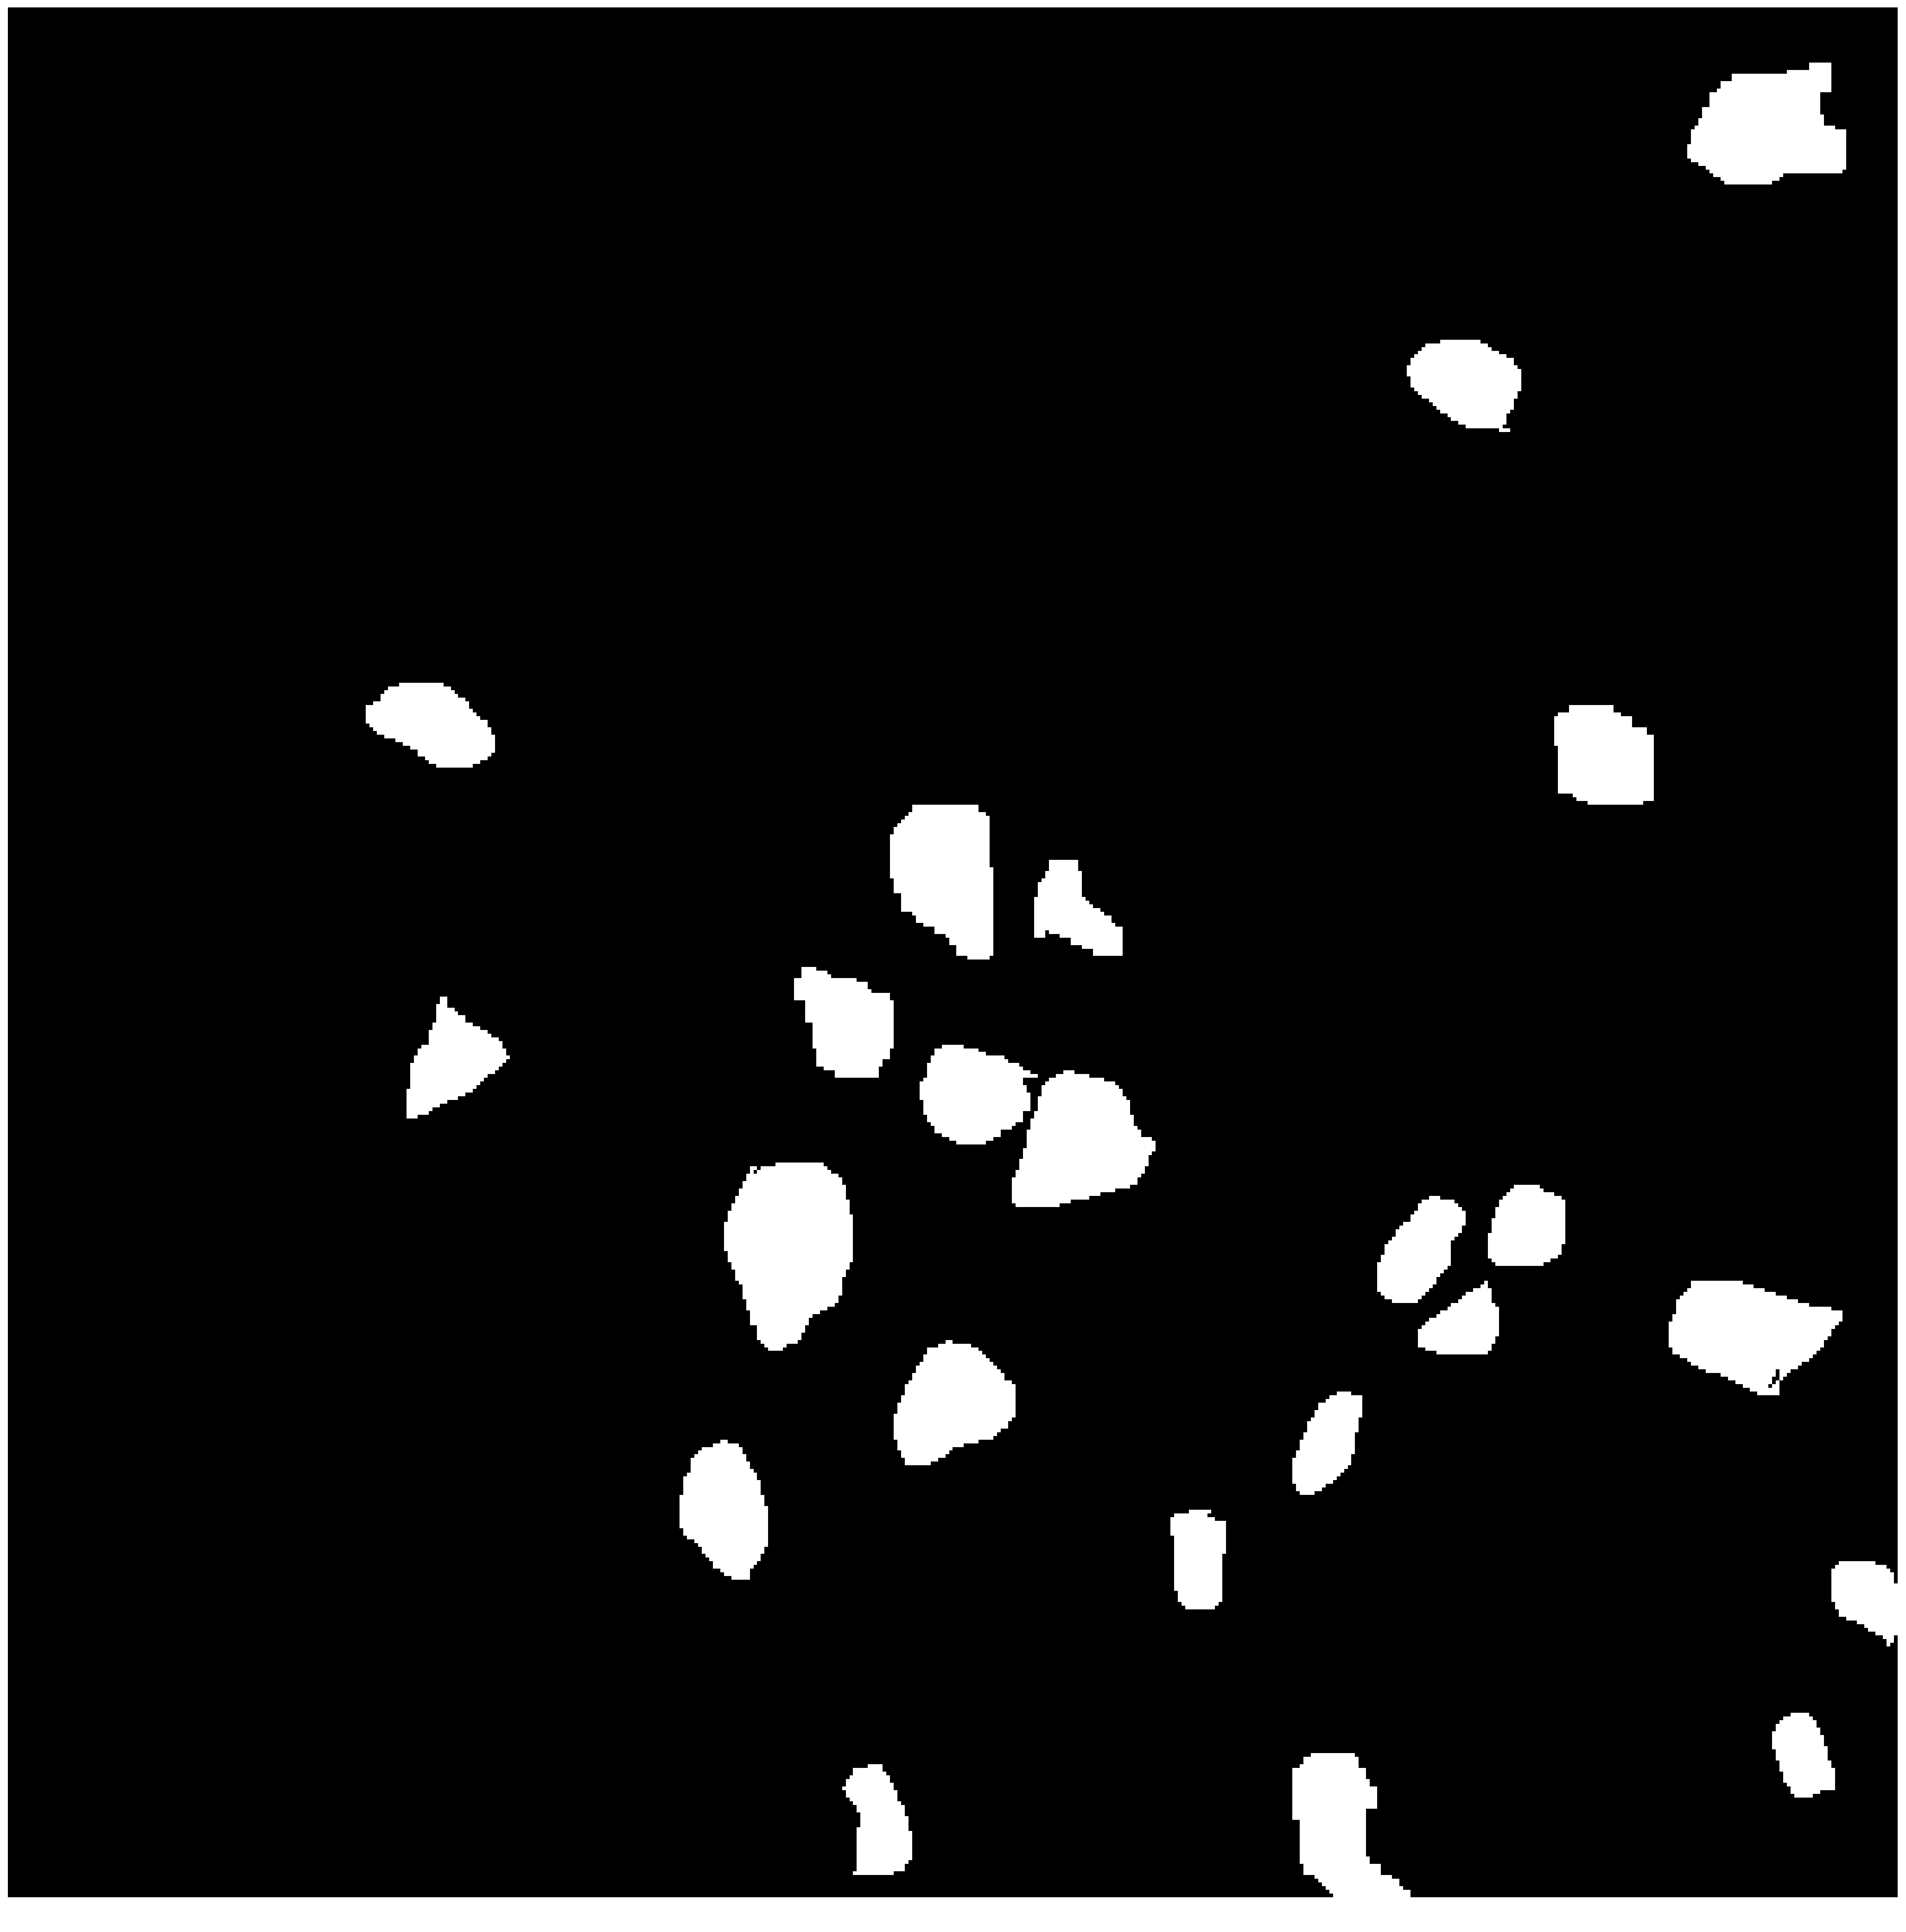
\includegraphics[ width=0.45\textwidth]{figures/130_methods/crop_mask_2451_crop.jpeg}
% 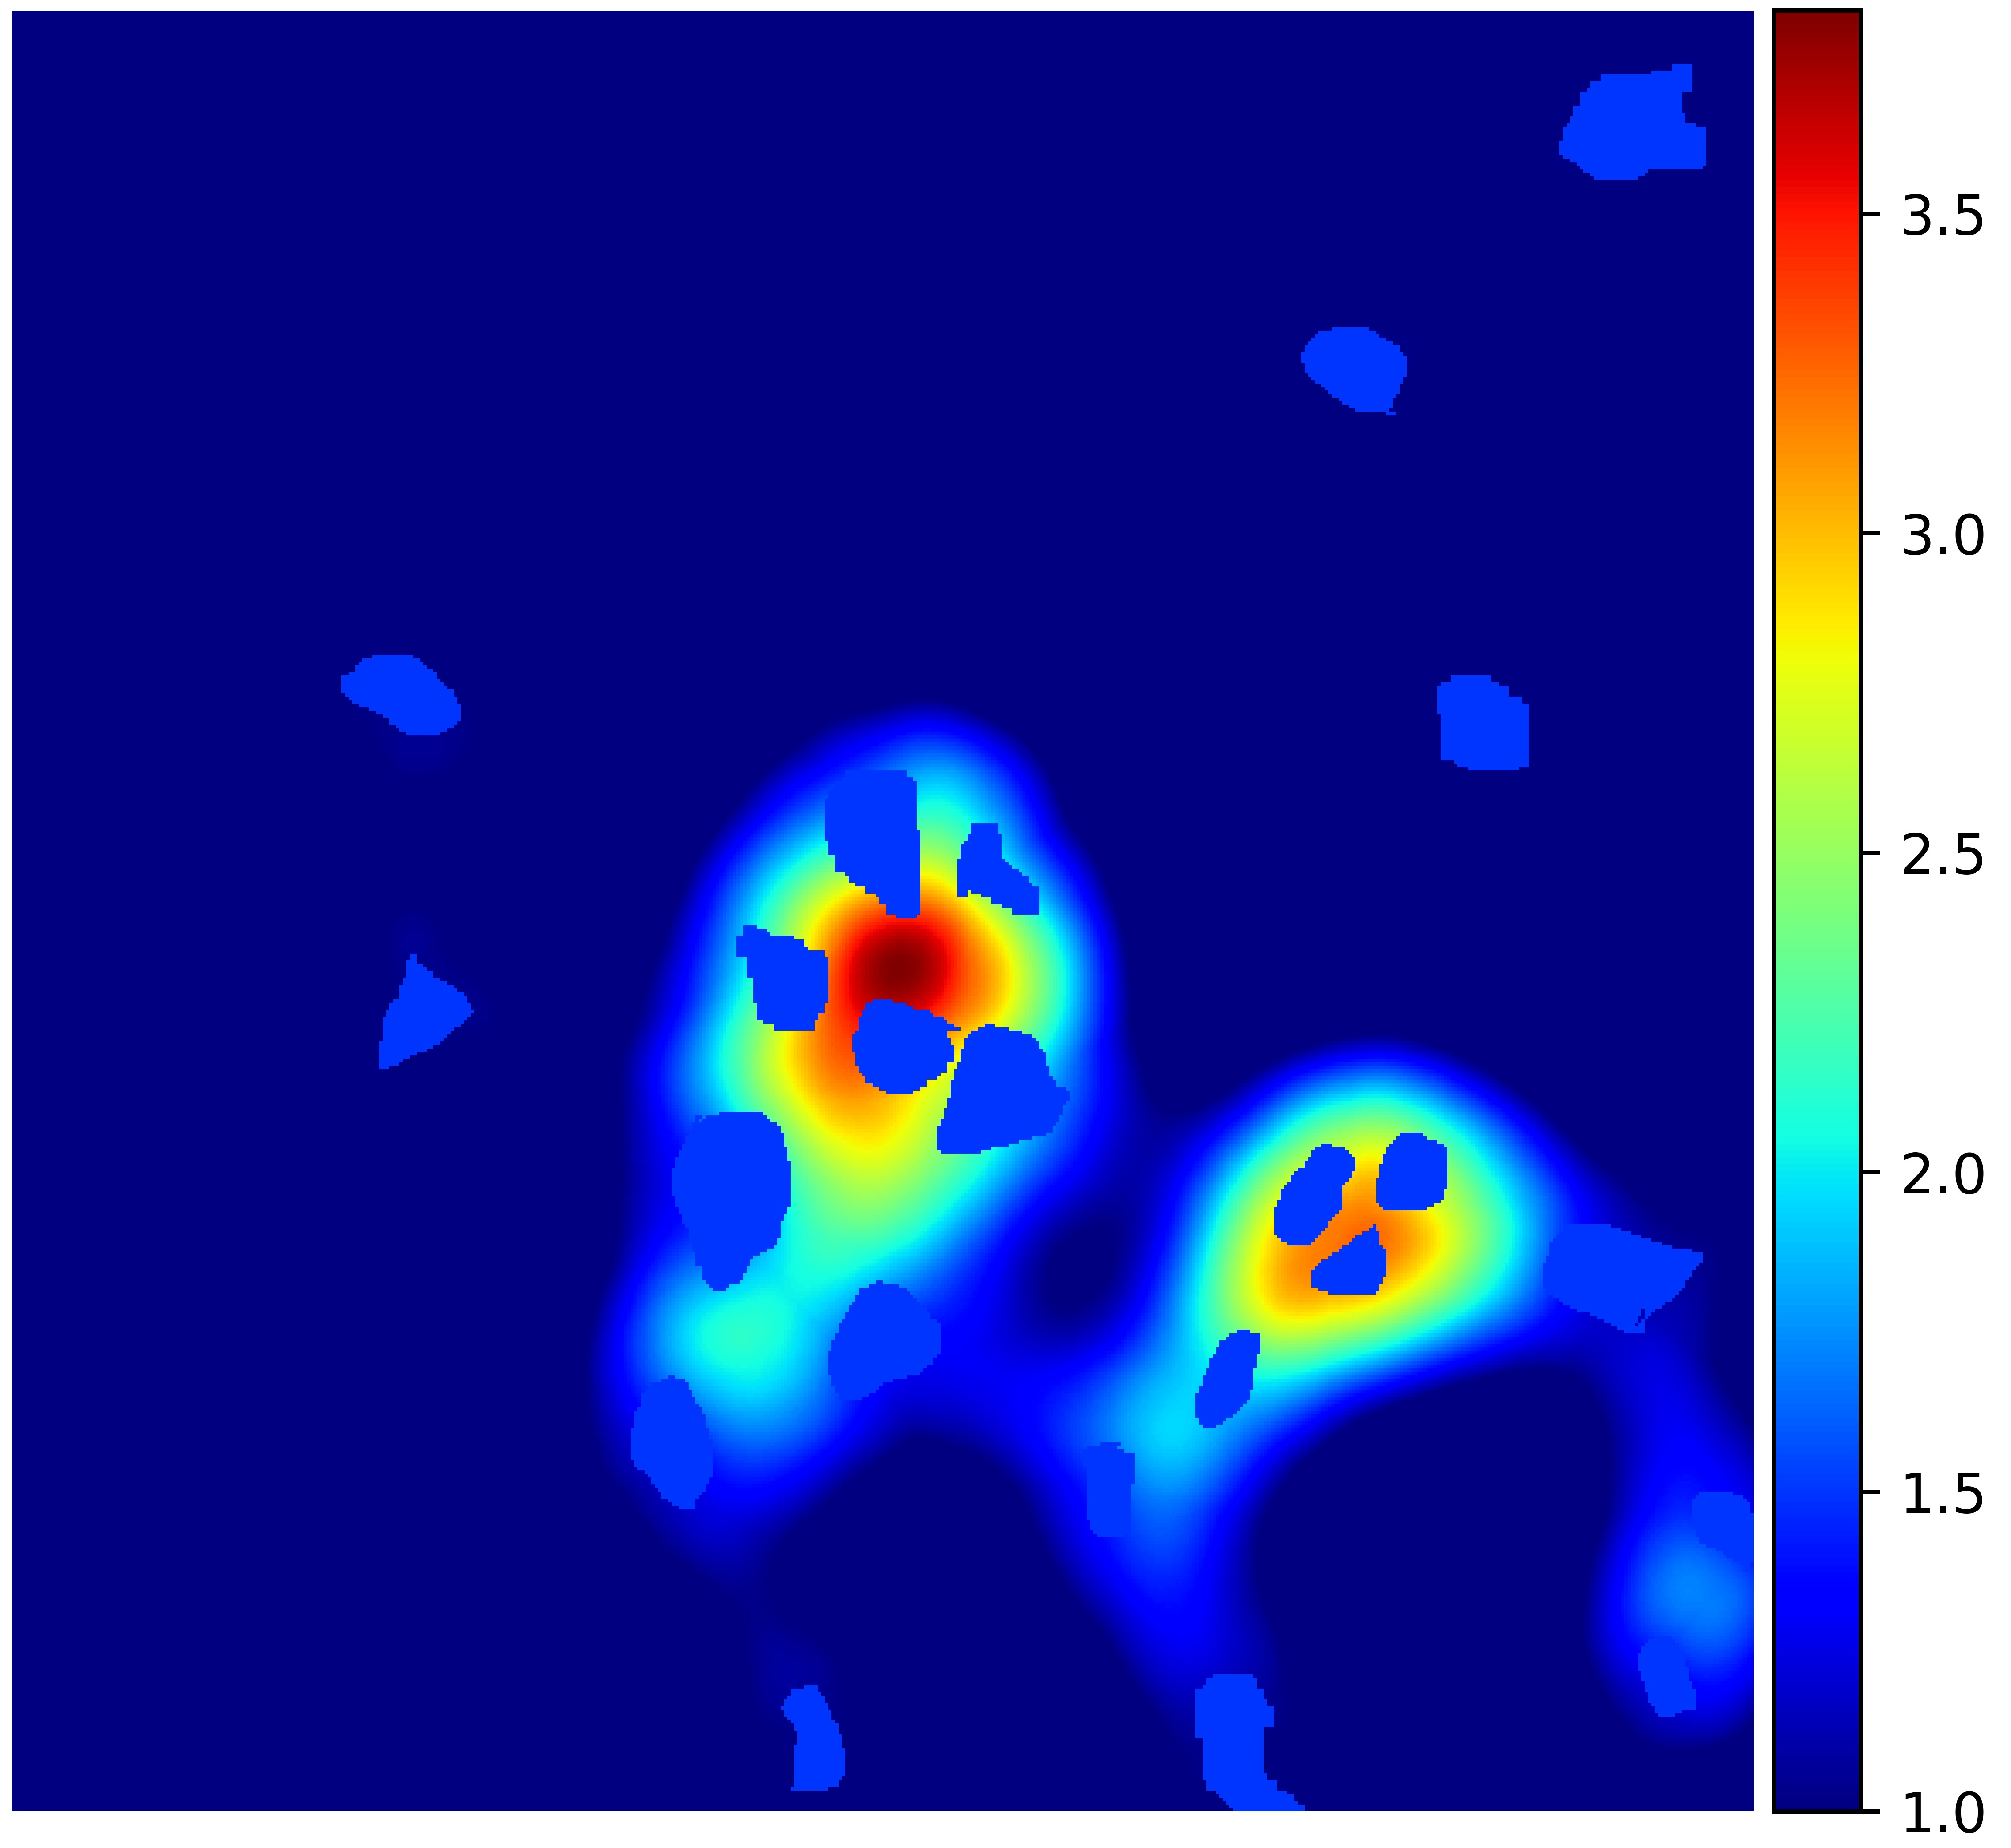
\includegraphics[trim=0 0.008in 0 0, width=0.50\textwidth]{figures/130_methods/crop_weigths_2451_crop.jpeg}
%          \caption{Mask and correspondent weight map}
%          \label{fig:weight_map_example}
%      \end{subfigure}
% }
% \caption{\textbf{Weight map}. 
% \ref{fig:weight_calculation} shows the weight factors of background pixels between cells according to Eq. (\ref{weight_formula}). The dashed curves depict the weights generated by single cells as a function of the distance from their borders.
% % , respectively cell 1 on the left (blue) and cell 2 on the right (red).
% The green line illustrates the final weight obtained by adding individual contributions. 
% In \ref{fig:weight_map_example}, a target mask and the corresponding weight map.} 
% \label{fig:weight_map}
% \end{figure}
%
\begin{figure}
    \centering
    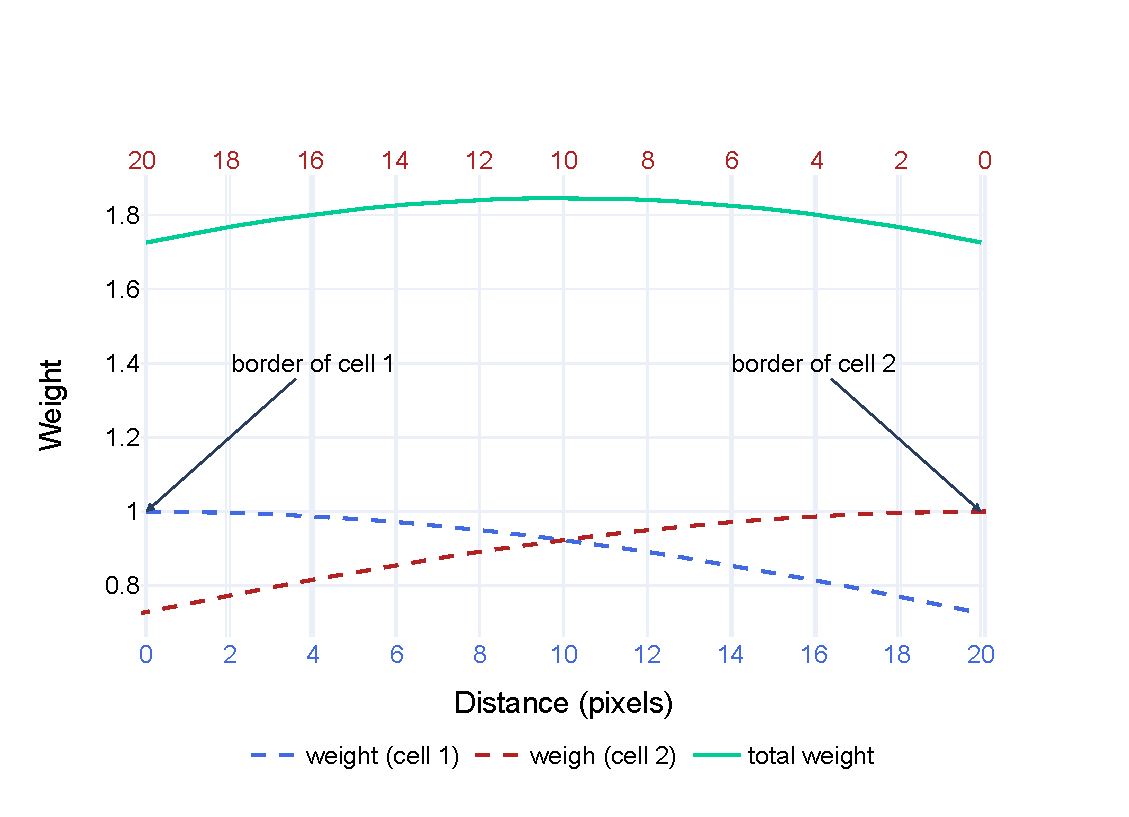
\includegraphics[width=.6\textwidth]{figures/130_methods/weight_calculation.eps}
    \caption{\textbf{Weight compounding.}
    The dashed curves depict the weights generated by single cells as a function of the distance from their borders according to \cref{eq:weight_formula}.
    The green line illustrates the final weight obtained by adding individual contributions.}
    \label{fig:weight_calculation}
\end{figure}
%
\begin{figure}
    \centering
    \subfloat[Mask]{
    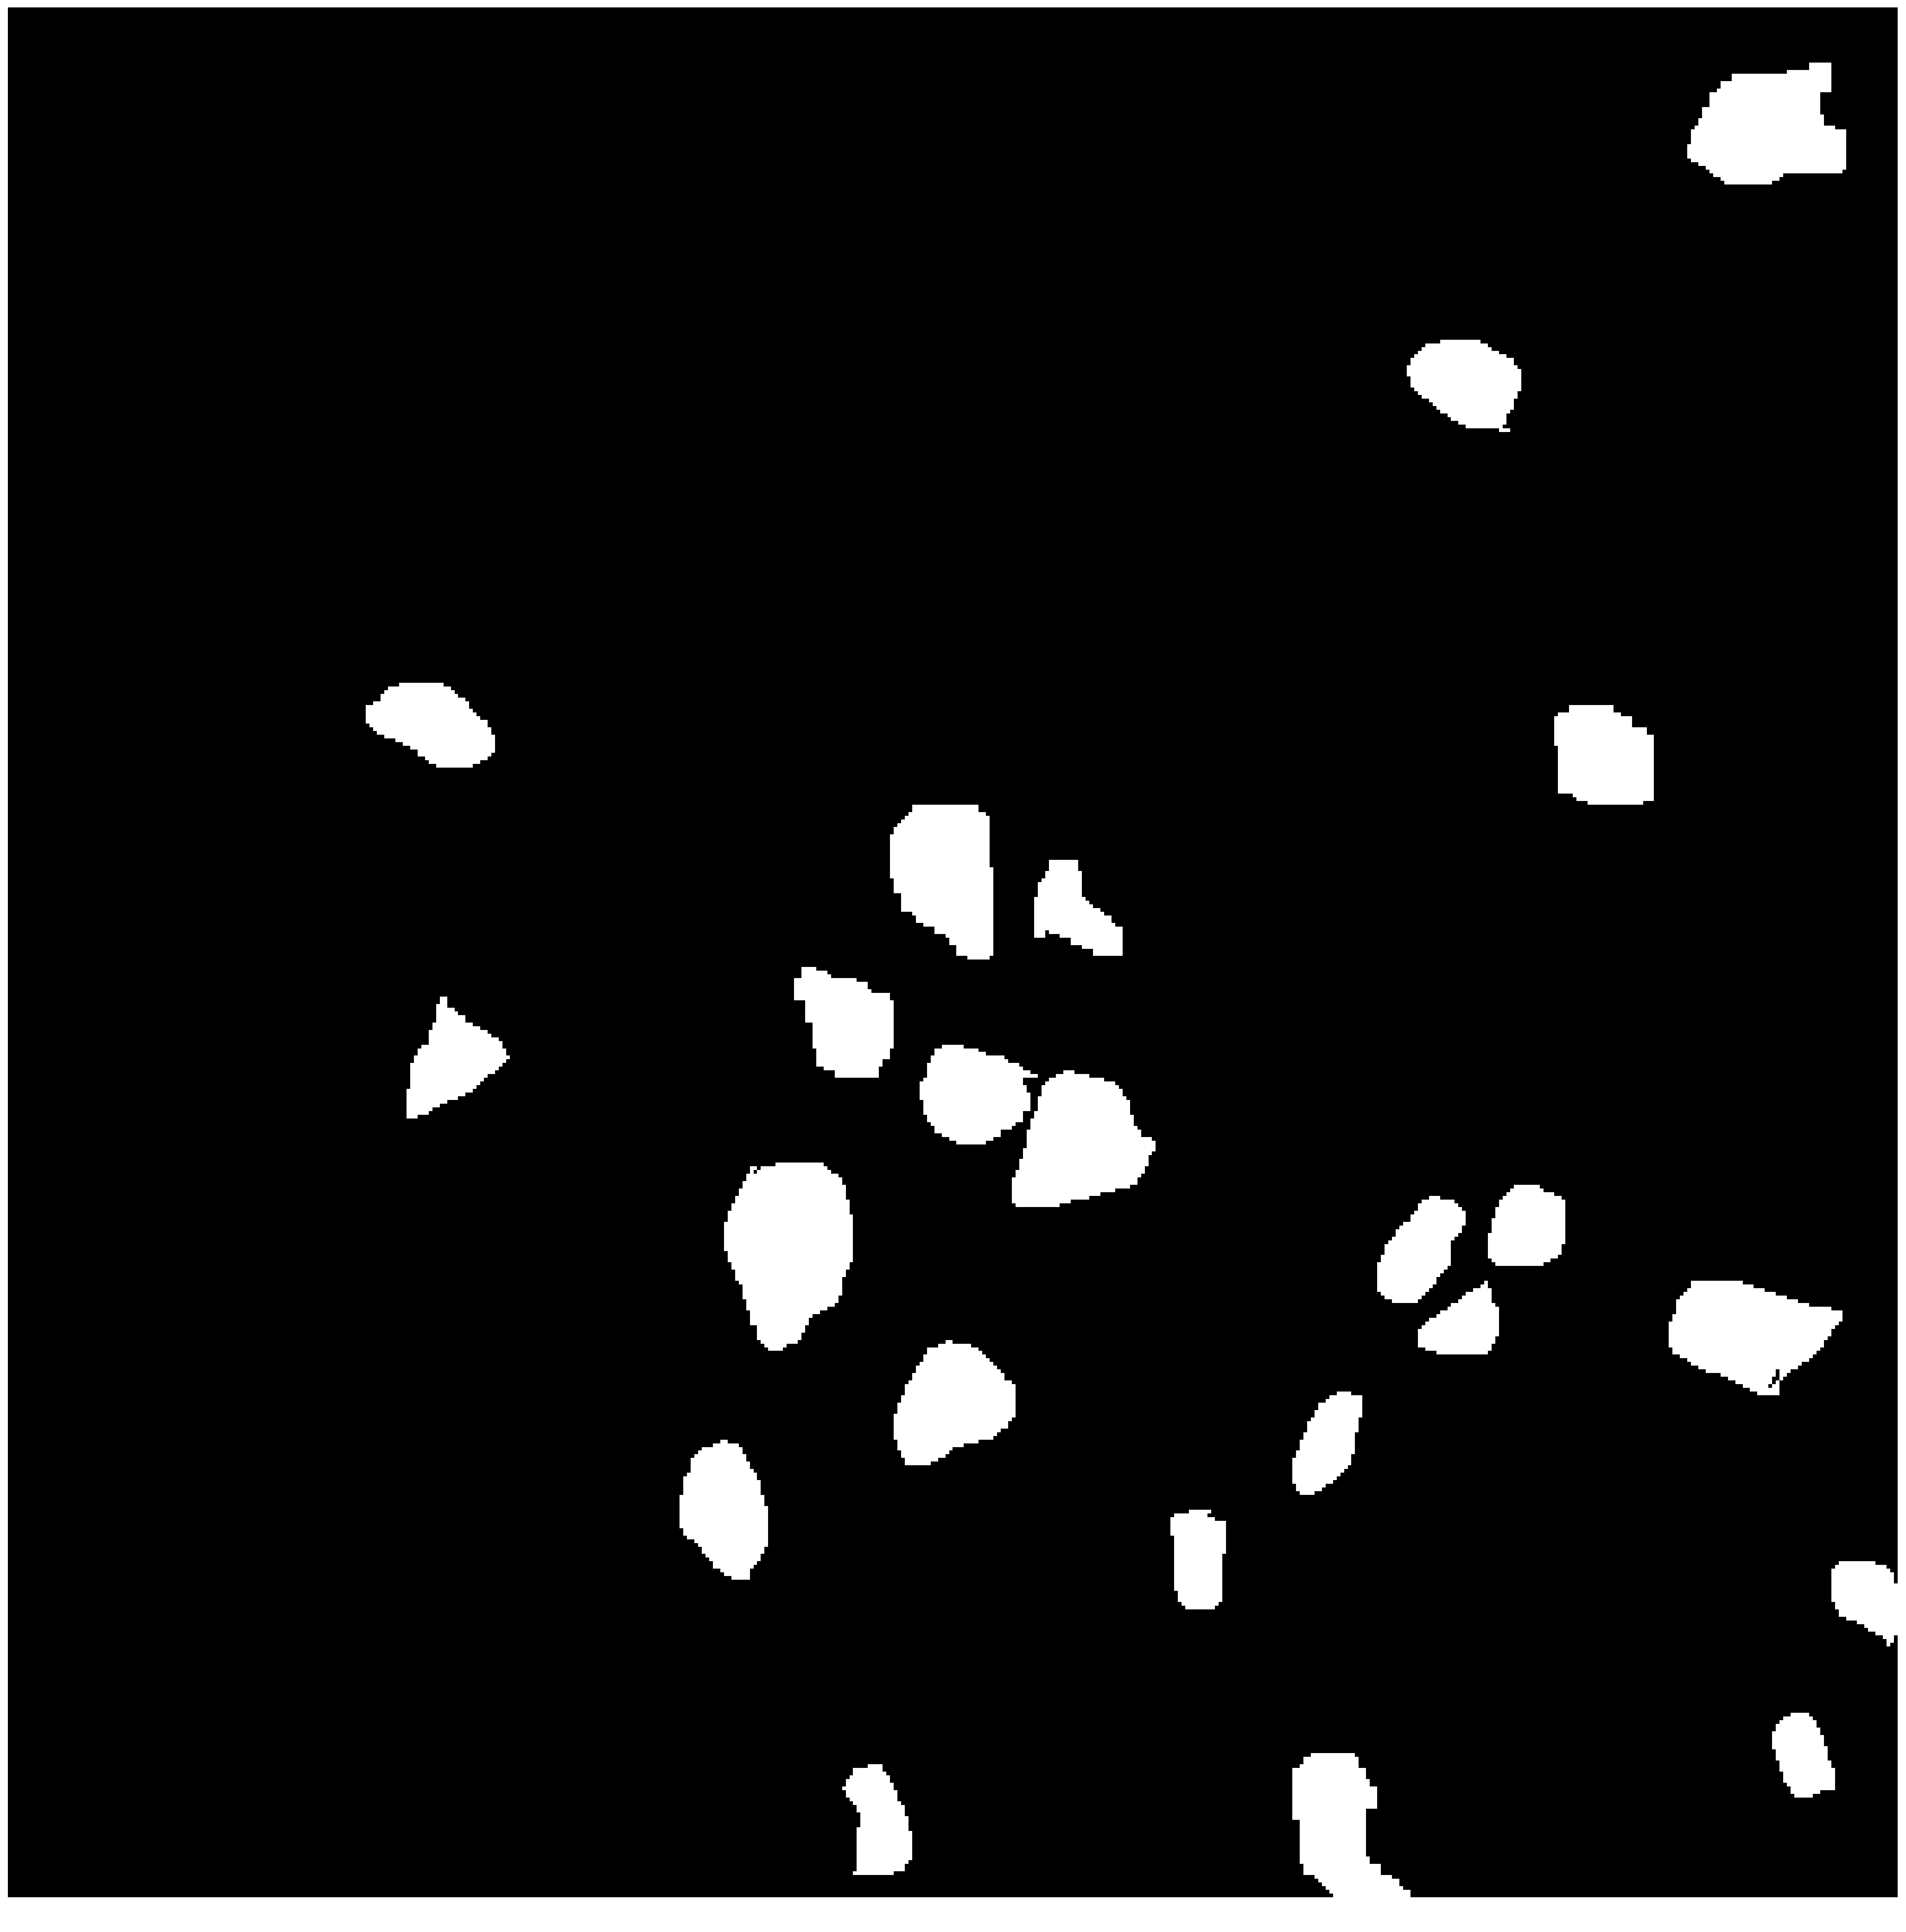
\includegraphics[width=0.45\textwidth]{figures/130_methods/crop_mask_2451_crop.jpeg}
    }
    \subfloat[Weight map]{
    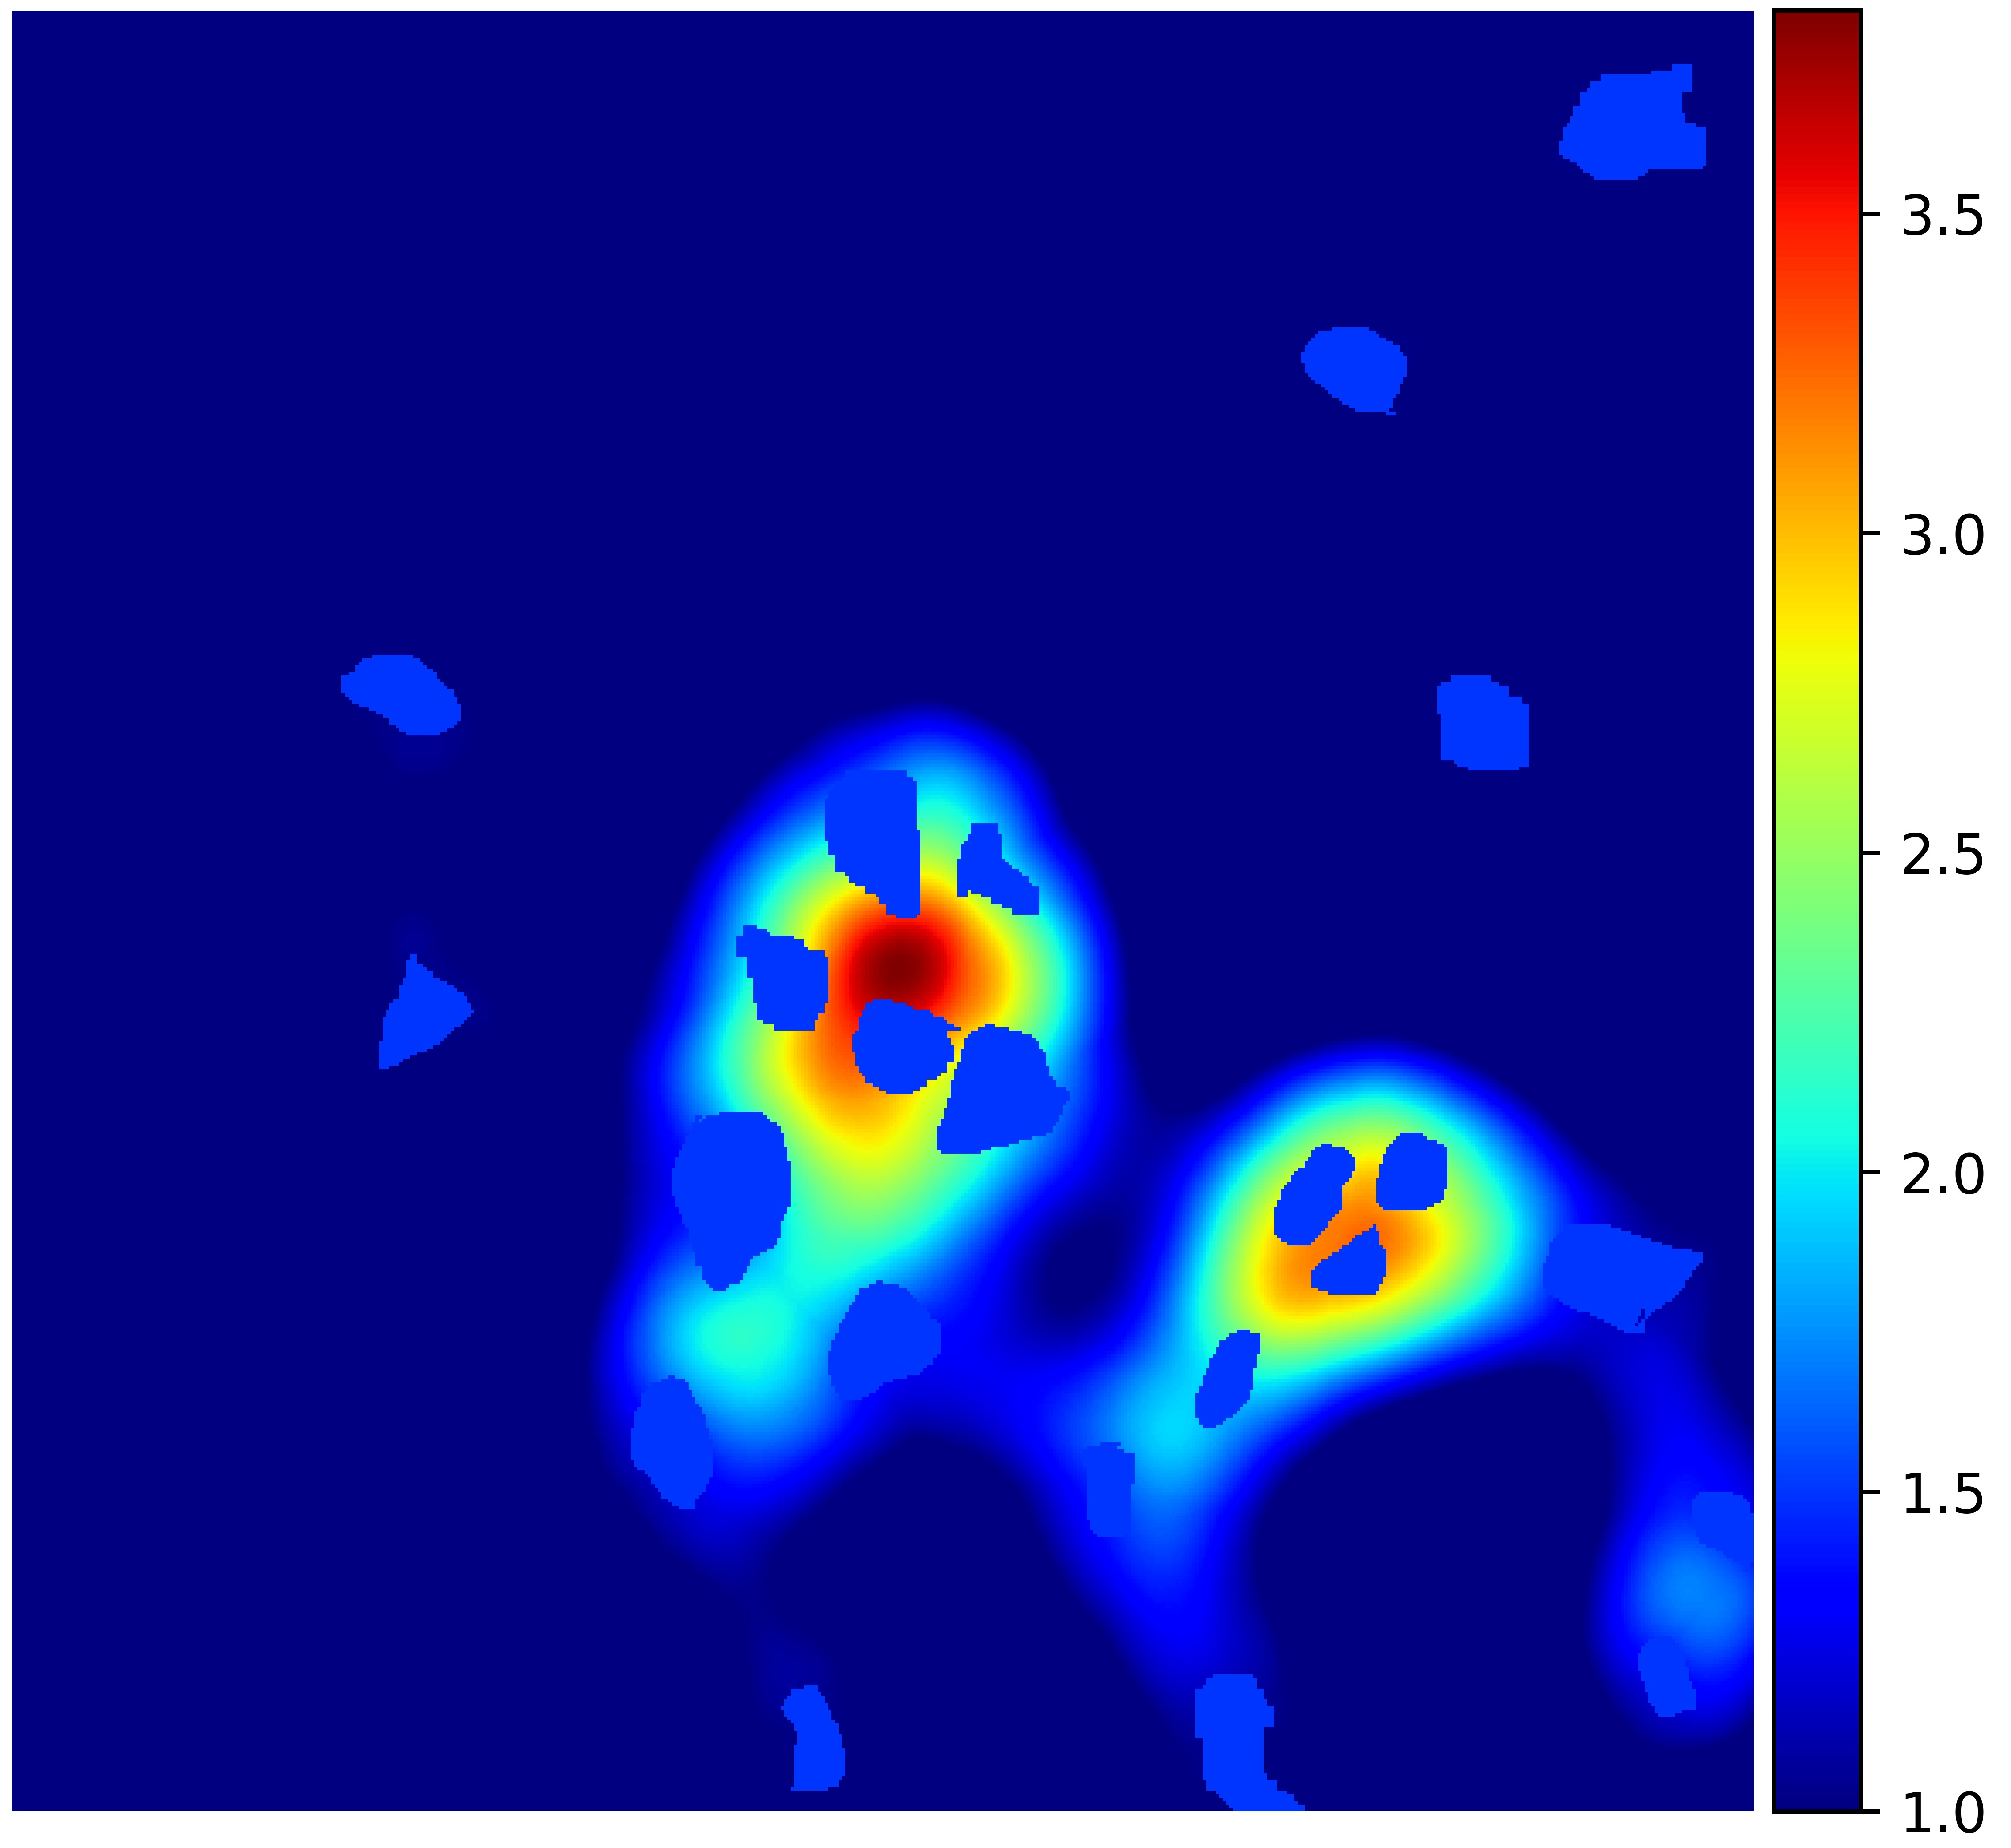
\includegraphics[trim=0 0.008in 0 0,
    width=0.50\textwidth]{figures/130_methods/crop_weights_2451_crop.jpeg}
    }
    \caption{\textbf{Weight map.} A target mask and the corresponding weight map}
    \label{fig:weight_map_example}
\end{figure}
%
The pseudocode\footnote{full implementation \githubweights} for a weight map is reported in Alg. \ref{algo:pseudocode_weightmap}, and an example weight map is shown in \cref{fig:weight_map_example}.

\begin{algorithm}%[H]
% \begin{algorithmic}[1]
\DontPrintSemicolon
     Initialize empty $\text{map}_j$ (mask size)\tcp*{weight map $j$-th mask}
    \For{each cell in mask} 
    {
    \tcc{loop over $i$-th cell in $j$-th mask}
         Initialize empty $\text{map}_i$  (mask size) \tcp*{weight map $i$-th cell}
        
         Add $i$-th cell to $\text{map}_i$
        
         Compute euclidean distance between each pixel of $\text{map}_i$ and the closest pixel of the $i$-th cell \label{step:distance}
        
         Compute each pixel's weight in $\text{map}_i$ according to a decreasing exponential function:
        \begin{equation}
        % \hskip 4.5cm
        \text{weight} = \exp\left\{\dfrac{-d^{2}}{2\sigma^{2}}\right\}
        \label{eq:weight_formula}
        \end{equation}
        
        \tcc {$d$ is the distance computed at step \ref{step:distance}}
        \tcc {$\sigma$ is a customizable parameter set to 25 (average cell radius)}
        
    Sum the resulting $\text{map}_i$ to the full $\text{map}_j$
    % , as illustrated in Fig. \ref{fig:weight_calculation};
}
% \end{algorithmic}
\caption{weight map pseudocode for $j$-th mask}
\label{algo:pseudocode_weightmap}
\end{algorithm}

\section{Model training}
\label{sec:model_training}
After randomly setting 70 full-size images apart as a test set, the remaining pictures were randomly split into training and validation sets. 
In particular, twelve 512x512 partially overlapping crops were extracted from each image and fed as input to the network after undergoing a standard augmentation pipeline. Common transformations were considered as rotations, addition of Gaussian noise, brightness variation and elastic transformations \cite{elastic_tranformation}. 
The crops augmentation factors were fixed differentially based on their contents. 
The 6 crops included in the artifact oversampling ablation study were re-sampled 25 times each.
Instead, all the remaining crops produced 10 augmented versions for manually segmented images and 4 for all the others.
As a result, the model was trained on a total of nearly 16000 images (70\% for training and 30\% for validation).

All competing architectures were trained from scratch under the same conditions to favour a fair comparison.
Specifically, the Adam \cite{adam} optimizer was employed with an initial learning rate of 0.006. A a scheduled decrease of 30\% was then applied if the validation loss did not improve for four consecutive epochs. 
A \textbf{weighted binary cross-entropy} loss was adopted on top of the weight maps to handle the imbalance of the two classes (weights equal to 1.5 and 1 for cells and background, respectively).
All models were trained until no improvement was observed for 20 consecutive epochs. In this way, each model was allowed to converge and the comparison was made at the best of each architecture's individual capabilities.

The approach was implemented through Keras API \cite{keras} using \texttt{TensorFlow} \cite{tensorflow} as backend. For more details, please refer to the GitHub repository\footnote{\github}.
The training was performed on 4 V100 GPUs provided by the \textit{Centro Nazionale Analisi Fotogrammi} (CNAF)\footnote{\cnaf} computing center of the \textit{National Institute for Nuclear Physics}\footnote{\infn} in Bologna.


\section{Post-processing} \label{sec:post_processing}

\begin{figure}
    \begin{subfigure}{\textwidth}
        \centering
        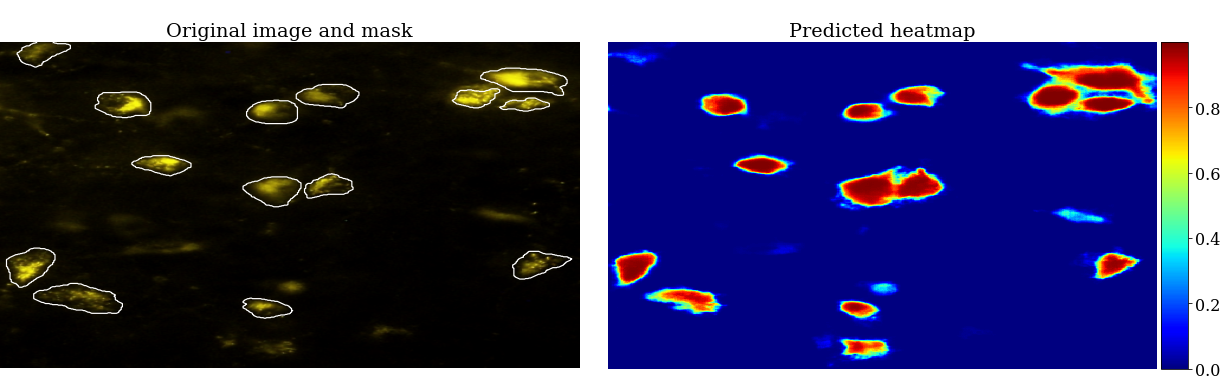
\includegraphics[width=\textwidth]{figures/130_methods/orig+heatmap:278.png}
        \caption{
        % Original image and raw output
        }
        \label{fig:raw_output}
        \end{subfigure}
    \begin{subfigure}{\textwidth}
        \centering
        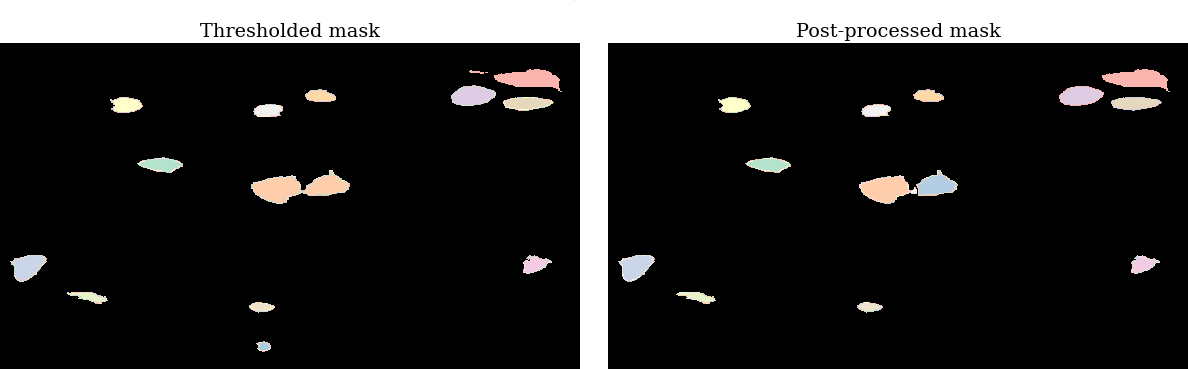
\includegraphics[width=\textwidth]{figures/130_methods/thresh+post_proc:278.png}
        \caption{
        % Thresholded and post-processed predicted masks
        }
        \label{fig:thresh+post_proc}
        \end{subfigure}
    \caption{\textbf{Model output}. 
    Top: the input image with white contours indicating annotated cells  (left) and the model's raw output  (right).
    Bottom: the predicted mask after thresholding at 0.875 (left) and the predicted mask after post-processing (right).}
    \label{fig:model_output}
\end{figure}
The final output of the model is a probability map (or heatmap), in which each pixel value represents the probability of belonging to a cell. 
% An example of this outcome is reported on the right of the \ref{fig:raw_output} if the input image on the left is provided to the model.
\Cref{fig:raw_output} reports an example of an input image (left) and the corresponding predicted heatmap (right).
% An example of this outcome is reported in the Fig. \ref{fig:raw_output} (right) if a sample input image (left) is provided to the model.
The higher the value, the higher is the confidence in classifying that pixel as signal. 
A thresholding operation was then applied on the heatmap to obtain a binary mask where groups of white connected pixels represent the detected cells. \Cref{fig:thresh+post_proc} (left) illustrates the cells detected after the binarization with different colors.
After that, ad-hoc post-processing was applied to remove isolated components of few pixels and fill the holes inside the detected cells. 
Finally, the watershed algorithm \cite{watershed} was employed with parameters set based on the average cell size.
\sidenote[Luca][notesyellow]{Descrivere meglio aggiungendo riferimenti nell'immagine}
An example of the results if provided in \cref{fig:thresh+post_proc}, where the overlapping cells in the middle present in the binary mask (left) are correctly splitted after post-processing (right). Also, the small object in the top right corner is removed
% , and the hole in the bottom right object is filled
.


\section{Model evaluation} \label{sec:model_evaluation}

% The Unet, small Unet, ResUnet and c-ResUnet architectures were evaluated and compared based on both detection and counting performance. 
All the presented approaches were evaluated and compared based on both detection and counting performance. 
Also, ablation studies were conducted to assess the impact of artifacts oversampling and weight maps.
% Also, ablation studies assessed the impact of artifacts oversampling and weight maps.

In order to evaluate the detection ability of the models, a dedicated algorithm was developed.
% Specifically, each target cell was compared to all objects in the corresponding predicted mask and uniquely associated with the closest one.
Specifically, each predicted object was compared to all cells in the corresponding ground-truth label and uniquely associated with the closest one.
If the distance between their centroids was less than a fixed threshold (50 pixels, i.e. average cell diameter), the predicted element was considered a match and it increased the true positive count (TP).
% ; a false negative otherwise (FN).
At the end of this procedure, all true objects without matches were considered as false negatives (FN). Likewise, the remaining detected items not associated with any target were considered as false positives (FP).
Algorithm \ref{algo:pseudocode_metrics} reports the pseudocode of the procedure described above\footnote{full implementation \githubmetrics}.
\begin{algorithm}%[H]
% \begin{algorithmic}[1]
    \DontPrintSemicolon
    % init
    \KwIn{ pred$_i$, mask$_i$}
    \KwOut {TP, FP, FN}       
    % \tcp*{true positives, false positives, false negatives}
    
    Set TP, FP, FN = 0
    
    Get predicted objects, pred\_objs$^i$
    \tcp*{detected cells}
    
    Get true objects, true\_objs$^i$
    \tcp*{annotated cells}
    
    % centers
    Get predicted centers, pred\_ctrs$^i$
    %  \tcp*{centers of predicted objects}
    
    Get true centers, true\_ctrs$^i$
    %  \tcp*{centers of true objects}
    
    \For{each ctr$_j$ in pred\_ctrs$^i$} 
        {
        \tcc{loop over predicted centers}
        \For{each ctr$_k$ in true\_ctrs$^i$}
            {
            \tcc{loop over true centers}
            
             Compute euclidean distance between ctr$_j$ and ctr$_k$ \label{step:ctrs_distance}
             
             Store distance and indexes
             \label{step:store_distance}
            } 
        
         Compute the minimum, min\_dist$_i$ of the distances stored in step \ref{step:store_distance}
         
        \If{understand}{
            Increase true positives, TP
            
            Remove ctr$_j$ from pred\_ctrs$^i$
            
            Remove ctr$_k$ from true\_ctrs$^i$
        }
        
        }
        
    Compute false negatives as true\_objs$^i$ - TP
    
    Compute false positives as pred\_objs$^i$ - TP
    
\caption{metrics computation for i\emph{-th} image}
\label{algo:pseudocode_metrics}
\end{algorithm}
Starting from these values, we referred to accuracy, precision, recall and $F_1$ score as indicators of detection performance.
% In terms of detection performance, the $F_1$ score was adopted as the primary indicator. Accuracy, precision and recall were also inspected to have a better understanding of the model ability. 
The definitions of such metrics are reported below:

\begin{align}
% \hskip 2cm
\text{accuracy} &=  \frac{\text{TP}}{\text{TP} + \text{FP} + \text{FN}}
= \frac{\text{1}}{\text{1} + \frac{1}{\text{TP}} \left(\text{FP} + \text{FN}\right)}
\label{eq:accuracy}; \\ 
\text{precision} &=    \frac{\text{TP}}{\text{TP} + \text{FP}}; \\
\text{recall} &=    \frac{\text{TP}}{\text{TP} + \text{FN}}; \\ 
F_1 \text{score} &=  \frac{2 * \text{precision} * \text{recall}}{\text{precision} + \text{recall}}
= \frac{2*\text{TP}}{2*\text{TP} + \text{FP} + \text{FN}} 
= \frac{\text{1}}{\text{1} + \frac{1}{\text{2TP}} \left(\text{FP} + \text{FN}\right)}
\label{eq:F1}.
\end{align}
% where TP, FP and FN indicates true positive (cells correctly detected), false positives (cells erroneously detected) and false negatives (cells erroneously missed), respectively. 
Notice that we do not have true negatives in \cref{eq:accuracy} since the prediction of the class ``not cell" is done at the pixel level and not at the object level, so there are no ``non-cell" objects predicted by the model.

Regarding the counting task, the Mean Absolute Error (MAE), Median Absolute Error (MedAE) and Mean Percentage Error (MPE) were used instead. More precisely, let $n_{\text{pred}}$ be the number of detected cells in $i$-th image  and $n_{\text{true}}$ be the actual one. Then, the absolute error (AE) and the percentage error (PE) were defined as:

\begin{align}
% \hskip 2cm
\text{AE} &= \lvert n_{\text{true}} - n_{\text{pred}}\rvert ;\\
\text{PE} &= \frac{ n_{\text{true}} - n_{\text{pred}}}{n_{\text{true}} 
% + \epsilon
}.
\end{align}
% where $\epsilon=10^{-6}$ was added to prevent a vanishing denominator when $n_{\text{true}} = 0$. 
Hence, the above counting metrics are just the mean and the median of the AE and the PE.
% The $F_1$ score was adopted for measuring the detection performance, while Mean Absolute Error (MAE), Median Absolute Error (MedAE) and Mean Percentage Error (MPE) were used as counting metrics. 

% \noindent\textbf{Threshold optimization}.
\subsection{Threshold optimization}

The choice of the optimal cutoff for binarization was based on the $F_1$ score computed on full-size images. In practice, DL models were evaluated on a grid of values and the best one was selected according to the \textit{Kneedle} method \cite{kneedle}. 
The same was done for the non-ML approach, with the only difference of considering the cutoff yielding the maximum $F_1$ value. 
The resultant thresholds were then used to assess performances on the test set.
Although the ultimate goal is retrieving the counts, we relied on detection performance to enforce accurate recognition and avoid spurious balancing between false positives and false negatives -- which are indistinguishable from the counts.
Also, full-size images (as opposed to crops) are used to simulate better the model performance in a real-world scenario.
\begin{figure}
\centerline{
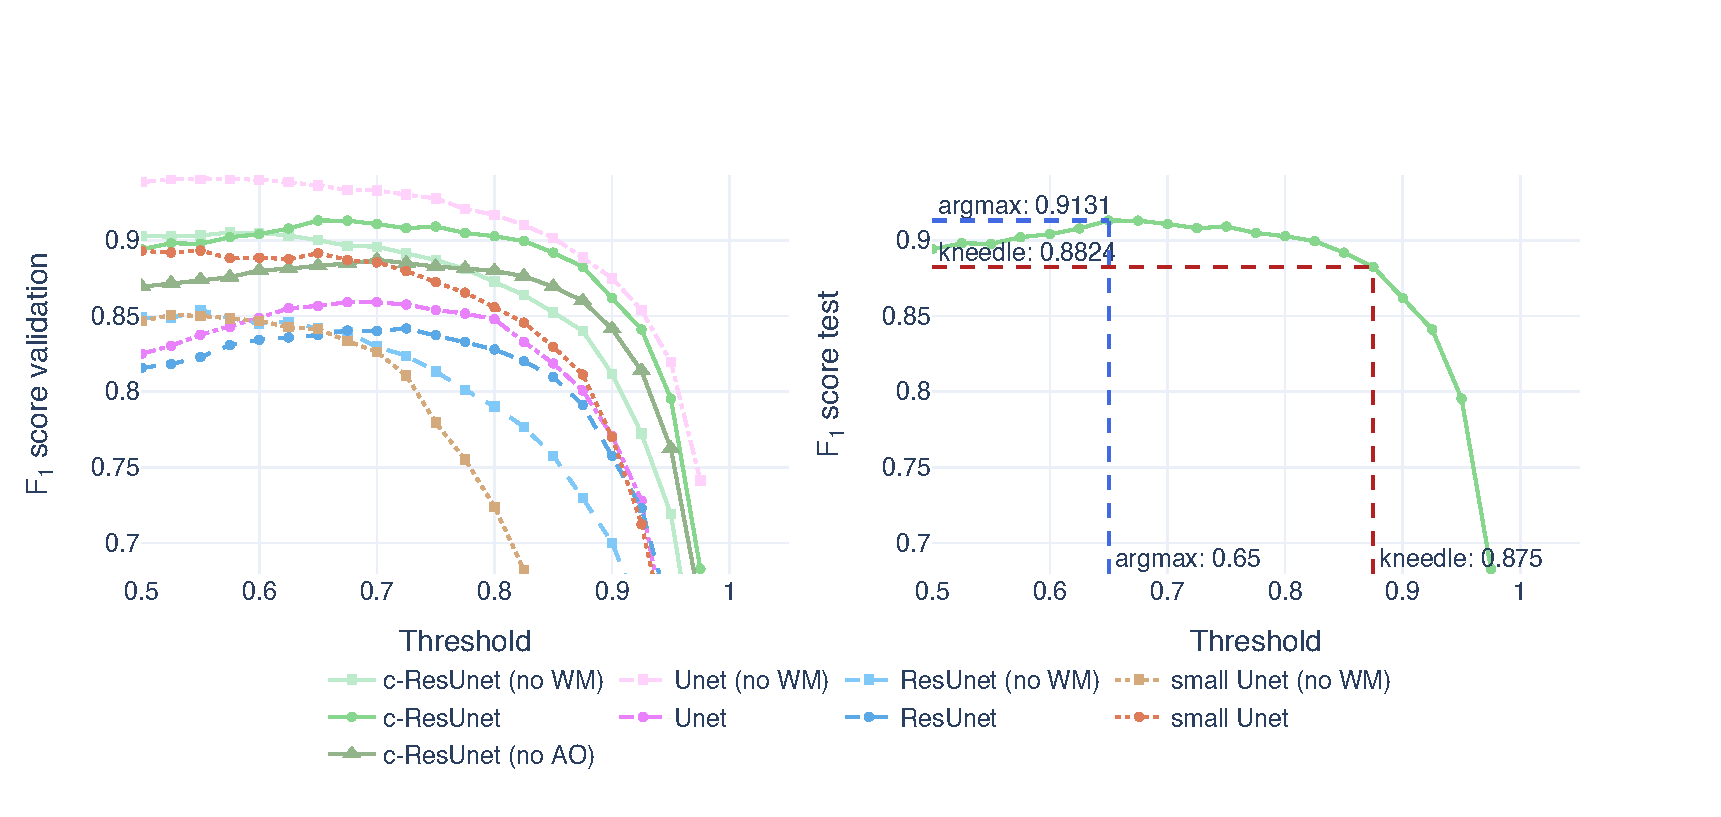
\includegraphics[width=\textwidth]{figures/130_methods/F1_optimization.eps}
}
\caption{\textbf{Threshold optimization}. On the left, the $F_{1}$ score computed on validation images as a function of the cutoff for thresholding.
On the right, the test $F_1$ score of the c-ResUnet model is used to illustrate the selection of the best threshold for binarization according to \textit{argmax} (blue) and \textit{kneedle} (red) methods.
} 
\label{fig:thresh_opt}
\end{figure}
% If the distance between their centroids was less than a fixed threshold (50 pixels, i.e. average cell diameter), the predicted element was considered a true positive; a false negative otherwise.
% Detected items not associated with any target were considered as false positives instead.

\Cref{fig:thresh_opt} shows the optimization results. On the left, we can see how each model performance varies in the validation set as a function of the cutoff for binarization.
For the adaptive thresholding approach, only very high thresholds lead to acceptable performances and we observe a sharp peak followed by a rapid decrease thereafter.
% Even though lower thresholds work best for all DL models, the $F_1$ curves are rather flat after their peaks. 
On the contrary, all DL models work best for lower thresholds and present $F_1$ curves which are rather flat after their peaks.
Thus, increasing the cutoff allows focusing only on predictions whereby the model is very confident, with just a slight loss in overall performance.
Also, good practices in natural science applications suggest being conservative with counts and only consider clearly stained cells.
For these reasons, we opted for the \textit{argmax} value (0.994) for the baseline approach, while we resorted to the \textit{Kneedle} method \cite{kneedle} for the selection of the optimal DL threshold. 
An example of that choice in the case of c-ResUnet is reported in \cref{fig:thresh_opt} (right).
% \chapter{Results}
\label{chap:partI_results}

After the training, the four competing architectures were compared in three different scenarios: full design, weight maps only (no AO) and artifacts oversampling only (no WM). 
The 70 full-size images of the test set were used as a testbed.
Table \ref{tab:metrics} reports individual model performances in terms of both detection and counting ability.
\begin{table}[H]
\begin{center}
{
\begin{tabular}{lrrrrrrrr}
\toprule
Model &  Threshold &      $F_1$ &  Accuracy &  Precision &  Recall &     MAE &  MedAE &     MPE \\
\midrule
\textbf{c-ResUnet}          &      \textbf{0.875} &  \underline{\textbf{0.8149}} &    \textbf{0.6877} &     0.9081 &  \textbf{0.7391} &  \underline{\textbf{3.0857}} &    \textbf{1.0} & -0.0513 \\
c-ResUnet (no AO)  &      0.875 &  0.8047 &    0.6732 &     0.9019 &  0.7264 &  3.0857 &    1.5 & -0.0624 \\
c-ResUnet (no WM)  &      0.875 &  0.7613 &    0.6147 &     0.9418 &  0.6389 &  3.6857 &    \textbf{1.0} & -0.1914 \\
\midrule
ResUnet            &      0.850 &  0.7855 &    0.6468 &     0.8865 &  0.7052 &  3.3286 &    \textbf{1.0} & \textbf{-0.0484} \\
ResUnet (no WM)    &      0.850 &  0.7513 &    0.6016 &     0.9387 &  0.6262 &  4.0571 &    2.0 & -0.2412 \\
Unet               &      0.875 &  0.7724 &    0.6291 &     0.9117 &  0.6700 &  3.5143 &    1.5 & -0.1436 \\
Unet (no WM)       &      0.850 &  0.7886 &    0.6510 &     0.8989 &  0.7024 &  3.1571 &    2.0 & -0.0923 \\
small Unet         &      0.875 &  0.7563 &    0.6081 &     0.9264 &  0.6389 &  3.5714 &    2.0 & -0.2137 \\
small Unet (no WM) &      0.825 &  0.6697 &    0.5034 &     \textbf{0.9483} &  0.5176 &  4.7714 &    2.0 & -0.3201 \\
\bottomrule
\end{tabular}
\caption{
Performance metrics computed on the test set using the optimal \textit{kneed} threshold. The first four columns report the detection metrics, while the latter ones evaluate counting performance.
}
\label{tab:metrics}
}
\end{center}
\end{table}

\noindent\textbf{Performance}.
By looking at the main figures of merit ($F_1$ score and MAE), c-ResUnet clearly outperforms all competitors.
Remarkably, the Unet is consistently worse than c-ResUnet and ResUnet despite having far more parameters (nearly 14M against 1.7M and 887k, respectively).
The advantage of the ResUnet architectures is even more evident when comparing with the lighter Unet version which has a comparable number of parameters (876k).

In addition, c-ResUnet keeps its leading role also when extending the evaluation to the other metrics.
The only meaningful exception is precision, for which the Unet architectures are better. This is probably due to a tendency to "overdetection". 
Nonetheless, the ResUnet counterparts well balance this behaviour with a significant improvement in accuracy and recall.

Finally, it is worth noticing that adopting the kneed optimal threshold ensures large cutoffs and enforces only detections with high confidence.
Although desired, this behavior also increases false negatives as less cells are detected. 
As a result, we observe a drop in the accuracy whereby the impact of false negatives is twice as much the one in the $F_1$ score (cfr. Eq. \eqref{eq:accuracy} and Eq. \eqref{eq:F1}), thus explaining the gap between these two metrics.
% As a result, we observe a drop in the measures that are more impacted by false negatives, which explains the lower value of the accuracy compared to the $F_1$ score.
In conclusion, the model provides reliable predictions and satisfies the design requirement of being conservative with counts, as suggested by the negative values of MPE for all experimental conditions.

\noindent\textbf{Ablation studies}.
In order to evaluate the impact of artifacts oversampling and weight maps, the experiments were repeated under the same conditions
% described in \nameref{sec:model_training}
, alternately switching off one of the two design choices.

From Table \ref{tab:metrics} it is evident how penalizing errors in crowded areas has a positive impact. Indeed, experiments exploiting weight maps achieve consistently better results than those without this addition (no WM), except for the Unet architecture.  
In particular, this strategy seems to produce a loss in precision to foster a more significant gain in accuracy and recall.
Fig. \ref{fig:weigths_effect} illustrates a visual comparison of c-ResUnet output in crowded areas with (top) and without (bottom) weight maps. 
Again, its beneficial contribution is apparent, with close-by cells sharply separated when exploiting the weight maps.

Regarding the impact of artifacts augmentation, Table \ref{tab:metrics} shows how there is little difference between the full c-ResUnet and the one without oversampling of challenging examples (no AO).
In particular, the advantage of artifacts oversampling is numerically minimal.
This is also confirmed by qualitative evaluation (Fig. \ref{fig:predictions}).
On the one hand, the c-ResUnet (no AO) is able to avoid detecting more evident artifacts as the strip (\ref{fig:predictions:noAO}) even without specific oversampling.
On the other, the c-ResUnet  still fails to ignore more troublesome bright structures (\ref{fig:predictions:artifact}) although additional challenging examples were provided during training.
For this reason, the experiment was not replicated for the other architectures. 
\begin{figure}
% \begin{wrapfigure}{R}{0.55\textwidth}
\centerline{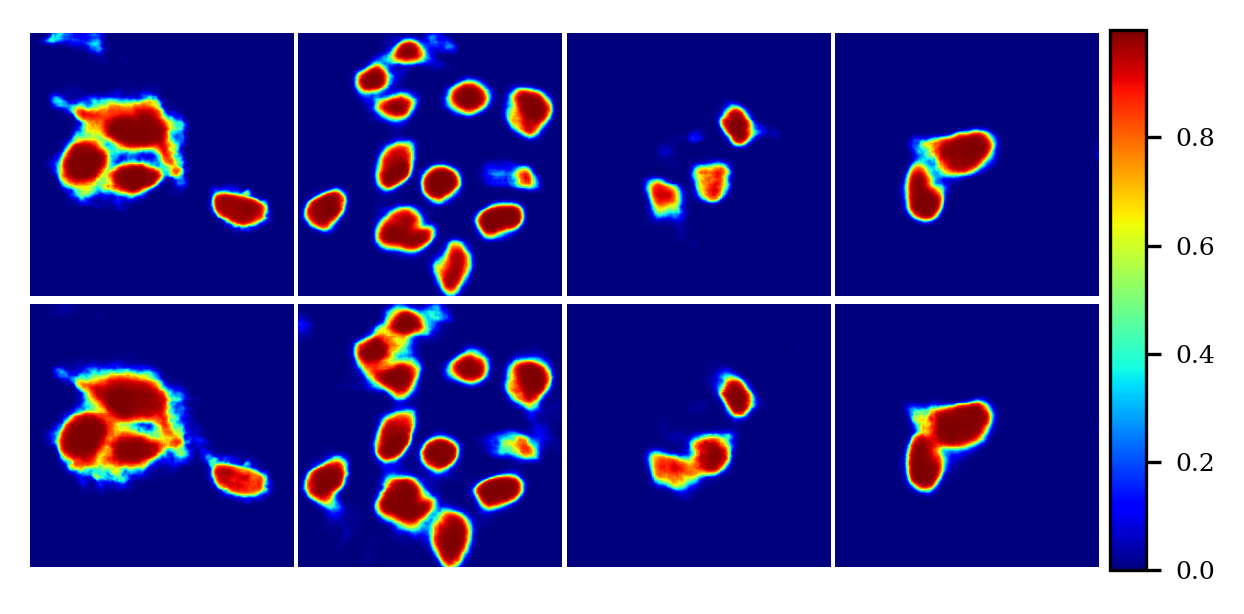
\includegraphics[width=0.8\textwidth]{figures/130_methods/weigths_effect.png}}
\caption{\textbf{Weight map effect}. 
Predicted heatmaps obtained with c-ResUnet (top row) and c-ResUnet (no WM).} 
\label{fig:weigths_effect}
% \end{wrapfigure}
\end{figure}
\begin{figure}
\centerline{
     \begin{subfigure}[]{0.52\textwidth}
         \centering
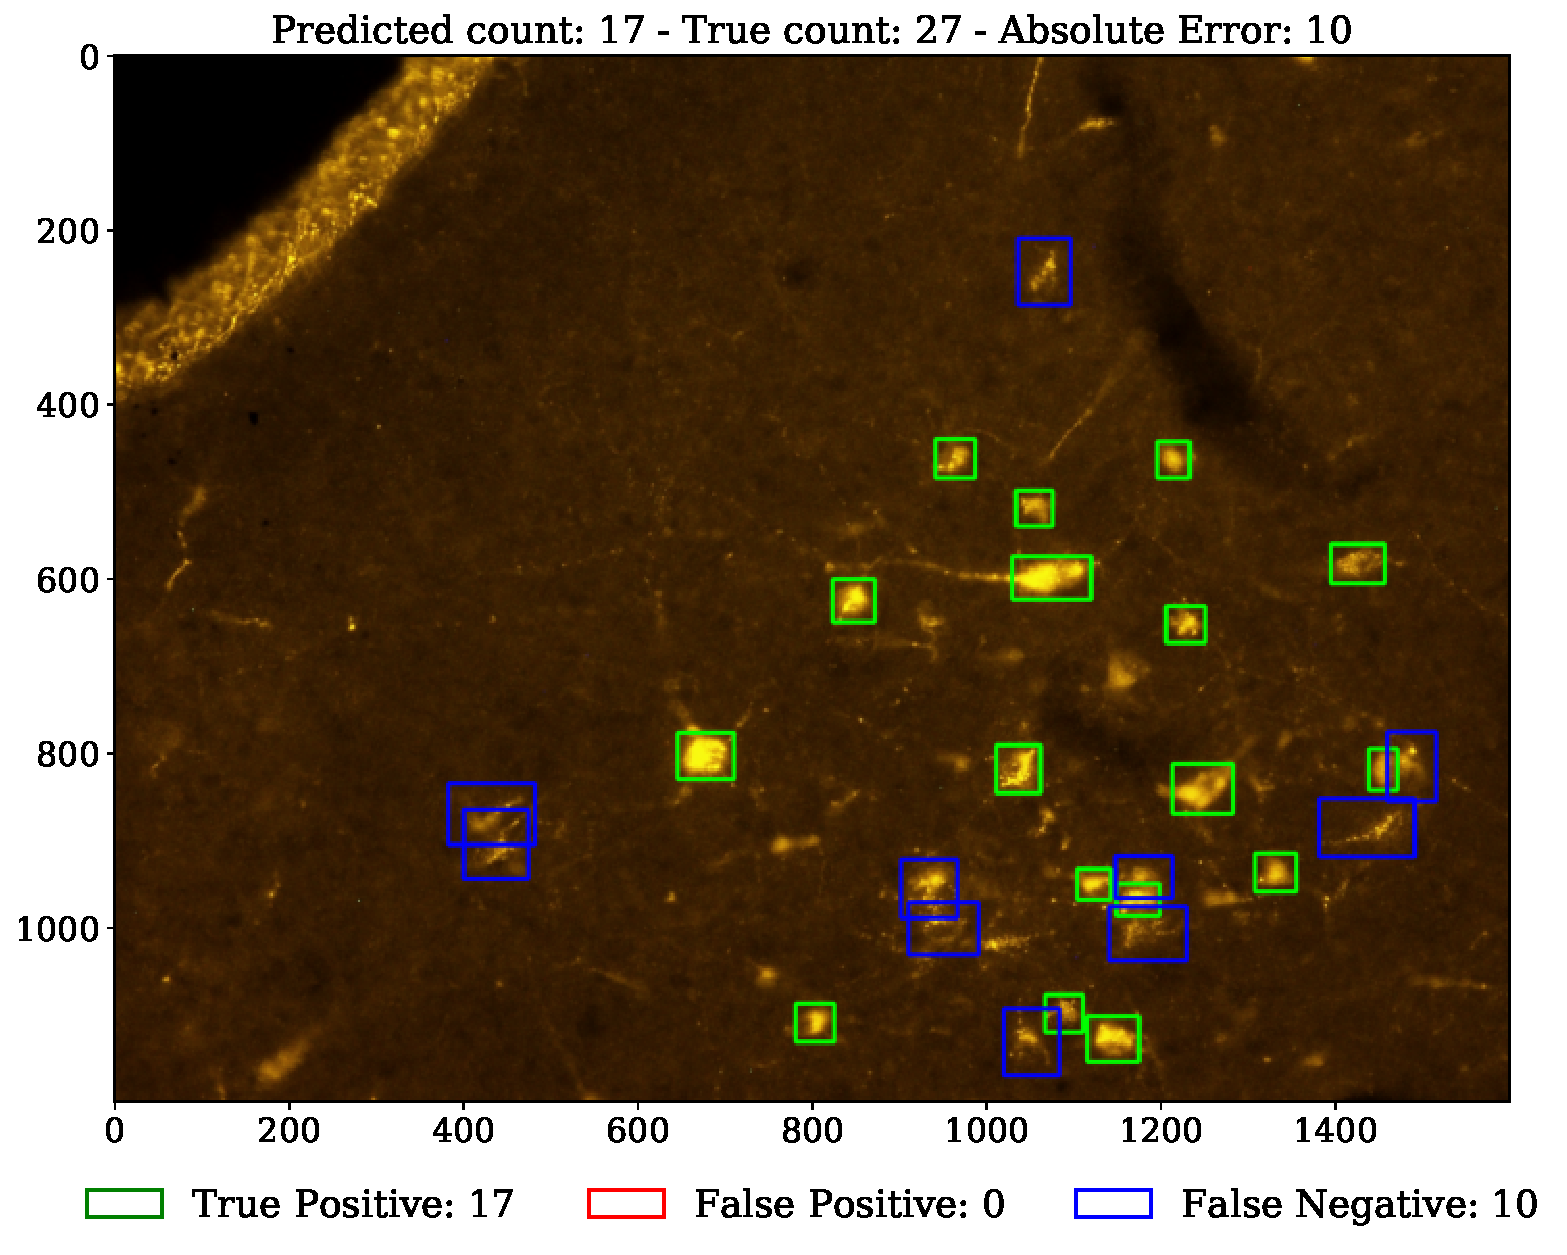
\includegraphics[width=\textwidth]{figures/140_results/pred_ResUnet_noAO:281.eps}
        \caption{
        % c-ResUnet (no AO) prediction on artifact
        }
        \label{fig:predictions:noAO}
     \end{subfigure}
          \begin{subfigure}[]{0.52\textwidth}
         \centering
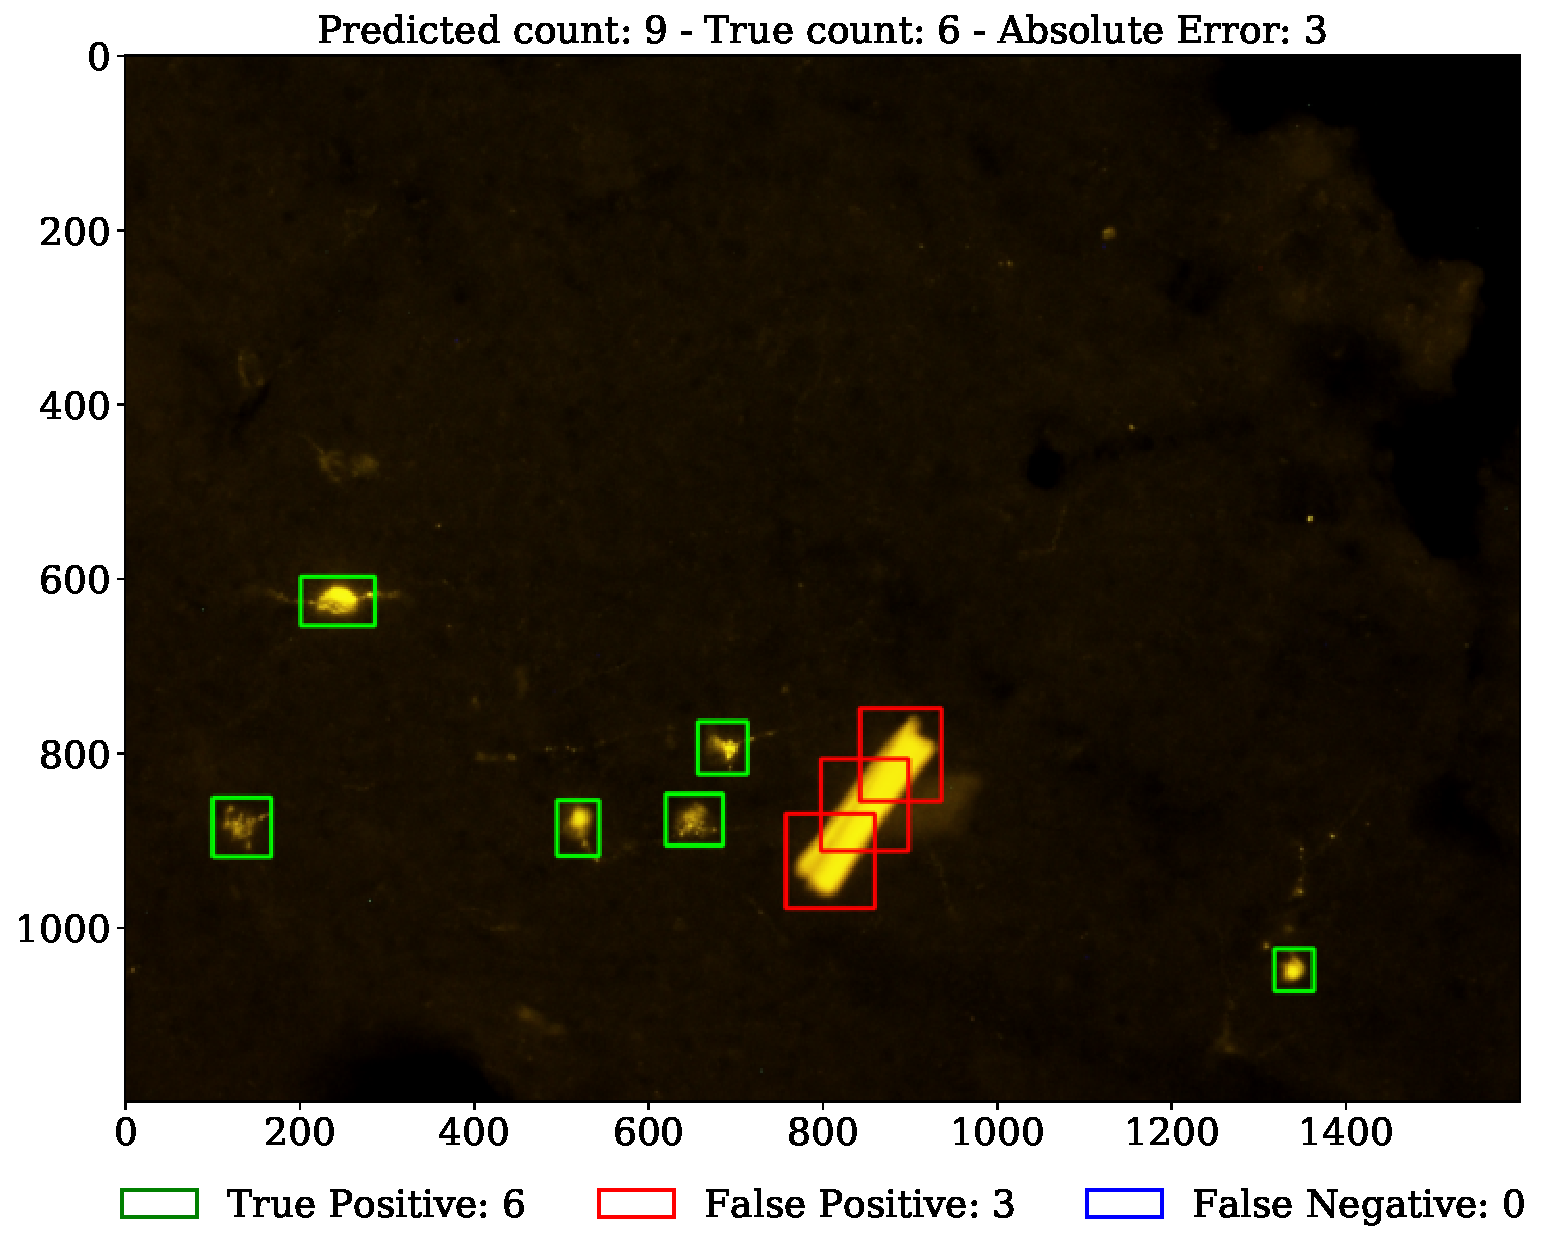
\includegraphics[width=\textwidth]{figures/140_results/pred_ResUnet:254.eps}
        \caption{
        % c-ResUnet prediction on artifact
        }
        \label{fig:predictions:artifact}
     \end{subfigure}
}
\centerline{
          \begin{subfigure}[]{0.52\textwidth}
         \centering
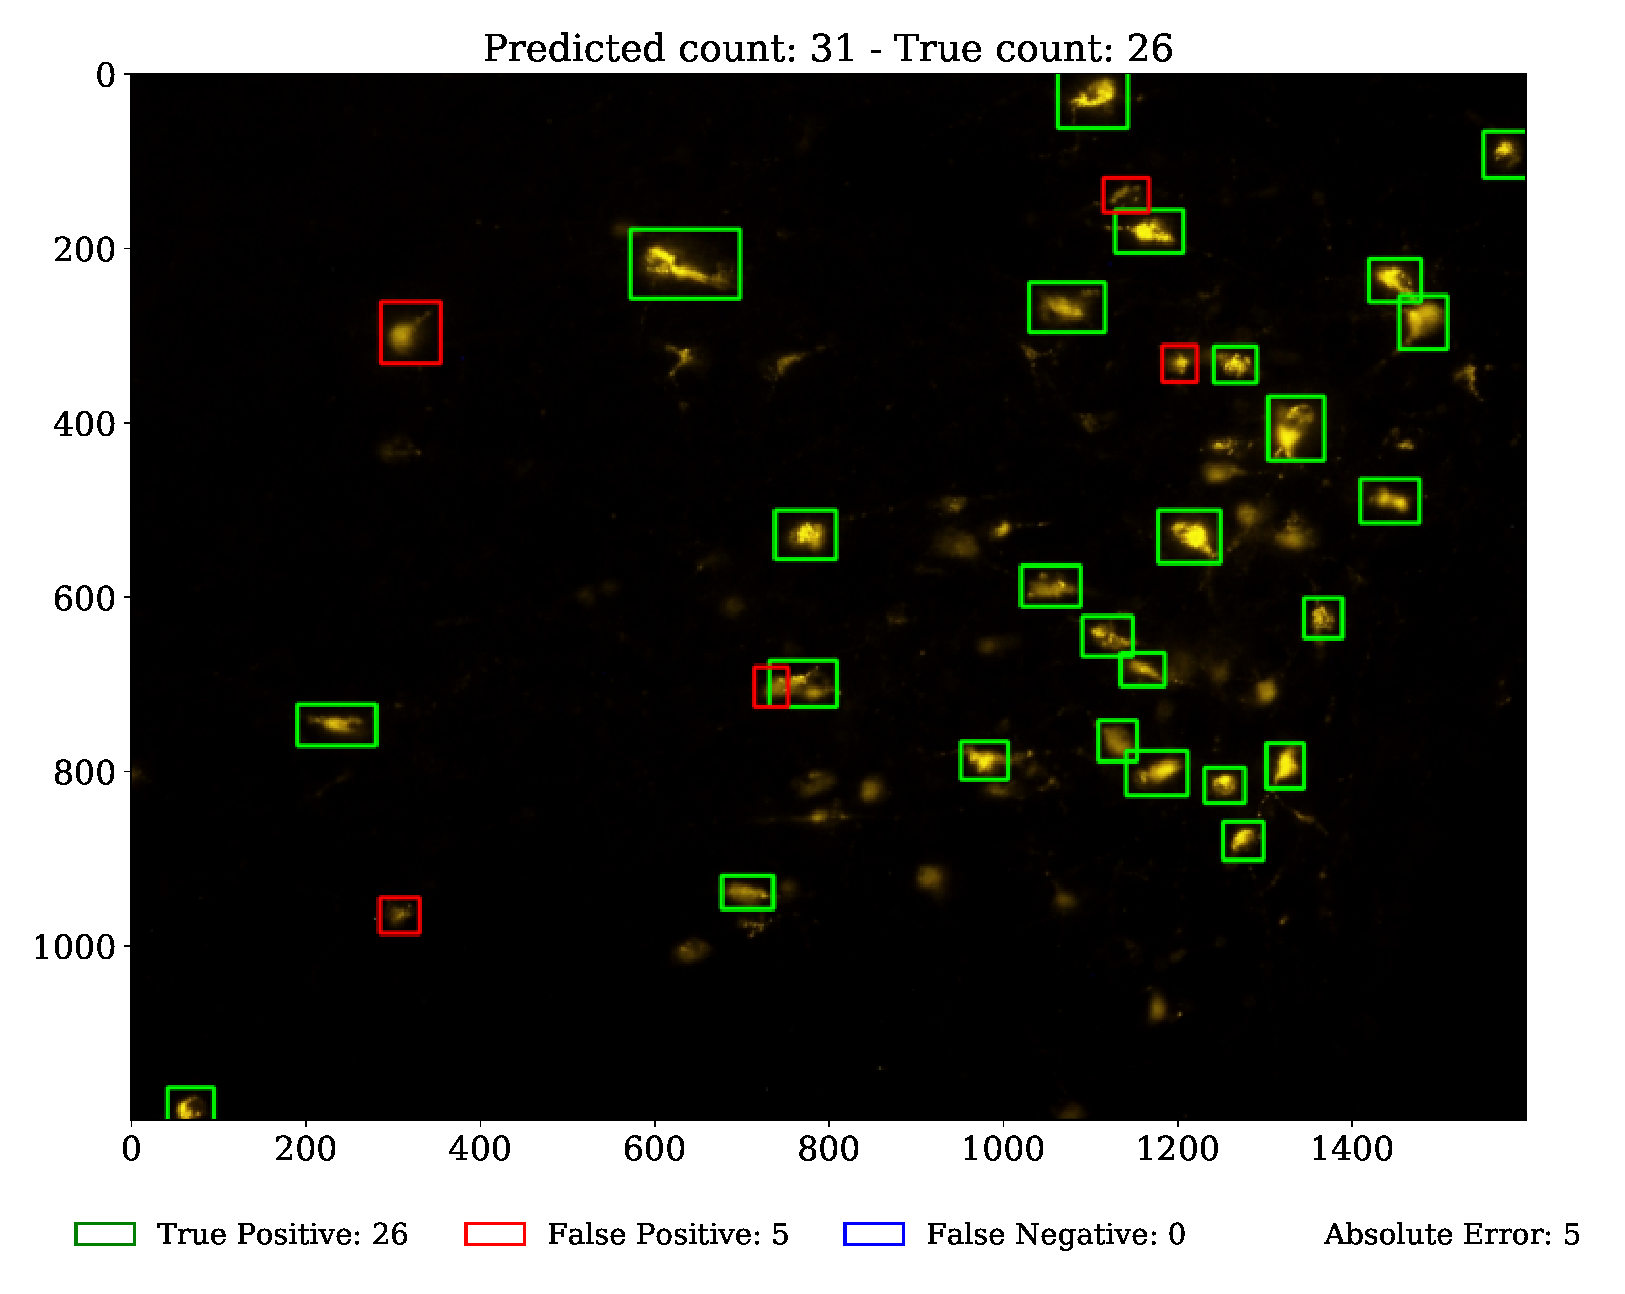
\includegraphics[width=\textwidth]{figures/140_results/pred_ResUnet:168.eps}
        \caption{
        % c-ResUnet prediction on artifact
        }
        \label{fig:predictions:false-positives}
     \end{subfigure}
       \begin{subfigure}[]{0.52\textwidth}
         \centering
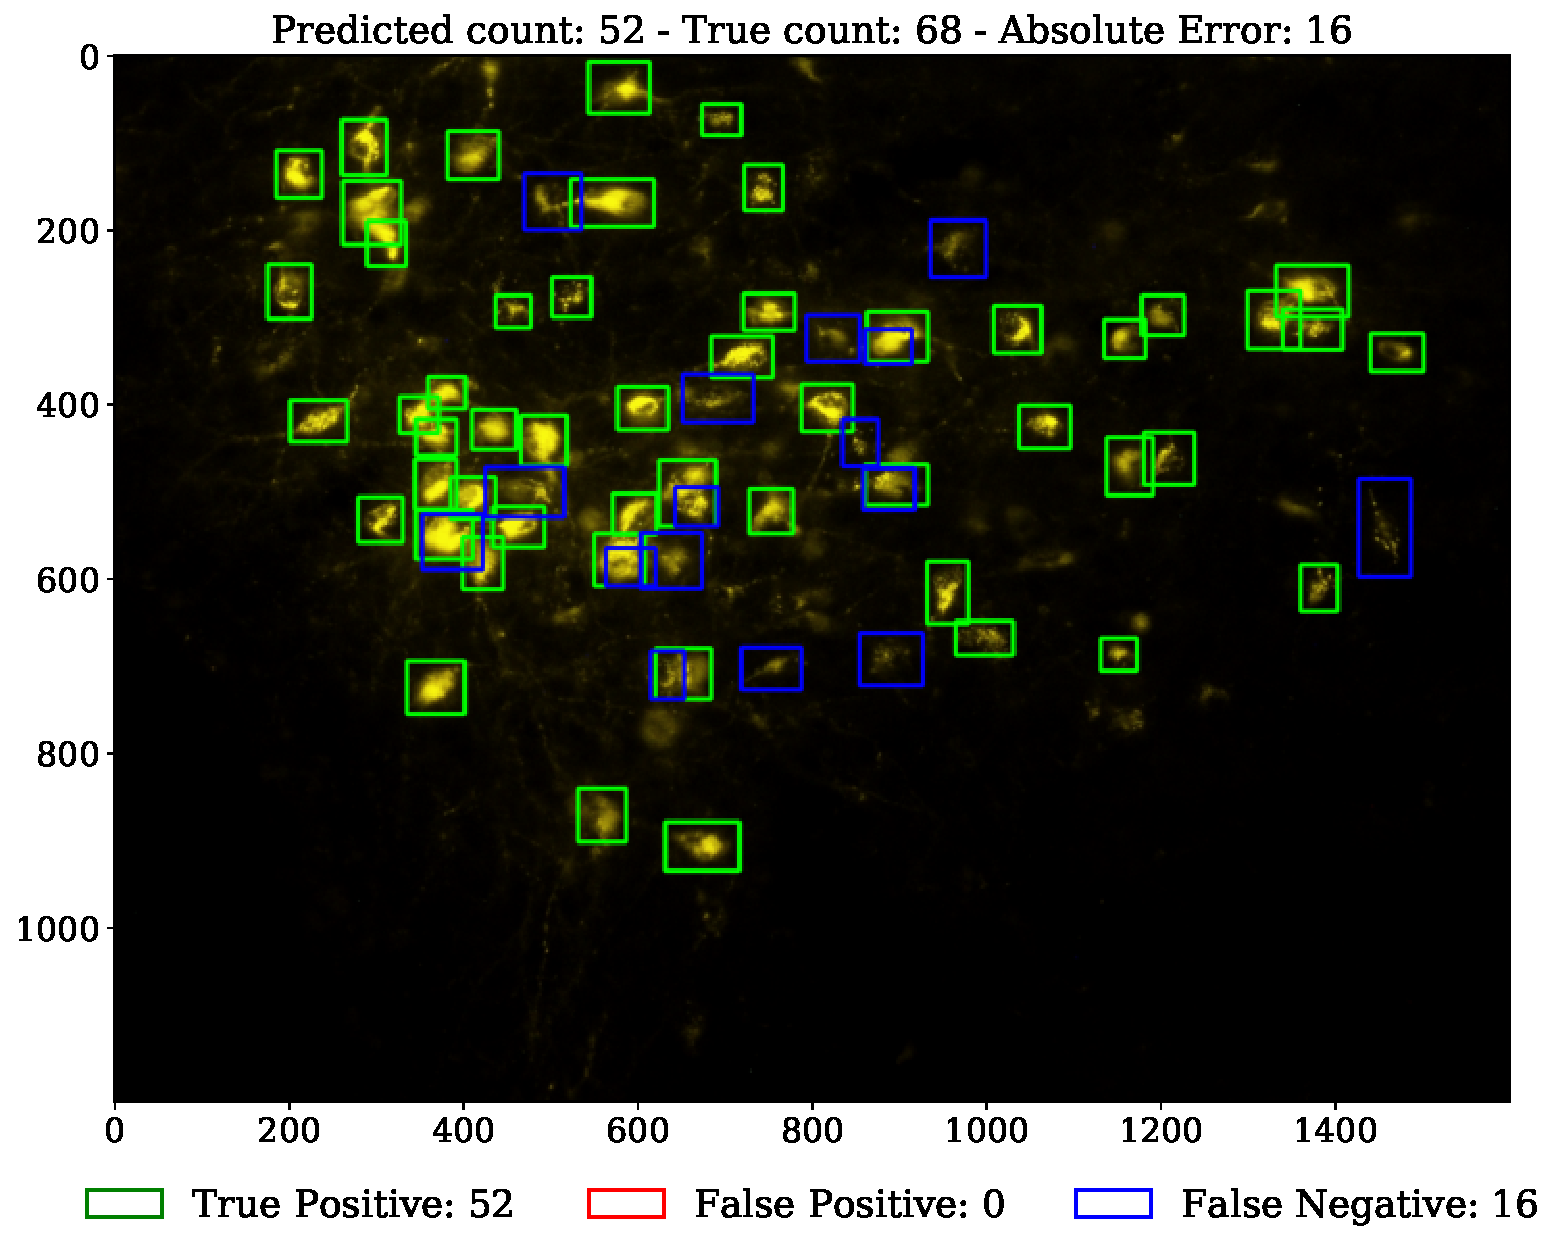
\includegraphics[width=\textwidth]{figures/140_results/pred_ResUnet:278.eps}
        \caption{
        % c-ResUnet prediction on artifact
        }
        \label{fig:predictions:false-negatives}
     \end{subfigure}
}
\caption{\textbf{Results on test images}. 
% Top row illustrates AO effect. 
The c-ResUnet (no AO) correctly handles evident artifacts (\ref{fig:predictions:noAO}, top left corner), while the c-ResUnet fails with more problematic structures (\ref{fig:predictions:artifact}).
% Bottom row highlights c-ResUnet predictive ability. 
Notice how false positives (\ref{fig:predictions:false-positives}, red boxes) look like target cells. Likewise, the objects discarded (\ref{fig:predictions:false-negatives}, blue boxes) are similar to other stains that were not annotated.
} 
\label{fig:predictions}
\end{figure}
% \chapter{Conclusions}
\label{chap:partI_conclusions}
In \cref{partI}, we tackled the issue of automating counting cells in fluorescent microscopy images through the adoption of Deep Learning techniques.

From the comparison of four alternative CNN architectures, the cell ResUnet (c-ResUnet) emerges as the best model amongst the investigated competitors.
Remarkably, the careful additions with respect to the ResUnet \cite{deep_resunet} -- i.e. a learned colorspace transformation and a residual block with 5$\times$5 filters-- enable the model to perform better than the original Unet \cite{unet} despite having seven times fewer parameters.

Also, the two design choices considered in the ablation studies provide an additional boost in model performance. 
On one side, the adoption of a weight map that penalizes errors on cell boundaries and crowded areas is definitely helpful to promote accurate segmentation and dividing close-by objects. 
On the other, the effect of artifacts oversampling is less evident.
Nonetheless, the combined impact of the two components guarantees better results than any of the two considered separately.

In terms of overall performance, the results are satisfactory. 
Indeed, the model predicts very accurate counts (\mbox{MAE = 3.0857}) and satisfies the conservative counting requirement, as testified by the negative MPE (-5.13\%).
Detection performance is also very good (\mbox{$F_1$ score = 0.8149}), certifying that the precise counts come from accurate object detection rather than a balancing effect between false positives and false negatives.

Finally, qualitative assessment by domain experts corroborates further the previous statements. 
Indeed, by visually inspecting the predictions is possible to appreciate how even erroneous detections are somewhat arguable and lay within the subtle limits of subjective interpretability of borderline cases (see \cref{fig:predictions:false-positives,fig:predictions:false-negatives}).


In conclusion, the proposed approach proved to be a solid candidate for automating current operations in many use cases related to life science research.
Thus, this strategy may bring crucial advantages in terms of speeding up studies and reducing operator bias both within and between experiments.
For this reason, by releasing the c-ResUnet model\footnote{\linkmodel} and the annotated data\footnote{\dataset}, we hope to foster applications in microscopic fluorescence and similar fields, alongside innovative research in Deep Learning methods.
\part{Second Part}
\label{partII}

% \chapter{Contribution}

% You may also put some code snippet (which is NOT float by default), eg: \cref{lst:random-code}.

% \lstinputlisting[float,language=Java,label={lst:random-code}]{listings/HelloWorld.java}
% \label{lst:random-code}

% \cref{lst:metrics-code}.

% \lstinputlisting[float,language=python,label={lst:metrics-code}]{listings/metrics.py}
% \section{Fancy formulas here}

\chapter{Introduction}

% We are witnessing an ever-increasing trend in data production, thus leading to the so-called \emph{Big Data} era. 
% \note[Luca][notesyellow]{Espandere descrizione con esempi e brevi cenni storici}

In the last twenty years, we have witnessed an unprecedented and ever-increasing trend in data production. 
\citeA{hilbert2011world} date the rise of this phenomenon back to 2002, with the beginning of the digital age.
Indeed, the transition from analog to digital storage devices enormously expanded the capacity of accumulating data, thus leading to the \emph{Big Data} era.

The term big data was first introduced in 1990s \cite{16, 17} and it is commonly adopted to describe datasets whose size exceeds the potential to manipulate and analyze them within reasonable time limits \cite{snijders2012big}.
However, the expression does not target any specific storage size but rather assumes a deeper meaning that goes well beyond the sheer amount of data points.
In fact, big data embrace a broad spectrum of data sources including structured, semi-structured and, mostly, unstructured data \cite{dedic2016towards}.
Although multiple connotations have been attributed to the concept of big data over the years, a commonly shared definition is related to the so-called \emph{5 Vs} \cite{3}:

\begin{itemize}
    \item \textbf{Volume}: the actual quantity of generated data is huge, in the order of magnitude of terabytes and petabytes \cite{sagiroglu2013big}. More generally, it indicates amounts that are too large and complex to exploit conventional data storage and processing technologies;
    
    \item \textbf{Variety}: the data may come in several data types and from diverse origins. These include sources as sensors, social media, log files and more, plus they encompass heterogeneous formats like text, images, audio, video and so on; 
    
    \item \textbf{Velocity}: data are produced and/or processed at high rates \cite{kitchin2016makes}, typically nearly real-time;
    
    \item \textbf{Value}: data must carry valuable information that, if correctly analyzed, bring business value and profitable insights \cite{uddin2014seven}. In a scientific context, this means information that contribute to the advancement of human knowledge;
    
    \item \textbf{Veracity}: data sources must be reliable and generate high-quality data that can produce value \cite{onay2018review, 33};


\end{itemize}


Nonetheless, the community has not reached a complete agreement on the big data definition \cite{22, kitchin2016makes}, with some authors suggesting moving their characterization from the intrinsic properties to the techniques adopted to acquire, store, share and analyze the data \cite{balazka2020big}.


Besides the modification of the storage supply,  multiple factors significantly enhanced data production and, hence, favored the rise of the big data era.
% the demand for storage space and computing power.
In the first place, the diffusion of the internet and the progress of computer technologies provided more processing capabilities and easier access to data, thus stimulating further their production.
Consequently, several stakeholders as big tech companies, traditional industries, governments, healthcare institutions and more started increasingly contributing to this growth.
Finally, the introduction of \emph{smart} everyday objects that not only receive but also produce data exponentially accentuated individual contributions to the total data produced.
Modern objects, in fact, are endowed with technologies that allow to collect data and share them via a network -- the so-called Internet of Things \cite{ashton2009iot} --, thus augmenting the production rate even more.
For instance, sensors measuring the status and operation are now commonly used in industrial machinery and household appliances to ease their control and automate maintenance.
The same paradigm is also influencing the direction of the personal items market in various ways.
% and, in turn, new use-cases emerge from their adoption. 
For example, some tech companies are recently investing in wearable devices like watches and glasses to enable the users to be always connected with a rapidly mutable environment, track their progress and explore the world in unparalleled manners thanks to virtual reality.
Furthermore, the solutions that digitization offers are being explored to respond to the emerging challenges of current times.
Think, for instance, of the urge for modernization of institutional processes posed by the pandemic. The massive spread of the infections has required unprecedented amounts of patients needing access to health assistance. However, the impossibility to scale up services and equipment correspondingly caused huge issues and jeopardized people's safety. In such context, the availability of intelligent systems capable of remotely monitoring patients' conditions and providing them with specialist support would have enormously helped.

In order to cope with the growing amount of data to store and process, the big data players of both industry and academy have gradually moved to new computing paradigms in recent years. 
For instance, new solutions as \textbf{distributed} and \textbf{cloud computing} \cite{kshemkalyani2011distributed, wang2010cloud} have been specifically designed to address these new requirements, taking advantage of multiple resources geographically displaced and accessible via a network.

However, the boost in performance guaranteed by these technologies comes with the price of requiring very complex interactions of both hardware and software components. 
Aside from the enormous benefits these solutions bring, their most relevant drawback is that the wider the infrastructure, the higher the chances of something going wrong, and the bigger the effort to detect, inspect and solve the issues.
\Cref{partII} explores this domain and tries to propose a data-driven pipeline to ease and support people working to maintain the infrastructure integrity.
Despite applying to many different applications with some tuning, the presented approach is discussed in the context of \textbf{data transfer failures} within the \emph{Worldwide Large Hadron Collider Computing Grid} (WLCG).

\section{Background}
\begin{figure}
    \centering
    \subfloat[LHC accelerator]{
    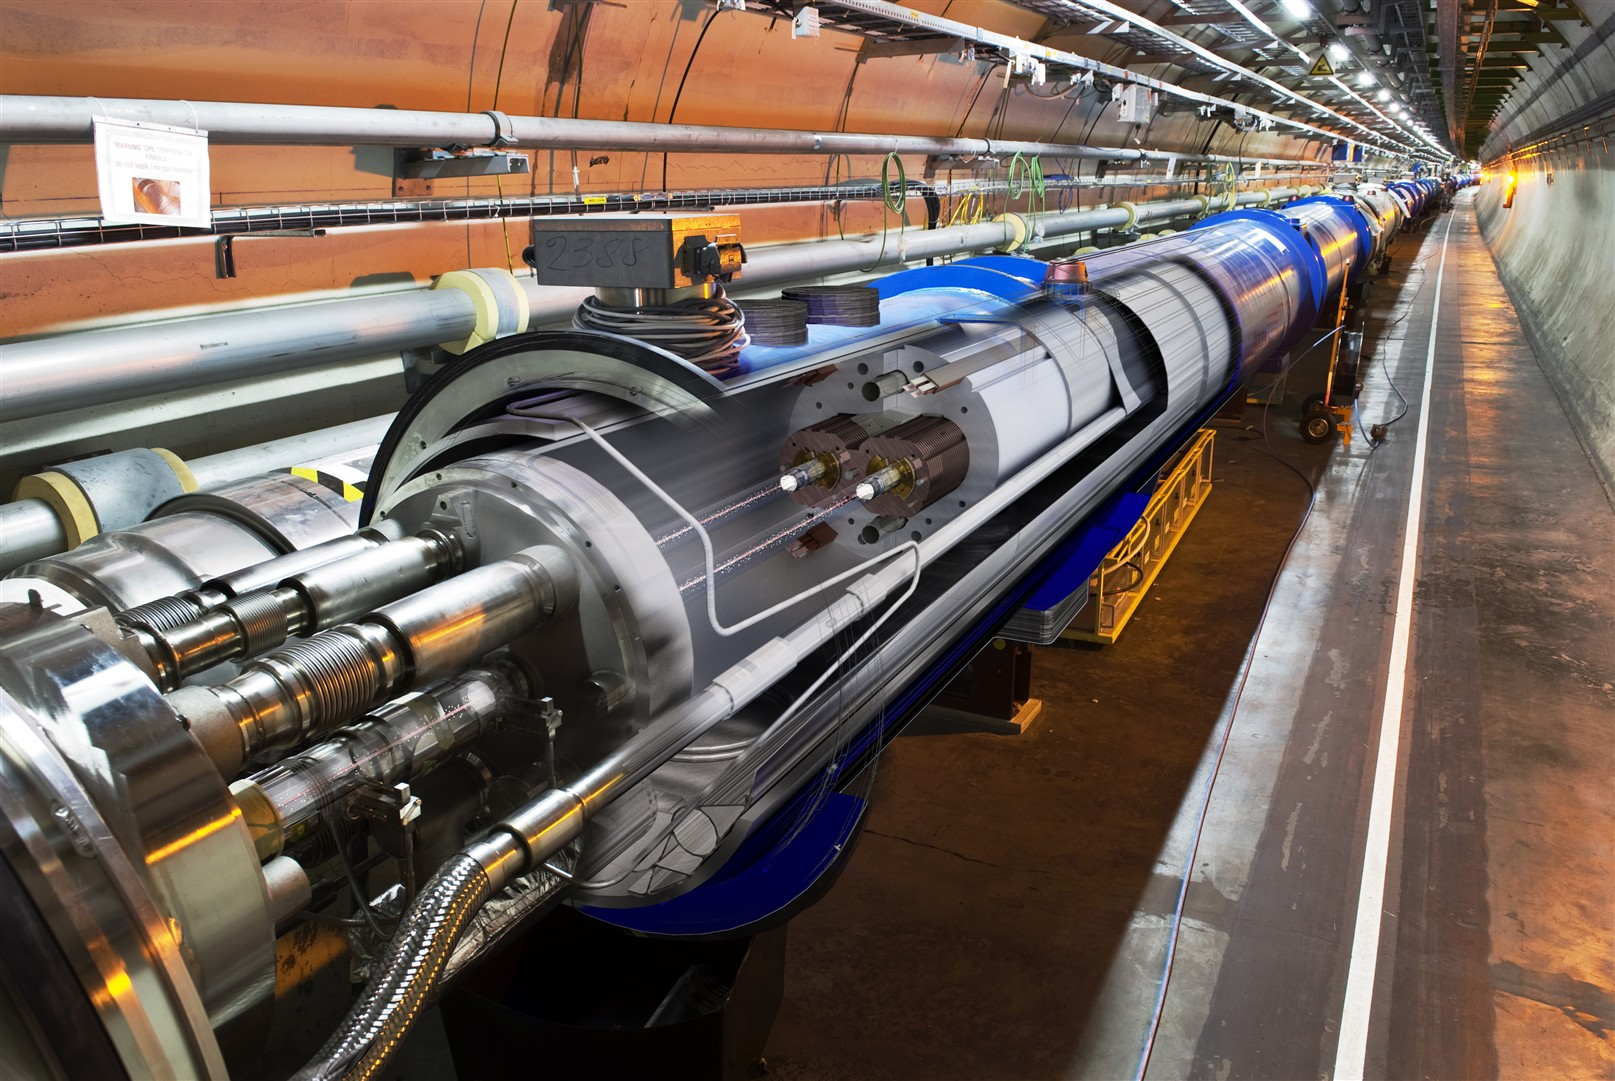
\includegraphics[width=\textwidth]{figures/220_introduction/cern/a0lhcinternotubo_445034351.jpg}
    }
    
    \subfloat[Aerial view]{
    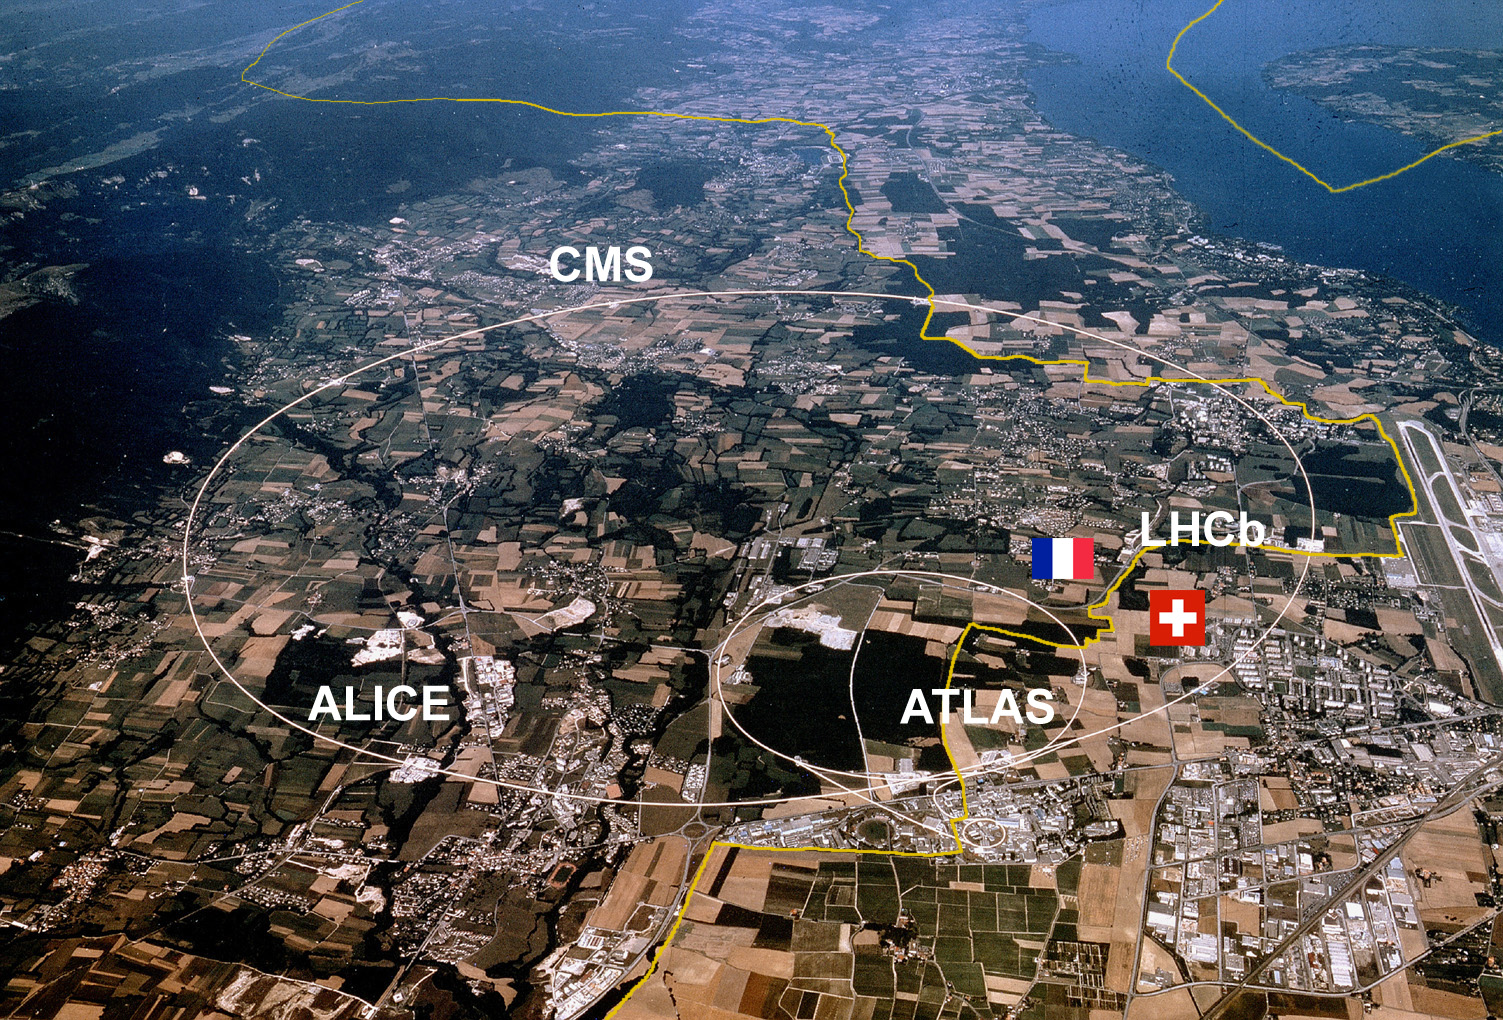
\includegraphics[width=0.5\textwidth]{figures/220_introduction/cern/CERN_location.jpg}
    }
    \subfloat[LHC scheme]{
    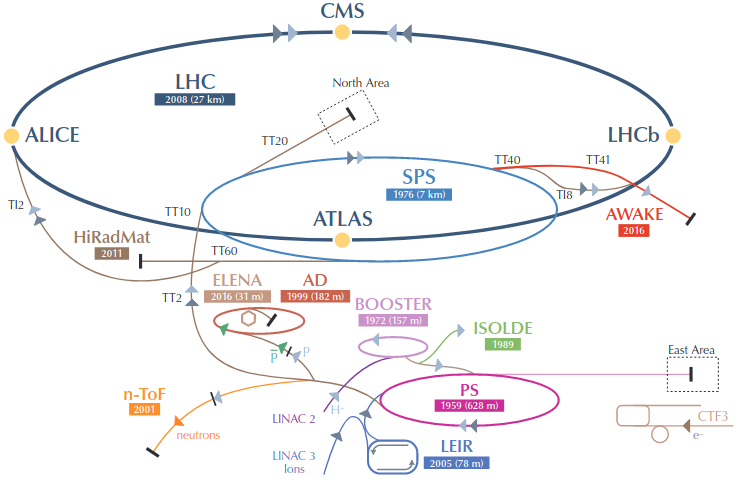
\includegraphics[width=0.5\textwidth]{figures/220_introduction/cern/lhc_scheme_factsfigures.png}
    }
    \caption{\textbf{LHC accelerator complex.} Top: the underground tunnel that hosts LHC and a transversal section of the pipes that compose it. 
    Bottom: aerial view of LHC complex at the boundary between Switzerland and France (left) and structure of the various accelerating structures that compose LHC (right).
    }
    \label{fig:lhc}
\end{figure}

\begin{figure}
    \centering
    \subfloat[ATLAS]{
    \includegraphics[width=0.5\textwidth]{figures/220_introduction/cern/atlas_detector_medium.jpg}
    }
    \subfloat[LHCb]{
    \includegraphics[width=0.5\textwidth]{figures/220_introduction/cern/lhcb_detector_medium.jpg}
    }
    
    \subfloat[ALICE]{
    \includegraphics[width=0.5\textwidth]{figures/220_introduction/cern/alice_detector_medium1.jpg}
    }
    \subfloat[CMS]{
    \includegraphics[width=0.5\textwidth]{figures/220_introduction/cern/cms_detector_medium.jpg}
    }
    \caption{\textbf{CERN 4 major experiments.}}
    \label{fig:cern_experiments}
\end{figure}

\note[Luca][notesyellow]{Introduction to HEP community, with mention to WLCG as an essential tool to perform their research}

% High-Energy Physics (HEP) is a branch of physics that studies the fundamental constituents of matter and the forces that drive their interactions. One of the methods is to create very high energy densities. 
% This reproduces the environmental conditions of the primordial universe.

High-Energy Physics (HEP) is a branch of physics that studies the elementary constituents of matter and the fundamental principles that govern their interaction to understand how our universe has formed and evolved.  
These particles, however, are not visible at the scales whereby we experience reality today. 
Thus, HEP experiments need to either look at natural phenomena generated in pressure and temperature conditions similar to those of the primordial universe -- like cosmic rays -- or recreate such settings artificially.

The European Council for Nuclear Research (CERN) is part of this second strand of experiments, and it constitutes the largest particle physics laboratory in the world.
From 2008, CERN facilities also include the Large Hadron Collider (LHC), the longest particle accelerator ever built.
LHC consists of a \mbox{26.7-kilometer} ring located in a tunnel about 100 meters underground in the Geneva area (\cref{fig:lhc}), and it is made of superconducting magnets with several accelerating structures \cite{lhcwebsite}.
Inside the accelerator, bunches of protons are revved up to nearly the speed of light, forming two high-energy particle beams that travel in opposite directions inside separated pipes. 
When they acquire the desired energy, the beams are directed towards dedicated interaction points where the experiments occur. %surrounded by giant detectors.
In practice, LHC hosts four major experiments built in correspondence of these locations -- ATLAS \cite{aad2008atlas}, ALICE \cite{aamodt2008alice}, LHCb \cite{alves2008lhcb} and CMS \cite{collaboration2008cms} -- and equipped with giant detectors (\cref{fig:cern_experiments}).
Once the beams get there, the two pipes cross and the particles are squeezed through substantial magnetic fields to increase their chances of colliding. 
In this way, a massive amount of energy is concentrated in an extremely tiny area, generating millions of particles at each collision.
Indeed, the high speed of the beams causes roughly 40 million crossings per second at each interaction point \cite{albrecht2019roadmap, grandi2017HEPsize}. 
\sidenote[Luca][notesyellow]{Controllare numeriche ed aggiungere reference}
When a crossing happens, an average of 60 bunch collisions -- also referred to as pileup -- are observed \cite{albrecht2019roadmap}. The particles produced by each scattering then fly around the interaction point to be eventually detected through high-technology experimental devices endowed with over 100 million electronic channels \cite{grandi2017HEPsize, aad2020channels}.
According to the latest experimental setup, this delivers 100 MegaBytes (MB) of data per collision and it would generate 40k ExaBytes (EB) every year \cite{grandi2017HEPsize}.
However, storing such a tremendous amount of data is unattainable with current technology and budget. In addition, the events of interest are typically rare, so there is actually no need to record all of the information detected by the electronic channels.
Thus, the vast majority of \emph{read-out} data from collisions is discarded straight away and the \emph{recorded} event rate is lowered to 1k crossings per second. 
As a result of this reduction, the actual acquisition rate
% amounts to 1MB every second, translating to roughly 100 PetaBytes (PB) a year in 2018 \cite{grandi2017HEPsize, altre?}.
amounts to nearly 1 PB per day \cite{cern2017storage}, translating to roughly 160 PetaBytes (PB)%
\footnote{LHC registered 161 days of physics data taking in 2018 \cite{todd2018lhcAvail}}
a year in 2018. %\cite{grandi2017HEPsize, cern2017datayear}.
Besides that, physics analyses require comparing experimental results with Monte Carlo data simulated according to current theories, thus producing somewhat between 1 and 2 times additional data \cite{grandi2017HEPsize}.
Furthermore, the CERN community is already working at enhancing the Large Hadron Collider capabilities.
The project involves boosting the energy of the beam and gradually increasing the pileup towards 200 collisions per bunch crossing \cite{albrecht2019roadmap}, thus leading to the so-called High Luminosity LHC (HL-LHC) \cite{hllhc}.
% Thanks to this upgrade, way more events will be observed as the beam energy will be boosted and the pileup will gradually be increased towards 150 collisions per bunch crossing.
% In this new regime, 
Thanks to this upgrade, the observed events are expected to increase of a factor $\geq5$\cite{giuspe2021tesi} and produce an estimated 800 PB of new data each year by 2026.%\cite{grandi2017HEPsize, HLLHC_data}.

Although it is difficult to replicate such a punctual measurement of the data production for other big data players, some hints can be retrieved by comparing multiple online resources. %\cite{BDPlot_series}. 
\Cref{fig:bidata_size} tries to summarize a reasonable, up-to-date ``guesstimate"%
\footnote{These data are reconstructed based on multiple online sources about the amount of contents produced, streamed or hosted by big data companies and reasonable estimates of unitary sizes for such contents, e.g. average mail or picture size, average data traffic for 1 hour video, and so on. 
However, the actual values reported are not meant to be extremely accurate and only serve the purpose of giving an idea of the orders of magnitude of the various phenomena.
}
of yearly data production for the main big data companies.
Despite not being the most popular among the mainstream audience, the HEP community is one of the most prominent players concerning big data.
% \begin{landscape}
% \begin{figure}
%     \centering
% \begin{tikzpicture}%[shorten >=1pt,node distance=1cm,on grid,auto] 
% \linespread{.5}%
% \begin{scope}
%     \node[anchor=south west,inner sep=0] (image) at (0,0){\includegraphics[width=\linewidth]{figures/220_introduction/BigData2021.pdf}};
% \begin{scope}[x={(image.south east)},y={(image.north west)}]
%     \node [anchor=west] (note1) at (0.26,0.170) {\href{https://stackoverflow.com}{Link}};
%         \node [anchor=west, scale=1, align=center,font=\tiny] (note2) at (0.26,0.470) {\href{https://rdcu.be/cB1Ds}{paper} \\ from the future};
% \end{scope}
%     \end{scope}
% \end{tikzpicture}
% \caption{\textbf{Big Data sizes.} Bubble plot of the orders of magnitude of data produced by important big data players. The balloon areas illustrate the amount of data and the text annotations highlight the key factors considered in the estimates. Average per-unit-sizes are reported in parentheses, where italic indicates measures reconstructed based on likely assumptions because no references were found.} \label{fig:bidata_size1}
% \end{figure}
% \end{landscape}
\begin{landscape}
\begin{figure}
    \centering
    \includegraphics[width=\linewidth]{figures/220_introduction/BigData2021.pdf}
    \caption{\textbf{Big Data sizes.} Bubble plot of the orders of magnitude of data produced by important big data players. The balloon areas illustrate the amount of data and the text annotations highlight the key factors considered in the estimates. Average per-unit-sizes are reported in parentheses, where italic indicates measures reconstructed based on likely assumptions because no references were found. Interactive version available at: \href{https://clissa.github.io/BigData2021/BigData2021.html}{BigData2021.html}}
    \label{fig:bidata_size}
\end{figure}
\end{landscape}

Indeed the read-out data LHC produced every year in Phase 2 (40k EB) is around one order of magnitude bigger than the total size of objects ever stored on Amazon AWS cloud service (500 EB)%
\footnote{Obtained considering the total number of objects reportedly stored in Amazon S3 (100 trillion, \citeA{amazon2021objectscount}) and assuming an average size of 5 MB based on some average bucket example \cite{amazon2021objectssize}}.
Considering effectively recorded data, LHC figures are comparable with those of other most renowned big data entities. The last run (2018), in fact, produced hundreds of PetaBytes (PB) (roughly 160 of real data and 240 of Monte Carlo simulations),
 which is similar to the orders of magnitude generated by Google searches (62 PB)%
\footnote{Obtained considering that Google search index contains at least 30 billion webpages \cite{van2016estimating, google2021index_size, djuraskovic2020googl_stats, indig2020index_size} and that the average page size is 2.07 MB \cite{http2021webpage_size}
},
Instagram and Facebook shared photos (68 and 252 PB, respectively)%
\footnote{Obtained considering that 65k and 240k pictures are shared every minute on Instagram and Facebook \cite{domo2021infographic}, and assuming 2 MB as a reasonable average picture size \cite{adobe2021fb_img_size}
}
and YouTube video uploads (263 PB)%
\footnote{Obtained considering that 720k hours of video are uploaded daily \cite{domo2021infographic} and assuming an average size of 1 GB \cite{quora2021youtube}
}.
Moreover, LHC will climb the table even further with the upgrade to high luminosity, when the real and Monte Carlo data production rate is expected to rise to levels comparable to those of storage services like Dropbox (800, 1200 and 768 PB%
\footnote{Obtained considering that Dropbox registered 100 million of new users in 2020, of which 1.17 million were paid subscriptions \cite{dean2021dropbox}. For the average per-unit-size, it was assumed that free accounts exploited 75\% of the 2 GB storage available, while paid ones exploited 25\% of the total 2 TB
}, respectively). 

Apart from the nominal values of the generated information, streaming data comprise a significant slice of the big data market.
As a matter of fact, the continual movement of small- to medium-sized files spawns massive traffic when scaled up to millions of users, as testified by e-mails (5.7k PB)%
\footnote{Obtained considering that 71k billion e-mails and 60k billion spam messages were sent from October 2020 to September 2021 \cite{statista2021mails}, and that the average size is \mbox{75 KB} for e-mails \cite{lifewire2021avg_mail} and \mbox{5} KB for spam \cite{medium2014avg_spam}
},
and Netflix (51.1k PB)%
\footnote{Obtained considering that Netflix users consumed 140 million hours per day of streaming \cite{domo2021infographic} and that counts for 1 GB of data for standard definition videos \cite{perry2021netflix}
} bubbles in \cref{fig:bidata_size}.
% Also in this respect, LHC plays an important role. Indeed, the HEP community is formed by thousands of researchers spread around the world that need to access the data produced at CERN.
A similar usage is generated also by the LHC, whose data are continuously transferred across the HEP community thanks to the Worldwide LHC Computing Grid (see \cref{wlcg}) to fuel innovative research. For example, 
% 12 PB of data were accessed on average every day in 2020 for the ATLAS experiment alone \cite{calafiura2020design_report}, and
a throughput of 60 GB/s was generated by the 4 experiments together in 2018 \cite{wlcg2018throughput} thus giving a yearly projection (1.9k PB) close to half of the global e-mails traffic and only one order of magnitude lower than Netflix usage.
% Indeed, thousands of researchers from all around the world need to access LHC data, analyze them and share their results to investigate new theories and advance our knowledge of the universe.
% For this reason, the Worldwide LHC Computing Grid computing infrastructure has been developed over the years 

Given the large quantities of data involved by the LHC, it is not surprising how careful planning must be done in order to meet the needs of the LHC community, and tailored strategies and technologies must be adopted to cope with such requirements. 
Luckily, the presence of other stakeholders facing analogous problems provides the HEP community with some alternatives to draw from, and it allows researchers to tap in from existing solutions and customize them for their necessities.

\subsection{The Worldwide LHC Computing Grid}
\label{wlcg}

\sidenote[Luca][notesyellow]{Cos'è WLCG?}
The Worldwide LHC Computing Grid (WLCG) is a global collaboration that links up more than 170 computing centers in 42 countries. 
As of today, WLCG constitutes the largest computing grid in the world and it is supported by many associated national and international grids across the world, such as European Grid Initiative (Europe-based) and Open Science Grid (US-based), as well as many other regional grids.

Founded in 2002 by CERN, the WLCG mission is to provide computing resources to store, distribute and analyze the data generated by the Large Hadron Collider (LHC).
In order to do that, WLCG leverages a distributed computing paradigm to share resources -- in terms of infrastructures, personpower and fundings -- among member states and make them equally available to all the partners, regardless of their physical location.

WLCG is the world's largest computing grid. It is supported by many associated national and international grids across the world, such as European Grid Initiative (Europe-based) and Open Science Grid (US-based), as well as many other regional grids.

WLCG is co-ordinated by CERN. It is managed and operated by a worldwide collaboration between the experiments (ALICE, ATLAS, CMS and LHCb) and the participating computer centres. It is reviewed by a board of delegates from partner country funding agencies, and scientifically reviewed by the LHC Experiments Committee.

\sidenote[Luca][notesyellow]{Cosa fa WLCG?}
WLCG provides seamless access to computing resources which include data storage capacity, processing power, sensors, visualization tools and more. Users make job requests from one of the many entry points into the system. A job will entail the processing of a requested set of data, using software provided by the experiments

The computing Grid establishes the identity of the user, checks their credentials, and searches for available sites that can provide the resources requested. Users do not have to worry about where the computing resources are coming from – they can tap into the Grid's computing power and access storage on demand.


\sidenote[Luca][notesyellow]{WLCG community}
The Worldwide LHC Computing Grid (WLCG) is a distributed computing infrastructure arranged in tiers – giving a community of over 12,000 physicists near real-time access to LHC data. Data pours out of the LHC detectors at a blistering rate. Even after filtering out 99\% of it, in 2018 we gathered 88 petabytes of data. That's 88 million gigabytes, the equivalent to around 22 million high-definition (HD) movies.

\sidenote[Luca][notesyellow]{Cos'è WLCG?}
The scale and complexity of data from the LHC is unprecedented. This data needs to be stored, easily retrieved and analysed by physicists all over the world. This requires massive storage facilities, global networking, immense computing power, and, of course, funding.

\sidenote[Luca][notesyellow]{Inserire qui una descrizione dell'infrastruttura}

\sidenote[Luca][notesyellow]{Ordini di grandezza}
The next LHC Run is scheduled for 2021-2023. This looks to be even more challenging than the previous runs; data archiving is expected to be double what it was for LHC Run 2, and Run 4 - in HL-LHC operation - is even expected to be fives times that. 

The requirements for data and computing will grow dramatically during this time, with rates of 500 PB/year expected for the HL-LHC. The needs for processing are expected to increase more than 10 times over and above what technology evolution will provide. As a consequence, partnerships such as those with CERN openlab and other programmes of research and development are essential to investigate how the computing models could evolve to address these needs. They will focus on applying more intelligence into filtering and selecting data as early as possible. Investigating the distributed infrastructure itself (the grid) and how one can best make use of available technologies and opportunistic resources (grid, cloud, HPC, volunteer, etc), improving software performance to optimise the overall system.








$$\dots$$

% One of the biggest collaborations working on distributed computing is the WLCG. 
% The LHC grid has a very layered topology, both in terms of physical organization and of ...
% is made of many services, each taking care of specific sub-processes that together enables the global functioning of the whole infrastructure.
\sidenote[Luca][notesyellow]{Explain why data are moved around by these communities}
In such a vast environment, a great deal of attention is devoted to the data, which are arguably the most valuable good of the community.
For example, specific distribution and redundancy policies have been set to prevent data loss. Also, a careful design is put in place to guarantee a FAIR access to them.
In particular, data must be available at any time for researchers to analyse them and contribute to the progression of science in their sectors.
\sidenote[Luca][notesyellow]{introduce transfer failures}
Consequently, massive amounts of data -- both in size and number -- are frequently moved across the grid, occasionally experiencing failures ranging from a user mistyping a command to more severe software/hardware defects that require prompt intervention. 
For this reason, data transfer processes are continuously monitored by teams of shifters whose job is to detect issues and report them to experts that take care of their solution.
\lc{Here goes some reference to the orders of magnitude at stake, i.e.: 
\begin{itemize}
    \item n. tranfers/day (whole or per virtual organization) --> can retrieve from FTS
    \item ticket/year or month or day (whole or per virtual organization) --> how to retrieve that? is there any official source?
\end{itemize}
}

Due to the complexity of the infrastructure and its layered structure, identifying potential problems, understanding their causes and fixing them may take a while, thus demanding a great human effort.
\lc{Describe current operations and possibly volumes: 
\begin{itemize}
    \item Current operations: efficiency matrix + drill down (description + falls)
    \item average solving time $\rightarrow$ how to retrieve that? is there any official source?
    \item n. people involved (both shifters and sites) $\rightarrow$ how to retrieve that? is there any official source?
\end{itemize}
}
%Current operations are based on a site-centric monitoring approach that involves mainly manual, post-mortem reporting. In this approach, trained operators look at Grafana dashboards that act as a high-level overview of the systems status and try to spot hints of incorrect or undesired behaviours.
Current operations are based on a site-centric approach where trained personnel monitor the status of the various services almost 24/7 and try to spot hints of incorrect or undesired behaviours. In particular, they look at Grafana dashboards acting as a high-level overview of the system. A usual starting point is the so-called efficiency matrix (Figure \ref{fig:efficiency_matrix}), where the percentage of successful transfers is reported at customisable levels ranging from cloud to site, endpoint or even space token.
\begin{figure}
    \centering
    \includegraphics[width=\textwidth]{figures/220_introduction/efficiency_matrix.png}
    \caption{Transfer efficiency matrix from Grafana. Transfer sources are shown as columns and destinations as row. The drop-down menus at the top allow custom filtering.}
    \label{fig:efficiency_matrix}
\end{figure}
When the efficiency falls below an acceptable threshold, typically 60-70\%, on-duty shifters start to investigate the issue at a lower level by checking \emph{i)} where the error happened, \emph{ii)} how many errors are produced, \emph{iii)} what is the time pattern (temporary, extended or cyclical) and \emph{iv)} which error messages are generated. 
However, this procedure gives rise to many false alarms as it is usual to encounter problems that do not represent a real concern. This typically happens when the failure rate is high because just a few transfers were attempted, or there was a transient issue that was already fixed. 
Also, sometimes unnecessary drill-down activity is performed for actual issues that were already known, as in the case of ongoing tickets or site downtimes, for which reporting is not required.
As a result, many human resources are employed in repetitive tasks of little scientific interest that would enormously benefit from automation. 

\sidenote[Luca][notesyellow]{Describe also why a site-centric approach is not optimal and how a message-centric one could help}
In addition to that, a site-centric strategy as described above has some drawbacks. Firstly, monitoring focuses on spotting where issues occur, while understanding the actual root causes is typically demanded to site experts in a subsequent investigation.
Secondly, problems generating few error messages are usually ignored. This is natural, and to some extent desirable, as having limited resources forces us to address bigger misfunctioning first. However, that could be a potential pitfall in cases where promptly fixing a minor issue may prevent the rising of a more significant and longer to solve defect.

All these problems could be tackled programmatically by standardising the logging output of all the services. In this way, neat error messages would point directly to the source of the problem, thus allowing complete automation. 
However, the distributed nature of the infrastructure hampers such an approach.
In fact, the opportunistic gathering of computing resources that led to WLCG entails many local configurations that are not easy to address using only a static strategy.
Hence, all these considerations expose the need for an intelligent support tool for speeding up infrastructure management to meet the productivity requirements for the near future.

% Hence, the current approach will no longer meet the productivity requirements in the near future given the limited resources

\subsection{Contribution}
The goal of this work is to discuss a complementary, experiment-agnostic, computer-aided approach to grid monitoring centered on error messages rather than site performances.

In particular, we propose an unsupervised Machine Learning (ML) pipeline to identify clusters of similar failures. These groups are then exposed to shifters as suggestions of potential issues to investigate further.
\subsection{Distributed data management}
\label{ddm}

From the former descriptions, it is evident how LHC data are arguably the most valuable asset of the HEP community.
For this reason, the data are continuously transferred across the grid for several purposes, and a paramount part of the WLCG operations involves Distributed Data Management (DDM) processes.

Indeed, stringent workflows are put in place by the experiments to ensure data distribution and redundancy, thus preventing data loss and guaranteeing reliable accessibility.
For example, the ATLAS experiment has drawn up an accurate plan -- the so-called \textit{computing model} -- describing in detail the data lifecycle \cite{aad2008atlas, calafiura2020design_report, bird2011computing}.
The first data stream happens at the CERN data center, where the raw data acquired by the detectors are applied a combination of electronic and software triggers that filter out uninteresting collisions.
The skimmed data are then archived in the Tier-0 on tape supports for long term storage, and a second copy is sent to one of the Tier-1s through a dedicated network. 
After that, a first-pass reconstruction takes place to retrieve physically meaningful information -- such as particles energy, velocity, scattering angles and so on \sidenote[Luca][notesyellow]{sono giuste queste grandezze?} -- from the electronic signals recorded by the experimental devices.
The derived data are then likewise stored in double copy, one at CERN and one at the same Tier-1 hosting the corresponding raw data.
In this way, two full copies of the same raw and reconstructed data are retained to safeguard data sanity and timely accessibility.
The copy at CERN is archived on durable but slow storage supports, and it serves the purpose of restoring the data in case of losses or corruption. The second copy, instead, is stored on hard drives that are more prone to faults but guarantee a faster reading speed to comply with the repeated data accesses typical of analysis workflows.
Once the data are properly distributed, a second stream takes place at the Tier-1s that provide data-intensive processing facilities for large-scale organized analysis. Here, further (re)processing and calibrations are performed on the reconstructed data, and the derived outputs are stored and shipped on-demand to other sites for subsequent elaborations.
The last part of the data lifecycle is then performed at the Tier-2s, where Monte Carlo data are simulated and sent back to Tier-1s for long term storage. 
Furthermore, the Tier-2s are exploited by smaller groups of researchers to conduct more specialized analyses. In such cases, additional data streams are needed to retrieve the reconstructed data from the Tier-1s and to made the results available to the end-users on their local machines.

% On the other hand, analysis workflows require individual researchers to transfer data of interest for their analyses.
% This potentially requires retrieving data from geographically displaced and heterogeneous storage resources (e.g. tape or disk), transferring them to computing resources that may be situated elsewhere, and transferring the results back to their machines in order to conduct their studies.

As a result, massive amounts of data are constantly moved across the grid%,
% performing two million tasks daily and leveraging over one million computer cores and 1 exabyte of storage
. 
\sidenote[Luca][notesyellow]{introduce FTS} 
In order to achieve that, various services for file transfer have been developed. These are used alternately or concurrently to create a chain of software services that act as interfaces between the end-users and the physical resources.
At the lowest level there is the File Tansfer System (FTS) \cite{karavakis2020fts}, which is configured to reliably interact with diverse storage devices and filesystems, execute fault tolerant transactions and support users authentication.
On top of that, the various collaborations may add other middleware layers as higher level interfaces for the users.
For example, ATLAS uses an open-source framework called Rucio \cite{barisits2019rucio}, that basically orchestrates the transfers, creating a catalog to track data locations, managing replication rules and retries in case of failures and so on.
Clearly, ensuring high service levels is very hard due to the huge volumes transferred, the heterogeneity of the software and hardware components and the large user base.
\sidenote[Luca][notesyellow]{introduce transfer failures}
In practice, occasional faults may happen at various levels and may include a wide range of root causes, provoking failures during the shipment of the files.
These errors may vary from naive ones -- e.g. a mistyped command or the request of a unavailable file -- to more severe software and hardware defects.
For instance, the requesting endpoint or archiving server might be temporarily unreachable (connection shortage).
Likewise, the requested data may be corrupted (checksum error) either due to storage hardware faults or because of unstable connection (network problem).
Also, there might be timeouts when the shipment takes more than the pre-configured waiting window -- e.g. when the desired data are bigger than usual and/or must be retrieved from tape, thus requiring more time.
In addition, errors of different nature may often arise due to the interactions between different middleware layers.
All of these factors, and more, can generate significant service disruptions and infrastructure malfunctions that require prompt intervention.
For this reason, data transfer processes are continuously monitored by teams of shifters. When an issue is detected, the operators report it through the GGUS ticketing system \cite{antoni2008ggus} and experts and site maintainers take care of their solution.
To give an idea of the volumes involved, the ATLAS collaboration alone experienced an average traffic of more than 2 PB per day in 2019 \cite{calafiura2020design_report}, corresponding to roughly 1.5-2 million files moved each day.
Nearly 10\% of these transfers failed producing about 100-200k errors on a daily basis. 
In total, transfer failures generated more than 4k incident reports filed in 2019\footnote{\ggus} for all the LHC experiments (1141 for ATLAS only).
Due to the complexity of the infrastructure and its layered composition, understanding the problem root causes and fixing them demands a great human effort -- more than 100 people were involved in 2019, corresponding to roughly 50 FTEs (Full-Time Equivalent) -- and it may entail undesired disservices.
The average solving time, may vary from a few hours or days -- e.g. in the case of issues that are easy to solve or have already been dealt with in the past -- to entire weeks -- e.g. for unknown problems or more troublesome malfunctions that imply important software or hardware interventions.
In practice, the median solving time for incidents reported by the ATLAS, CMS and LHCb collaborations in 2019 was around 17 days, with a 90\textit{-th} percentile of 44 days and a long right tail extending over 100 days (see \cref{fig:ggus_time}).
\begin{figure}
    \centering
    \includegraphics[width=\textwidth]{figures/220_introduction/GGUS_time.pdf}
    \caption{\textbf{Tickets solving time.} Distribution of the solving time for GGUS incidents reported in 2019 by ATLAS, CMS and LHCb collaborations.}
    \label{fig:ggus_time}
\end{figure}
When a transfer failure happens,
% the FTS system produces a log file containing the standard output produced by the transfer process. This information is later parsed and re-organized in a structured format combining the transfers more relevant features and, in particular, an error message composed by the outputs of each subsystem appended one after another.
% Currently, such dataframe is then exposed to the on-duty shifters along with other visualizations for more in depth investigations.
the FTS log files are parsed and the transfers more relevant features are extracted and re-organized in a structured format. 
In particular, this involves collecting the exit status of each of the subsystems responsible for the transfer and appending them to compose a global error message.
This information is then exposed to the on-duty shifters along with other characteristics -- e.g. source and destination endpoints, file size, exchange protocol and so on -- and visualizations -- e.g. time evolution plots or site transfer efficiency -- for more in depth investigations.
% \lc{Here goes some reference to the orders of magnitude at stake, i.e.: 
% \begin{itemize}
%     \item n. tranfers/day (whole or per virtual organization) --> can retrieve from FTS
%     \item ticket/year or month or day (whole or per virtual organization) --> how to retrieve that? is there any official source?
% \end{itemize}
% }

% \lc{Describe current operations and possibly volumes: 
% \begin{itemize}
%     \item Current operations: efficiency matrix + drill down (description + falls)
%     \item average solving time $\rightarrow$ how to retrieve that? is there any official source?
%     \item n. people involved (both shifters and sites) $\rightarrow$ how to retrieve that? is there any official source?
% \end{itemize}
% }
%Current operations are based on a site-centric monitoring approach that involves mainly manual, post-mortem reporting. In this approach, trained operators look at Grafana dashboards that act as a high-level overview of the systems status and try to spot hints of incorrect or undesired behaviours.
Current operations are based on a \textit{site-centric} approach where trained personnel monitors the status of the various services almost 24/7 and tries to spot hints of incorrect or undesired behaviors. In particular, the operators look at Grafana dashboards\footnote{\grafana}
\sidenote[Luca][notesyellow]{Vericare sia possibile condividere snapshot esternamente} to get a high-level overview of the system. A usual starting point is the so-called efficiency matrix (Figure \ref{fig:efficiency_matrix}), where the percentage of successful transfers is reported at customizable levels of granularity -- this may range from global transfers between national cloud infrastructures involving more computing centers to a finer tracking of particular site exchanges or even specific endpoint links. %ranging from cloud to site, endpoint or even space token.
When the efficiency falls below an acceptable threshold, typically 60-70\%, on-duty shifters start to investigate the issue at a lower level by checking \emph{i)} where the error happened, \emph{ii)} how many errors are produced, \emph{iii)} what is the time pattern (temporary, extended or cyclical) and \emph{iv)} which error messages are generated. 
However, this procedure gives rise to many false alarms as it is usual to encounter problems that do not represent a real concern. This typically happens when the failure rate is high just because many transfers were attempted, or there was a transient issue that had already been fixed. 
Also, sometimes unnecessary drill-down activity is performed for actual issues that were already known, as in the case of ongoing tickets or site downtimes, for which reporting is not required.
As a result, many human resources are employed in repetitive tasks of little scientific interest that would enormously benefit from automation. 

\sidenote[Luca][notesyellow]{Describe also why a site-centric approach is not optimal and how a message-centric one could help}
In addition to that, a site-centric strategy as described above has some drawbacks. Firstly, monitoring focuses on spotting where issues occur, while understanding the actual root causes is typically demanded to site experts in a subsequent investigation.
Secondly, problems generating few error messages are usually ignored. This is natural, and to some extent desirable, as having limited resources forces us to address bigger misfunctionings first. However, that could be a potential pitfall in cases where promptly fixing a minor issue may prevent the rising of a more significant and longer to solve defect.

All these problems could be tackled programmatically by standardizing the logging output of all the services. In this way, neat error messages would point directly to the source of the problem, thus allowing complete automation. 
However, the distributed nature of the infrastructure hampers such an approach.
In fact, the opportunistic gathering of computing resources that led to WLCG entails many local configurations that are not easy to address using only a static strategy.
Hence, all these considerations expose the need for an intelligent support tool for speeding up infrastructure management to meet the productivity requirements for the near future.

% Hence, the current approach will no longer meet the productivity requirements in the near future given the limited resources

\subsection{Contribution}
The goal of this work is to discuss a complementary approach to current operations based on an experiment-agnostic, computer-aided strategy to grid monitoring centered on error messages rather than site performances.

In particular, we propose an unsupervised Machine Learning (ML) pipeline to identify clusters of similar failures. These groups of errors retrieved in this way are then exposed to shifters as suggestions of potential issues to investigate further.

\begin{landscape}
\begin{figure}
    \centering
    \includegraphics[height=\textwidth]{figures/220_introduction/grafana_efficiency_matrix_narrow1.png}
    \caption{Transfer efficiency matrix from Grafana. Transfer sources are shown as columns and destinations as rows. The drop-down menus at the top allow for custom filtering at the desired level of granularity.}
    \label{fig:efficiency_matrix}
\end{figure}
\end{landscape}

\section{Background}
\begin{figure}
    \centering
    \subfloat[LHC accelerator]{
    \includegraphics[width=\textwidth]{figures/220_introduction/cern/a0lhcinternotubo_445034351.jpg}
    }
    
    \subfloat[Aerial view]{
    \includegraphics[width=0.5\textwidth]{figures/220_introduction/cern/CERN_location.jpg}
    }
    \subfloat[LHC scheme]{
    \includegraphics[width=0.5\textwidth]{figures/220_introduction/cern/lhc_scheme_factsfigures.png}
    }
    \caption{\textbf{LHC accelerator complex.} Top: the underground tunnel that hosts LHC and a transversal section of the pipes that compose it. 
    Bottom: aerial view of LHC complex at the boundary between Switzerland and France (left) and structure of the various accelerating structures that compose LHC (right).
    }
    \label{fig:lhc}
\end{figure}

\begin{figure}
    \centering
    \subfloat[ATLAS]{
    \includegraphics[width=0.5\textwidth]{figures/220_introduction/cern/atlas_detector_medium.jpg}
    }
    \subfloat[LHCb]{
    \includegraphics[width=0.5\textwidth]{figures/220_introduction/cern/lhcb_detector_medium.jpg}
    }
    
    \subfloat[ALICE]{
    \includegraphics[width=0.5\textwidth]{figures/220_introduction/cern/alice_detector_medium1.jpg}
    }
    \subfloat[CMS]{
    \includegraphics[width=0.5\textwidth]{figures/220_introduction/cern/cms_detector_medium.jpg}
    }
    \caption{\textbf{CERN 4 major experiments.}}
    \label{fig:cern_experiments}
\end{figure}

\note[Luca][notesyellow]{Introduction to HEP community, with mention to WLCG as an essential tool to perform their research}

% High-Energy Physics (HEP) is a branch of physics that studies the fundamental constituents of matter and the forces that drive their interactions. One of the methods is to create very high energy densities. 
% This reproduces the environmental conditions of the primordial universe.

High-Energy Physics (HEP) is a branch of physics that studies the elementary constituents of matter and the fundamental principles that govern their interaction to understand how our universe has formed and evolved.  
These particles, however, are not visible at the scales whereby we experience reality today. 
Thus, HEP experiments need to either look at natural phenomena generated in pressure and temperature conditions similar to those of the primordial universe -- like cosmic rays -- or recreate such settings artificially.

The European Council for Nuclear Research (CERN) is part of this second strand of experiments, and it constitutes the largest particle physics laboratory in the world.
From 2008, CERN facilities also include the Large Hadron Collider (LHC), the longest particle accelerator ever built.
LHC consists of a \mbox{26.7-kilometer} ring located in a tunnel about 100 meters underground in the Geneva area (\cref{fig:lhc}), and it is made of superconducting magnets with several accelerating structures \cite{lhcwebsite}.
Inside the accelerator, bunches of protons are revved up to nearly the speed of light, forming two high-energy particle beams that travel in opposite directions inside separated pipes. 
When they acquire the desired energy, the beams are directed towards dedicated interaction points where the experiments occur. %surrounded by giant detectors.
In practice, LHC hosts four major experiments built in correspondence of these locations -- ATLAS \cite{aad2008atlas}, ALICE \cite{aamodt2008alice}, LHCb \cite{alves2008lhcb} and CMS \cite{collaboration2008cms} -- and equipped with giant detectors (\cref{fig:cern_experiments}).
Once the beams get there, the two pipes cross and the particles are squeezed through substantial magnetic fields to increase their chances of colliding. 
In this way, a massive amount of energy is concentrated in an extremely tiny area, generating millions of particles at each collision.
Indeed, the high speed of the beams causes roughly 40 million crossings per second at each interaction point \cite{albrecht2019roadmap, grandi2017HEPsize}. 
\sidenote[Luca][notesyellow]{Controllare numeriche ed aggiungere reference}
When a crossing happens, an average of 60 bunch collisions -- also referred to as pileup -- are observed \cite{albrecht2019roadmap}. The particles produced by each scattering then fly around the interaction point to be eventually detected through high-technology experimental devices endowed with over 100 million electronic channels \cite{grandi2017HEPsize, aad2020channels}.
According to the latest experimental setup, this delivers 100 MegaBytes (MB) of data per collision and it would generate 40k ExaBytes (EB) every year \cite{grandi2017HEPsize}.
However, storing such a tremendous amount of data is unattainable with current technology and budget. In addition, the events of interest are typically rare, so there is actually no need to record all of the information detected by the electronic channels.
Thus, the vast majority of \emph{read-out} data from collisions is discarded straight away and the \emph{recorded} event rate is lowered to 1k crossings per second. 
As a result of this reduction, the actual acquisition rate
% amounts to 1MB every second, translating to roughly 100 PetaBytes (PB) a year in 2018 \cite{grandi2017HEPsize, altre?}.
amounts to nearly 1 PB per day \cite{cern2017storage}, translating to roughly 160 PetaBytes (PB)%
\footnote{LHC registered 161 days of physics data taking in 2018 \cite{todd2018lhcAvail}}
a year in 2018. %\cite{grandi2017HEPsize, cern2017datayear}.
Besides that, physics analyses require comparing experimental results with Monte Carlo data simulated according to current theories, thus producing somewhat between 1 and 2 times additional data \cite{grandi2017HEPsize}.
Furthermore, the CERN community is already working at enhancing the Large Hadron Collider capabilities.
The project involves boosting the energy of the beam and gradually increasing the pileup towards 200 collisions per bunch crossing \cite{albrecht2019roadmap}, thus leading to the so-called High Luminosity LHC (HL-LHC) \cite{hllhc}.
% Thanks to this upgrade, way more events will be observed as the beam energy will be boosted and the pileup will gradually be increased towards 150 collisions per bunch crossing.
% In this new regime, 
Thanks to this upgrade, the observed events are expected to increase of a factor $\geq5$\cite{giuspe2021tesi} and produce an estimated 800 PB of new data each year by 2026.%\cite{grandi2017HEPsize, HLLHC_data}.

Although it is difficult to replicate such a punctual measurement of the data production for other big data players, some hints can be retrieved by comparing multiple online resources. %\cite{BDPlot_series}. 
\Cref{fig:bidata_size} tries to summarize a reasonable, up-to-date ``guesstimate"%
\footnote{These data are reconstructed based on multiple online sources about the amount of contents produced, streamed or hosted by big data companies and reasonable estimates of unitary sizes for such contents, e.g. average mail or picture size, average data traffic for 1 hour video, and so on. 
However, the actual values reported are not meant to be extremely accurate and only serve the purpose of giving an idea of the orders of magnitude of the various phenomena.
}
of yearly data production for the main big data companies.
Despite not being the most popular among the mainstream audience, the HEP community is one of the most prominent players concerning big data.
% \begin{landscape}
% \begin{figure}
%     \centering
% \begin{tikzpicture}%[shorten >=1pt,node distance=1cm,on grid,auto] 
% \linespread{.5}%
% \begin{scope}
%     \node[anchor=south west,inner sep=0] (image) at (0,0){\includegraphics[width=\linewidth]{figures/220_introduction/BigData2021.pdf}};
% \begin{scope}[x={(image.south east)},y={(image.north west)}]
%     \node [anchor=west] (note1) at (0.26,0.170) {\href{https://stackoverflow.com}{Link}};
%         \node [anchor=west, scale=1, align=center,font=\tiny] (note2) at (0.26,0.470) {\href{https://rdcu.be/cB1Ds}{paper} \\ from the future};
% \end{scope}
%     \end{scope}
% \end{tikzpicture}
% \caption{\textbf{Big Data sizes.} Bubble plot of the orders of magnitude of data produced by important big data players. The balloon areas illustrate the amount of data and the text annotations highlight the key factors considered in the estimates. Average per-unit-sizes are reported in parentheses, where italic indicates measures reconstructed based on likely assumptions because no references were found.} \label{fig:bidata_size1}
% \end{figure}
% \end{landscape}
\begin{landscape}
\begin{figure}
    \centering
    \includegraphics[width=\linewidth]{figures/220_introduction/BigData2021.pdf}
    \caption{\textbf{Big Data sizes.} Bubble plot of the orders of magnitude of data produced by important big data players. The balloon areas illustrate the amount of data and the text annotations highlight the key factors considered in the estimates. Average per-unit-sizes are reported in parentheses, where italic indicates measures reconstructed based on likely assumptions because no references were found. Interactive version available at: \href{https://clissa.github.io/BigData2021/BigData2021.html}{BigData2021.html}}
    \label{fig:bidata_size}
\end{figure}
\end{landscape}

Indeed the read-out data LHC produced every year in Phase 2 (40k EB) is around one order of magnitude bigger than the total size of objects ever stored on Amazon AWS cloud service (500 EB)%
\footnote{Obtained considering the total number of objects reportedly stored in Amazon S3 (100 trillion, \citeA{amazon2021objectscount}) and assuming an average size of 5 MB based on some average bucket example \cite{amazon2021objectssize}}.
Considering effectively recorded data, LHC figures are comparable with those of other most renowned big data entities. The last run (2018), in fact, produced hundreds of PetaBytes (PB) (roughly 160 of real data and 240 of Monte Carlo simulations),
 which is similar to the orders of magnitude generated by Google searches (62 PB)%
\footnote{Obtained considering that Google search index contains at least 30 billion webpages \cite{van2016estimating, google2021index_size, djuraskovic2020googl_stats, indig2020index_size} and that the average page size is 2.07 MB \cite{http2021webpage_size}
},
Instagram and Facebook shared photos (68 and 252 PB, respectively)%
\footnote{Obtained considering that 65k and 240k pictures are shared every minute on Instagram and Facebook \cite{domo2021infographic}, and assuming 2 MB as a reasonable average picture size \cite{adobe2021fb_img_size}
}
and YouTube video uploads (263 PB)%
\footnote{Obtained considering that 720k hours of video are uploaded daily \cite{domo2021infographic} and assuming an average size of 1 GB \cite{quora2021youtube}
}.
Moreover, LHC will climb the table even further with the upgrade to high luminosity, when the real and Monte Carlo data production rate is expected to rise to levels comparable to those of storage services like Dropbox (800, 1200 and 768 PB%
\footnote{Obtained considering that Dropbox registered 100 million of new users in 2020, of which 1.17 million were paid subscriptions \cite{dean2021dropbox}. For the average per-unit-size, it was assumed that free accounts exploited 75\% of the 2 GB storage available, while paid ones exploited 25\% of the total 2 TB
}, respectively). 

Apart from the nominal values of the generated information, streaming data comprise a significant slice of the big data market.
As a matter of fact, the continual movement of small- to medium-sized files spawns massive traffic when scaled up to millions of users, as testified by e-mails (5.7k PB)%
\footnote{Obtained considering that 71k billion e-mails and 60k billion spam messages were sent from October 2020 to September 2021 \cite{statista2021mails}, and that the average size is \mbox{75 KB} for e-mails \cite{lifewire2021avg_mail} and \mbox{5} KB for spam \cite{medium2014avg_spam}
},
and Netflix (51.1k PB)%
\footnote{Obtained considering that Netflix users consumed 140 million hours per day of streaming \cite{domo2021infographic} and that counts for 1 GB of data for standard definition videos \cite{perry2021netflix}
} bubbles in \cref{fig:bidata_size}.
% Also in this respect, LHC plays an important role. Indeed, the HEP community is formed by thousands of researchers spread around the world that need to access the data produced at CERN.
A similar usage is generated also by the LHC, whose data are continuously transferred across the HEP community thanks to the Worldwide LHC Computing Grid (see \cref{wlcg}) to fuel innovative research. For example, 
% 12 PB of data were accessed on average every day in 2020 for the ATLAS experiment alone \cite{calafiura2020design_report}, and
a throughput of 60 GB/s was generated by the 4 experiments together in 2018 \cite{wlcg2018throughput} thus giving a yearly projection (1.9k PB) close to half of the global e-mails traffic and only one order of magnitude lower than Netflix usage.
% Indeed, thousands of researchers from all around the world need to access LHC data, analyze them and share their results to investigate new theories and advance our knowledge of the universe.
% For this reason, the Worldwide LHC Computing Grid computing infrastructure has been developed over the years 

Given the large quantities of data involved by the LHC, it is not surprising how careful planning must be done in order to meet the needs of the LHC community, and tailored strategies and technologies must be adopted to cope with such requirements. 
Luckily, the presence of other stakeholders facing analogous problems provides the HEP community with some alternatives to draw from, and it allows researchers to tap in from existing solutions and customize them for their necessities.
\section{The Worldwide LHC Computing Grid}
\label{wlcg}

\sidenote[Luca][notesyellow]{Cos'è WLCG? Qual è il suo scopo?}
The Worldwide LHC Computing Grid (WLCG) \cite{bird2011computing} is a global collaboration that links up more than 170 computing centers in 42 countries, serving an audience of more than 12000 physicists all around the world. 
As of 2022, WLCG constitutes the largest computing grid in the world and it is supported by many associated national and international grids, such as the European Grid Initiative and the Open Science Grid, as well as many other regional grids.
Founded in 2002 by CERN, the WLCG mission is to provide computing resources to store, distribute and analyze the data generated by the Large Hadron Collider.

\sidenote[Luca][notesyellow]{com'è fatta WLCG?}
Given the scale and complexity of the LHC data, this requires massive storage facilities, immense computing power, global networking, tailored software, adequate personpower and, of course, funding.
In order to achieve such challenging goals, WLCG leverages a distributed computing paradigm, where resources are shared among member states and made equally available to all the partners, regardless of their physical location.
% In brief, WLCG guarantees a seamless access to computing resources which include data storage capacity, processing power, sensors, and visualization tools, the resources that are capable to process over two million tasks daily, leveraging over one million computer cores and 1 exabyte of storage \cite{opint2022}.
\sidenote[Luca][notesyellow]{tiered structure?}
\begin{figure}
    \centering
    \includegraphics[width=\textwidth]{figures/220_introduction/WLCG-Tiers-2021_v3.png}
    \caption{\textbf{WLCG structure.} The Worldwide Large Hadron Collider Grid has a tiered structure organized into 4 levels and comprising more than 170 computing centers spread across 42 countries.
    } \label{fig:wlcg}
\end{figure}
\cref{fig:wlcg} summarizes the WLCG infastructure composition. 
The Worldwide Large Hadron Collider Grid has a hierarchical structure of 4 levels, called \textit{tiers}, differing in terms of computing resources, storage capabilities and delivered services. 
% Proceeding from the bottom of this architecture, each layer sees an increased number
Its bottom layers comprise a few computing centers having great amounts of storage and processing resources, ultra-fast network connectivity (up to 100 GB/s), and they are devoted to general processing tasks.
The shallower layers, instead, group many smaller data centers devoted to more specialized activities.
In particular, the CERN data center is located at the bottom of this infrastructure, constituting the cornerstone of the whole architecture. 
It is located in Geneve (Switzerland) and it is endowed with more than 73000 processor cores, providing around 20\% of the total compute capacity of WLCG.
In terms of activity, the Tier-0 is responsible for i) the management of the raw data streams coming from the LHC experiments and their archiving for safe-keeping, ii) the reconstruction of physical entities like particles energy and velocity\sidenote[Luca][notesyellow]{energy e velocity sono corrette?} starting from the raw read-outs recorded by the electronic equipment, and iii) the distribution of raw and reconstructed data to the next tier layers.
Moving up the WLCG architecture, we find 13 large computer centres of the \textit{Tier-1s}.
These are directly linked to the Tier-0 and contribute to WLCG operations with sufficient storage capacity and round-the-clock support for the users. They are responsible for i) the safe-keeping of a proportional share of raw and reconstructed data, ii) large-scale reprocessing and safe-keeping of corresponding output, iii) access and distribution of data to the next infrastructure levels, and iv) safe-keeping of Monte Carlo simulated data.
One of these Tier-1 sites is located in Bologna\footnote{\cnaf} and it represents the biggest data center in Italy. Its facilities count 40000 CPU cores, 40 PB of disk storage, 90 PB of tape storage, and the center is connected to the Italian (GARR) and European (GEANT) research network infrastructure with more than 200 Gbps \cite{cnaf2019annualrep, dell2019cnaf}.
The subsequent layer involves around 160 \textit{Tier-2} sites. These are data centers offered by universities and other scientific institutes, which are connected to some of the Tier-1 sites through regional networks. 
They essentially act as analysis facilities to perform specialized tasks as the experiments production jobs and the Monte Carlo simulated data. 
Despite having storage resources, the Tier-2s are not required to archive data, so the outputs produced there are typically sent back to Tier-1s when they are intended to be shared (as in the case of Monte Carlo data).
Finally, the last rung of the ladder is constituted by \textit{Tier-3s}. These sites enormously vary in scale,  ranging from local computing resources like university clusters or even individual pc to large national analysis facilities.
In fact, they do not formally belong to the WLCG but solely serve as entry points to its infrastructure for end-users analyses.

Alongside the hardware facilities, the WLCG supplies also advanced software solutions to provide researchers with seamless access to resources in a transparent way, without needing to worry about where the computing resources are coming from or where the data are physically stored.
This means that users can request access to data or resources from one of the many entry points into the system, and the grid infrastructure will then take care of spawning all the needed processes under the hood.
This may entail establishing the user identity and its access rights to the various sources, checking their credentials, and searching for available sites that can provide the requested resources.
\section{Distributed data management}
\label{ddm}

From the former descriptions, it is evident how LHC data are arguably the most valuable asset of the HEP community.
For this reason, the data are continuously transferred across the grid for several purposes, and a paramount part of the WLCG operations involves Distributed Data Management (DDM) processes.

Indeed, stringent workflows are put in place by the experiments to ensure data distribution and redundancy, thus preventing data loss and guaranteeing reliable accessibility.
For example, the ATLAS experiment has drawn up an accurate plan -- the so-called \textit{computing model} -- describing in detail the data lifecycle \cite{aad2008atlas, calafiura2020design_report, bird2011computing}.
The first data stream happens at the CERN data center, where the raw data acquired by the detectors are applied a combination of electronic and software triggers that filter out uninteresting collisions.
The skimmed data are then archived in the Tier-0 on tape supports for long term storage, and a second copy is sent to one of the Tier-1s through a dedicated network. 
After that, a first-pass reconstruction takes place to retrieve physically meaningful information -- such as particles energy, velocity, scattering angles and so on \sidenote[Luca][notesyellow]{sono giuste queste grandezze?} -- from the electronic signals recorded by the experimental devices.
The derived data are then likewise stored in double copy, one at CERN and one at the same Tier-1 hosting the corresponding raw data.
In this way, two full copies of the same raw and reconstructed data are retained to safeguard data sanity and timely accessibility.
The copy at CERN is archived on durable but slow storage supports, and it serves the purpose of restoring the data in case of losses or corruption. The second copy, instead, is stored on hard drives that are more prone to faults but guarantee a faster reading speed to comply with the repeated data accesses typical of analysis workflows.
Once the data are properly distributed, a second stream takes place at the Tier-1s that provide data-intensive processing facilities for large-scale organized analysis. Here, further (re)processing and calibrations are performed on the reconstructed data, and the derived outputs are stored and shipped on-demand to other sites for subsequent elaborations.
The last part of the data lifecycle is then performed at the Tier-2s, where Monte Carlo data are simulated and sent back to Tier-1s for long term storage. 
Furthermore, the Tier-2s are exploited by smaller groups of researchers to conduct more specialized analyses. In such cases, additional data streams are needed to retrieve the reconstructed data from the Tier-1s and to made the results available to the end-users on their local machines.

% On the other hand, analysis workflows require individual researchers to transfer data of interest for their analyses.
% This potentially requires retrieving data from geographically displaced and heterogeneous storage resources (e.g. tape or disk), transferring them to computing resources that may be situated elsewhere, and transferring the results back to their machines in order to conduct their studies.

As a result, massive amounts of data are constantly moved across the grid%,
% performing two million tasks daily and leveraging over one million computer cores and 1 exabyte of storage
. 
\sidenote[Luca][notesyellow]{introduce FTS} 
In order to achieve that, various services for file transfer have been developed. These are used alternately or concurrently to create a chain of software services that act as interfaces between the end-users and the physical resources.
At the lowest level there is the File Tansfer System (FTS) \cite{karavakis2020fts}, which is configured to reliably interact with diverse storage devices and filesystems, execute fault tolerant transactions and support users authentication.
On top of that, the various collaborations may add other middleware layers as higher level interfaces for the users.
For example, ATLAS uses an open-source framework called Rucio \cite{barisits2019rucio}, that basically orchestrates the transfers, creating a catalog to track data locations, managing replication rules and retries in case of failures and so on.
Clearly, ensuring high Quality of Service (QoS) is very hard due to the huge volumes transferred, the heterogeneity of the software and hardware components and the large user base.
\sidenote[Luca][notesyellow]{introduce transfer failures}
In practice, occasional faults may happen at various levels and may include a wide range of root causes, provoking failures during the shipment of the files.
These errors may vary from naive ones -- e.g. a mistyped command or the request of a unavailable file -- to more severe software and hardware defects.
For instance, the requesting endpoint or archiving server might be temporarily unreachable (connection shortage).
Likewise, the requested data may be corrupted (checksum error) either due to storage hardware faults or because of unstable connection (network problem).
Also, there might be timeouts when the shipment takes more than the pre-configured waiting window -- e.g. when the desired data are bigger than usual and/or must be retrieved from tape, thus requiring more time.
In addition, errors of different nature may often arise due to the interactions between different middleware layers.
All of these factors, and more, can generate significant service disruptions and infrastructure malfunctions that require prompt intervention.
For this reason, data transfer processes are continuously monitored by teams of shifters. When an issue is detected, the operators report it through the GGUS ticketing system \cite{antoni2008ggus} and experts and site maintainers take care of their solution.
To give an idea of the volumes involved, the ATLAS collaboration alone experienced an average traffic of more than 2 PB per day in 2019 \cite{calafiura2020design_report}, corresponding to roughly 1.5-2 million files moved each day.
Nearly 10\% of these transfers failed producing about 100-200k errors on a daily basis. 
In total, transfer failures generated more than 4k incident reports filed in 2019\footnote{\ggus} for all the LHC experiments (1141 for ATLAS only).
Due to the complexity of the infrastructure and its layered composition, understanding the problem root causes and fixing them demands a great human effort -- more than 100 ATLAS members were involved in 2019, corresponding to roughly 50 FTEs (Full-Time Equivalent)~\cite{jarka2019ftes} -- and it may entail undesired disservices.
The average solving time, may vary from a few hours or days -- e.g. in the case of issues that are easy to solve or have already been dealt with in the past -- to entire weeks -- e.g. for unknown problems or more troublesome malfunctions that imply important software or hardware interventions.
In practice, the median solving time for incidents reported by the ATLAS, CMS and LHCb collaborations in 2019 was around 17 days, with a 90\textit{-th} percentile of 44 days and a long right tail extending over 100 days (see \cref{fig:ggus_time}).
\begin{figure}
    \centering
    \includegraphics[width=\textwidth]{figures/220_introduction/GGUS_time.pdf}
    \caption{\textbf{Tickets solving time.} Boxplot of the distribution of the solving time for GGUS incidents reported in 2019 by ATLAS, CMS and LHCb collaborations.}
    \label{fig:ggus_time}
\end{figure}
When a transfer failure happens,
% the FTS system produces a log file containing the standard output produced by the transfer process. This information is later parsed and re-organized in a structured format combining the transfers more relevant features and, in particular, an error message composed by the outputs of each subsystem appended one after another.
% Currently, such dataframe is then exposed to the on-duty shifters along with other visualizations for more in depth investigations.
the FTS log files are parsed and the transfers more relevant features are extracted and re-organized in a structured format. 
In particular, this involves collecting the exit status of each of the subsystems responsible for the transfer and appending them to compose a global error message.
This information is then exposed to the on-duty shifters along with other characteristics -- e.g. source and destination endpoints, file size, exchange protocol and so on -- and visualizations -- e.g. time evolution plots or site transfer efficiency -- for more in depth investigations.
% \lc{Here goes some reference to the orders of magnitude at stake, i.e.: 
% \begin{itemize}
%     \item n. tranfers/day (whole or per virtual organization) --> can retrieve from FTS
%     \item ticket/year or month or day (whole or per virtual organization) --> how to retrieve that? is there any official source?
% \end{itemize}
% }

% \lc{Describe current operations and possibly volumes: 
% \begin{itemize}
%     \item Current operations: efficiency matrix + drill down (description + falls)
%     \item average solving time $\rightarrow$ how to retrieve that? is there any official source?
%     \item n. people involved (both shifters and sites) $\rightarrow$ how to retrieve that? is there any official source?
% \end{itemize}
% }
%Current operations are based on a site-centric monitoring approach that involves mainly manual, post-mortem reporting. In this approach, trained operators look at Grafana dashboards that act as a high-level overview of the systems status and try to spot hints of incorrect or undesired behaviours.
Current operations are based on a \textit{site-centric} approach where trained personnel monitors the status of the various services almost 24/7 and tries to spot hints of incorrect or undesired behaviors. In particular, the operators look at Grafana dashboards\footnote{\grafana}
\sidenote[Luca][notesyellow]{Vericare sia possibile condividere snapshot esternamente} to get a high-level overview of the system. A usual starting point is the so-called efficiency matrix (Figure \ref{fig:efficiency_matrix}), where the percentage of successful transfers is reported at customizable levels of granularity -- this may range from global transfers between national cloud infrastructures involving more computing centers to a finer tracking of particular site exchanges or even specific endpoint links. %ranging from cloud to site, endpoint or even space token.
When the efficiency falls below an acceptable threshold, typically 60-70\%, on-duty shifters start to investigate the issue at a lower level by checking \emph{i)} where the error happened, \emph{ii)} how many errors are produced, \emph{iii)} what is the time pattern (temporary, extended or cyclical) and \emph{iv)} which error messages are generated. 
However, this procedure gives rise to many false alarms as it is usual to encounter problems that do not represent a real concern. This typically happens when the failure rate is high just because many transfers were attempted, or there was a transient issue that had already been fixed. 
Also, sometimes unnecessary drill-down activity is performed for actual issues that were already known, as in the case of ongoing tickets or site downtimes, for which reporting is not required.
As a result, many human resources are employed in repetitive tasks of little scientific interest that would enormously benefit from automation. 

\sidenote[Luca][notesyellow]{Describe also why a site-centric approach is not optimal and how a message-centric one could help}
In addition to that, a site-centric strategy as described above has some drawbacks. Firstly, monitoring focuses on spotting where issues occur, while understanding the actual root causes is typically demanded to site experts in a subsequent investigation.
Secondly, problems generating few error messages are usually ignored. This is natural, and to some extent desirable, as having limited resources forces us to address bigger misfunctionings first. However, that could be a potential pitfall in cases where promptly fixing a minor issue may prevent the rising of a more significant and longer to solve defect.

All these problems could be tackled programmatically by standardizing the logging output of all the services. In this way, neat error messages would point directly to the source of the problem, thus allowing complete automation. 
However, the distributed nature of the infrastructure hampers such an approach.
In fact, the opportunistic gathering of computing resources that led to WLCG entails many local configurations that are not easy to address using only a static strategy.
Hence, all these considerations expose the need for an intelligent support tool for speeding up infrastructure management to meet the productivity requirements for the near future.

% Hence, the current approach will no longer meet the productivity requirements in the near future given the limited resources
\section{Contribution}
The goal of this work is to discuss a complementary approach to current operations based on an experiment-agnostic, computer-aided strategy to grid monitoring centered on error messages rather than site performances.

In particular, we propose an unsupervised Machine Learning (ML) pipeline to identify clusters of similar failures. These groups of errors retrieved in this way are then exposed to shifters as suggestions of potential issues to investigate further.

\begin{landscape}
\begin{figure}
    \centering
    \includegraphics[height=\textwidth]{figures/220_introduction/grafana_efficiency_matrix_narrow1.png}
    \caption{Transfer efficiency matrix from Grafana. Transfer sources are shown as columns and destinations as rows. The drop-down menus at the top allow for custom filtering at the desired level of granularity.}
    \label{fig:efficiency_matrix}
\end{figure}
\end{landscape}


\chapter{Infrastructure management} \label{ch:opint}
The automation of infrastructure management and maintenance has become crucial in recent years. 
The increasingly large scale of modern data centers, and the adoption of distributed resources that necessitate the interaction of diverse hardware and software components, have made this task extremely complex. Consequently, traditional approaches to infrastructure management where manual human intervention is required have become impractical or even useless. 
For this reason, several strategies were proposed to support operational workflows in various ways.
Although listing a precise taxonomy of alternative methods is hard -- since the boundaries between different classes are often blurred and the categories may overlap -- a first distinction can be established based on the analysis intent.
A common approach is to focus on anomaly detection, where the objective is to spot anomalous behaviors that may entangle underpinning faults in the system. The detected anomalies are then reported to experienced operators for further investigations and fixes.
However, sometimes the malfunctions are too many to be inspected and solved singularly. Hence, an option is to rely on error categorization to reduce the number of reports to check by grouping similar issues. This approach assumes that similar problems have similar solutions, thus it is possible to fix all the events of a group by inspecting only one (or a few) of them.
A more desirable yet more complicated target is root-cause analysis. In this case, the objective is to identify the origin of the problem directly, thus entirely automating the diagnosis phase.
In turn, these can be further split into methods that seek just root causes -- what induced the issues -- or plain explanations -- why/how the faults were conceived.

Another essential distinction is based on the time of intervention with respect to a system failure. 
The simplest approach is reactive maintenance, where the human intervention occurs after a failure is detected. In this case, the fault diagnosis is performed post-mortem and, if effective, it helps identify the problems and speed up the restoration of good operating status. 
Nonetheless, the failures are not avoided and downtimes or denial of services are impossible to avert.
Some approaches try to act proactively to overcome this limitation, performing the so-called preventive maintenance. In this case, the objective is to establish an optimal schedule of periodic interventions to preserve high QoS and prevent faults directly.
However, completely erasing disruption requires frequent maintenance that is often unnecessary, which increases management costs.
An alternative strategy to limit these extra expenses is predictive maintenance. The idea is to monitor the infrastructure on the fly (real-time or online analysis) and try to predict when an intervention is required. In this way, the inconveniences deriving from system downtimes
and repairs are limited, and the costs imputable to unnecessary hardware replacement are cut.

Apart from the end goal of a given use case and its time requirements, a further distinction can be established based on the analyzed information.
Indeed, the choice of which strategy to pursue is bound by the available data or, vice-versa, it restricts the applicable techniques.
Some approaches leverage overall workloads -- e.g. number of running processes, hardware resources usage, network saturation -- as indicators of infrastructure health. The deviations from normal operations are considered anomalies that trigger alerts to be investigated by experts.
Other alternatives rely on event logs as the primary way to register key runtime information. These reports record events happening during the execution of a system to provide an audit trail that can be used to understand the system's activity and diagnose problems.
Both strategies mentioned above can be adopted for online and offline analysis depending on the use case.
\section{Related works}

\note[Luca][notesyellow]{da strutturare per bene, per il momento è solo un copia e incolla da Frontiers OpInt}

The analysis of error messages encountered in large-scale distributed systems has become one of the crucial tasks for the monitoring of computing resources. The monitoring systems utilize error messages 
% \begin{itemize}
to {\emph{detect anomalies}} (failures that happened only a few times in some period), 
to {\emph{identify duplicated issues}} (in practice, issues tend to recur many times), 
to {\emph{diagnose failures}} (to discover the resource, user, or other entity related to messages indicating some issue) and 
to {\emph{analyze failures retrospectively}}. 

There is already a variety of tools for log and error message parsing that perform clustering using methods like frequent pattern mining, machine learning clustering, grouping by longest common subsequence, heuristics, parsing trees, and evolutionary algorithms~\cite{zhu2019tools}. But the existing tools have some limitations: most of them require pre-processing, most are customized for specific data, and they do not allow error messages to be linked with other entities, meaning messages cannot be clustered together with auxiliary data.

% Considering the specifics of the WLCG data sources, 
We are developing an error messages clustering framework,
%\footnote{https://github.com/maria-grigorieva/ClusterLog}. 
that consists of several stages: Data Trimming, Vectorization, Clustering, and Clusters Description. Data Trimming -- cleaning, tokenization, and regrouping of data -- allows reduction of the initial number of messages by about 90-95\%. Error messages are split into tokens, cleaned from insignificant substrings (for the clusterization), and regrouped by the equal cleaned patterns. 
The Vectorization stage is based on the word embeddings
technique: at the beginning, each token (or word) is converted to a numerical vector using the word2vec method, then the average vector for each error message is calculated. 
At the Clustering stage, we intend to explore various machine learning or statistical algorithms
to cluster the numerical vectors, such as DBSCAN, HDBSCAN, Optics, Hierarchical, K-Means. Some of these algorithms are density-based as they do not require the initial knowledge of the number of clusters and allow the detection of anomalies. For the DBSCAN and Hierarchical algorithms, the epsilon parameter (intra-cluster distance) is selected automatically based on the data. K-Means can be used additionally if we need the deterministic output. 
The accuracy of the clustering highly depends on the quality of the word2vec model. After training on a large volume of error messages, it becomes the basis for the mapping of error messages to numerical vectors. Larger models can achieve better accuracy in clustering tasks. 
The Clusters Description stage searches for common textual patterns and common key phrases for all messages in a cluster. For this purpose, we evaluate the performance of the Levenshtein similarity matching and various keyword extraction algorithms, such as RAKE, TopicRank, YAKE, and many others. 



\chapter{FTS transfer failure analysis} \label{sec:pipeline}

The general idea is to start from a collection of textual data, corpus, formed by documents of various lengths and scope.
The available information is then analyzed to retrieve groups of documents sharing similar content, and the matching patterns are interpreted as topic descriptions.
Of course, the string format of the raw data is highly unstructured and impractical to handle, thus limiting the plethora of applicable techniques. 
For this reason, the (possibly long) strings incorporated in the documents are first quantized into unitary pieces of textual information, tokens, from which the raw strings can be reconstructed. These process may vary from simply using words \cite{bengio2003word, mccann2017word} or characters \cite{ling2015char, dhingra2016char}, to more complex strategies involving subwords \cite{gage1994subword, sennrich2016subword}, sentences \cite{kiros2015sentence}, documents \cite{le2014documents} and topics \cite{niu2015topic}. 



Our work is inspired by the approach described in \cite{lin2016log}, although only part of the pipeline has been developed since no knowledge base is available for our use case.
Also, our work is conceptually similar to the work of \cite{clusterlog2021}, although some major differences are present in the pre-processing, clustering and description stages.

\sidenote[Luca][notesyellow]{Confronto con pipeline di Maria e argomentazione differenze}
Although this pipeline accounts for most needs of typical workflows concerning error messages, it also presents some drawbacks.
First, the pre-processing and vectorization stages reduce all the principal sources of variability, turning the whole approach into something close to unique strings grouping (assuming a smart and flexible definition of unique strings). 
For example,  the raw error messages are transformed into structured templates where the same placeholder replaces parametric parts.
This choice drastically decreases the data variability. Also, it hampers the usage of parameter values for error discrimination, potentially masking faults due to specific components, e.g. one particular file is corrupted and needs restoration, or a determined site/service is not responding.
Moreover, performing principal components decomposition on the word2vec embedding further reduces the expressive power of the learned representation.
Although the previous strategies are crucial to comply with the runtime and computing requirements of particular use cases, they seem to contrast the current best practice for text processing. 
In fact,  the recent applications of Natural Language Processing (NLP) suggest exploiting the increased computing power of modern architectures to train bigger models with minimal hard-coded pre-processing. 
The idea behind that is to let the model figure out linguistic features -- e.g. grammar, syntax, lexicon, semantic -- relations among tokens, thus endowing the resulting model with increased expressive power.
As a result, the previous strategies likely hinder learning an optimal embedding, perhaps questioning the need for the word2vec language model for text vectorization in the first place.
As a second drawback, no auxiliary information concerning the precesses is considered alongside the error message. 

One of the main concerns in data transfer operations is to promptly detect and solve issues that affect the functioning of the infrastructure.
On our way towards improving automation of DDM operations, we adopted an unsupervised learning approach to minimise experts' effort and enable discovering new failure patterns related to FTS transfers. 
The pipeline consists of 
% can be summarised into 
two main steps: \textit{i)} vectorization and \textit{ii)} clustering.
In the {\emph{vectorization step}} we concatenate the raw error string with source and destination hostnames and we use a word2vec model that learns how to map all that information to a vectorial space of a given size, where similar errors are expected to be close together. This is to transform the textual information into a convenient numeric representation and serves as preprocessing for the next steps. 
A {\emph{clustering algorithm}} is then applied to group related errors: 
% In practice, the idea is to 
we pre-train a word2vec model on a big dataset 
-- possibly updating it once in a while -- and then 
and run a \mbox{K-Means++} algorithm \cite{kmeans} online during the monitoring shifts.  
% 

In order to demonstrate the approach, we report an analysis of FTS data from one full day of operation. %(15/01/2021).
\cref{fig:cluster0} shows an example of a summary table for the biggest cluster found by the model.
\begin{figure}[t]
    \centering
    \includegraphics[width=\textwidth]{figures/410_method/cluster0_wide.png}
    \caption{
    % Example of cluster summary for cluster 0, the biggest cluster found by the chosen model. % 
    Example of an error message cluster summary.}
    \label{fig:cluster0}
\end{figure}
The first three columns provide numeric summaries: \textit{i)} the cluster size, \textit{ii)} the number of unique strings within the cluster, and \textit{iii)} the number of unique patterns: unique strings after the removal of parametric parts like paths, IP addresses, URLs and so on. The model learns to \textit{abstract} message parameters and to group strings that are similar except for the parametric parts. As a result, the initial amount of errors is reduced to a number of patterns which is lower by several orders of magnitude. 
The core part of this visualization is then represented by the \textit{Top 3} section, where the most frequent triplets of pattern, source and destination sites are reported in descending order, together with their multiplicity and the percentage over the cluster size.
There we extract several insights, for example whether a pattern is responsible for a large number of failures or if it accounts for a conspicuous fraction of the cluster. In addition, one can investigate the contribution of source/destination site pairs, 
% Also, one could look at whether errors are concentrated in a specific source/destination site, 
as in \cref{fig:cluster0} where Site-4 clearly seems to have a problem as destination. 
%
Another useful piece of information is given by the cluster's time evolution plot (shown in \cref{fig:timeplot_cluster0}) that can give an immediate indication of whether the problem  is transient or not. 

% \begin{wrapfigure}{hR}{0.53\textwidth}
\begin{figure}
    \centering
    % \vspace{-8mm}
    \includegraphics[width=\textwidth]{figures/410_method/timeplot_cluster0.png}
    \caption{Time evolution of cluster 0: the plot shows the count of errors in bins of 10 minutes.\vspace{3mm}\phantom{.}}
    \label{fig:timeplot_cluster0}
    % \vspace{-10mm}
\end{figure}
% \end{wrapfigure}

%
Overall, the idea is for the shifters to look at summary tables and time plots for each of the clusters detected by the algorithm, which act as suggestions of possible issues to investigate further, or later, would create automatic alerts, notifications, or even issue reports. 

\newcommand{\specialcell}[2][c]{\begin{tabular}[#1]{@{}c@{}}#2\end{tabular}}
\begin{table}[htb]
\centering
% \resizebox{\textwidth}{!}{
\begin{tabular}{cccccccc}
\toprule
\textbf{N. Clusters} &  \textbf{ASW} &  \textbf{WSSE} &  \textbf{\specialcell{Perfect\\Match}} &  \textbf{\specialcell{Fuzzy\\Match}} &  \textbf{\specialcell{Partial\\Match}} & \textbf{\specialcell{False \\ Positives}} & \textbf{\specialcell{False \\Negatives}} \\
\toprule
     &       &        &     &    &    &    &   \\[-0.25cm]
  15 &  0.89 &  17107 &   7 &  3 &  2 &  3 &  1 \\[0.2cm]
\bottomrule  
\end{tabular}
% }
\caption{Summary of pre-validation results.}
\label{tab:crosscheck}
\end{table}

The process described above can be fully automated after tuning model hyper parameters based on metrics such as Average Silhouette Width score
% (ASW)
and Within-cluster Sum of Squared (Euclidean) distances, that measure how compact and separated the clusters are.
However, this is not directly related to the meaning of the messages being grouped. Hence, this is to be intended as a proxy of a correct model behaviour rather than a real performance metric.
For this reason, 
We have conducted an extensive testing as pre-validation comparing the clusters obtained with this approach against GGUS tickets, showing a reasonable overlap between suggested and reported issues. 
In particular, for the analysis above we considered issues reported in a skewed time window of 17 days (1st to 18th January) so to include both known issues and the ones possibly spotted with some delay.
Results of this cross-check are reported in Table \ref{tab:crosscheck}.

The model found 15 clusters reaching ASW and WSSE of 0.89 and 17107, respectively. The results show a good agreement, with 7 perfect matches (both reported message and affected site), 3 fuzzy matches (i.e., the cluster had evident connection with more than one ticket) and 2 partial ones (either message or site). Besides that, 3 clusters highlighted issues that were not reported on GGUS. In some cases, posterior checks showed hints for real problems that went undetected or unreported by experts. %%Finally, 1 GGUS ticket was not discovered by the algorithm. 
% 
Although it makes sense to cross-check clustering results with tickets, this comparison has some drawbacks. In particular, the procedure is very sensitive to the choice of the time window.
% (some issues could have no match because already reported days before or because yet to be detected on the day of the analysis)
It requires a manual check of the ticket information and the cluster content, which makes the comparison lengthy and not scalable.
% For this reason, we are planning
% 
% Therefore we intend to build a reference dataset where to store labels for error categories, root causes, priority and solving actions. In this way, we will have a real measure of performance while easing the comparison of alternative algorithms and making the investigation of novel techniques sustainable.
% More importantly, collecting such information would allow leveraging tools available in NLP literature about Question Answering (QA) or Named Entity Recognition (NER) to address the key problem related to transfer failures, i.e., understanding the root causes and suggesting solving actions for the problems.



%----------------------------------------------------------------------------------------
% BIBLIOGRAPHY
%----------------------------------------------------------------------------------------

\backmatter

\part*{}

% \nocite{*} % comment this to only show the referenced entries from the .bib file

\bibliography{bibliography/01_data_science, bibliography/02_c_resunet, bibliography/03_cern, bibliography/04_qt}
% \bibliography{bibliography/010_introduction}
\end{document}